% Options for packages loaded elsewhere
\PassOptionsToPackage{unicode}{hyperref}
\PassOptionsToPackage{hyphens}{url}
%
\documentclass[
]{article}
\usepackage{lmodern}
\usepackage{amssymb,amsmath}
\usepackage{ifxetex,ifluatex}
\ifnum 0\ifxetex 1\fi\ifluatex 1\fi=0 % if pdftex
  \usepackage[T1]{fontenc}
  \usepackage[utf8]{inputenc}
  \usepackage{textcomp} % provide euro and other symbols
\else % if luatex or xetex
  \usepackage{unicode-math}
  \defaultfontfeatures{Scale=MatchLowercase}
  \defaultfontfeatures[\rmfamily]{Ligatures=TeX,Scale=1}
\fi
% Use upquote if available, for straight quotes in verbatim environments
\IfFileExists{upquote.sty}{\usepackage{upquote}}{}
\IfFileExists{microtype.sty}{% use microtype if available
  \usepackage[]{microtype}
  \UseMicrotypeSet[protrusion]{basicmath} % disable protrusion for tt fonts
}{}
\usepackage{xcolor}
\IfFileExists{xurl.sty}{\usepackage{xurl}}{} % add URL line breaks if available
\IfFileExists{bookmark.sty}{\usepackage{bookmark}}{\usepackage{hyperref}}
\hypersetup{
  pdftitle={Concrete compressive strength prediction with machine learning},
  pdfauthor={Pedro Bernardino Alves Moreira},
  hidelinks,
  pdfcreator={LaTeX via pandoc}}
\urlstyle{same} % disable monospaced font for URLs
\usepackage[margin=1in]{geometry}
\usepackage{color}
\usepackage{fancyvrb}
\newcommand{\VerbBar}{|}
\newcommand{\VERB}{\Verb[commandchars=\\\{\}]}
\DefineVerbatimEnvironment{Highlighting}{Verbatim}{commandchars=\\\{\}}
% Add ',fontsize=\small' for more characters per line
\usepackage{framed}
\definecolor{shadecolor}{RGB}{248,248,248}
\newenvironment{Shaded}{\begin{snugshade}}{\end{snugshade}}
\newcommand{\AlertTok}[1]{\textcolor[rgb]{0.94,0.16,0.16}{#1}}
\newcommand{\AnnotationTok}[1]{\textcolor[rgb]{0.56,0.35,0.01}{\textbf{\textit{#1}}}}
\newcommand{\AttributeTok}[1]{\textcolor[rgb]{0.77,0.63,0.00}{#1}}
\newcommand{\BaseNTok}[1]{\textcolor[rgb]{0.00,0.00,0.81}{#1}}
\newcommand{\BuiltInTok}[1]{#1}
\newcommand{\CharTok}[1]{\textcolor[rgb]{0.31,0.60,0.02}{#1}}
\newcommand{\CommentTok}[1]{\textcolor[rgb]{0.56,0.35,0.01}{\textit{#1}}}
\newcommand{\CommentVarTok}[1]{\textcolor[rgb]{0.56,0.35,0.01}{\textbf{\textit{#1}}}}
\newcommand{\ConstantTok}[1]{\textcolor[rgb]{0.00,0.00,0.00}{#1}}
\newcommand{\ControlFlowTok}[1]{\textcolor[rgb]{0.13,0.29,0.53}{\textbf{#1}}}
\newcommand{\DataTypeTok}[1]{\textcolor[rgb]{0.13,0.29,0.53}{#1}}
\newcommand{\DecValTok}[1]{\textcolor[rgb]{0.00,0.00,0.81}{#1}}
\newcommand{\DocumentationTok}[1]{\textcolor[rgb]{0.56,0.35,0.01}{\textbf{\textit{#1}}}}
\newcommand{\ErrorTok}[1]{\textcolor[rgb]{0.64,0.00,0.00}{\textbf{#1}}}
\newcommand{\ExtensionTok}[1]{#1}
\newcommand{\FloatTok}[1]{\textcolor[rgb]{0.00,0.00,0.81}{#1}}
\newcommand{\FunctionTok}[1]{\textcolor[rgb]{0.00,0.00,0.00}{#1}}
\newcommand{\ImportTok}[1]{#1}
\newcommand{\InformationTok}[1]{\textcolor[rgb]{0.56,0.35,0.01}{\textbf{\textit{#1}}}}
\newcommand{\KeywordTok}[1]{\textcolor[rgb]{0.13,0.29,0.53}{\textbf{#1}}}
\newcommand{\NormalTok}[1]{#1}
\newcommand{\OperatorTok}[1]{\textcolor[rgb]{0.81,0.36,0.00}{\textbf{#1}}}
\newcommand{\OtherTok}[1]{\textcolor[rgb]{0.56,0.35,0.01}{#1}}
\newcommand{\PreprocessorTok}[1]{\textcolor[rgb]{0.56,0.35,0.01}{\textit{#1}}}
\newcommand{\RegionMarkerTok}[1]{#1}
\newcommand{\SpecialCharTok}[1]{\textcolor[rgb]{0.00,0.00,0.00}{#1}}
\newcommand{\SpecialStringTok}[1]{\textcolor[rgb]{0.31,0.60,0.02}{#1}}
\newcommand{\StringTok}[1]{\textcolor[rgb]{0.31,0.60,0.02}{#1}}
\newcommand{\VariableTok}[1]{\textcolor[rgb]{0.00,0.00,0.00}{#1}}
\newcommand{\VerbatimStringTok}[1]{\textcolor[rgb]{0.31,0.60,0.02}{#1}}
\newcommand{\WarningTok}[1]{\textcolor[rgb]{0.56,0.35,0.01}{\textbf{\textit{#1}}}}
\usepackage{graphicx,grffile}
\makeatletter
\def\maxwidth{\ifdim\Gin@nat@width>\linewidth\linewidth\else\Gin@nat@width\fi}
\def\maxheight{\ifdim\Gin@nat@height>\textheight\textheight\else\Gin@nat@height\fi}
\makeatother
% Scale images if necessary, so that they will not overflow the page
% margins by default, and it is still possible to overwrite the defaults
% using explicit options in \includegraphics[width, height, ...]{}
\setkeys{Gin}{width=\maxwidth,height=\maxheight,keepaspectratio}
% Set default figure placement to htbp
\makeatletter
\def\fps@figure{htbp}
\makeatother
\setlength{\emergencystretch}{3em} % prevent overfull lines
\providecommand{\tightlist}{%
  \setlength{\itemsep}{0pt}\setlength{\parskip}{0pt}}
\setcounter{secnumdepth}{5}
\usepackage{booktabs}
\usepackage{longtable}
\usepackage{supertabular}
\usepackage{array}
\usepackage{multirow}
\usepackage{wrapfig}
\usepackage{colortbl}
\usepackage{pdflscape}
\usepackage{tabu}
\usepackage{threeparttable}
\usepackage[normalem]{ulem}
\usepackage{caption}
\usepackage{floatrow}
\floatsetup[table]{capposition=top}
\floatsetup[figure]{capposition=top}
\captionsetup{options=chunk}
\DeclareNewFloatType{chunk}{placement=H, fileext=chk, name=}
\renewcommand{\thechunk}{\arabic{chunk}}
\usepackage{indentfirst}
\usepackage{sectsty} \sectionfont{\centering}
\usepackage{booktabs}
\usepackage{longtable}
\usepackage{array}
\usepackage{multirow}
\usepackage{wrapfig}
\usepackage{float}
\usepackage{colortbl}
\usepackage{pdflscape}
\usepackage{tabu}
\usepackage{threeparttable}
\usepackage{threeparttablex}
\usepackage[normalem]{ulem}
\usepackage{makecell}
\usepackage{xcolor}

\title{Concrete compressive strength prediction with machine learning}
\author{Pedro Bernardino Alves Moreira}
\date{April 22, 2020}

\begin{document}
\maketitle
\begin{abstract}
Compressive strength is the main characteristic of concrete. The correct
prediction of this parameter means cost and time reduction. This work
built predictive models for 6 different ages of concrete samples (3, 7,
14, 28, 56, and 100 days). A set of data obtained in previous studies
was used, a total of 1030 samples, with 9 variables: compressive
strength, age, and 7 ingredients (water, cement, fine aggregate, coarse
aggregate, fly ash, blast furnace slag, and superplasticizers). Another
6 variables were added to represent the proportions of the main
ingredients in each sample (water/cement, fine aggregate/cement, coarse
aggregate/cement, fine aggregate/coarse aggregate, water/coarse
aggregate, and water/fine aggregate). The predictive models were
developed in \emph{R} language, using the \emph{caret} package with the
\emph{Parallel Random Forest} algorithm and repeated cross-validation
technique to optimize the parameters. The results were satisfactory and
compatible with other studies using the same data set. The most
important model, 28 days old, obtained \emph{RMSE} of 4.717. The 3-day
model obtained the best result, \emph{RMSE} of 3.310. The worst result
was the 56-day model, with \emph{RMSE} of 5.939. The work showed that
the compressive strength of concrete can be predicted. The choice of
creating a model for each age, instead of using age as a predictor,
allowed to get compatible results with the available data at each age.
It was a promising alternative since good results were achieved by
training with just one algorithm. This work facilitates exploration and
new efforts to predict the compressive strength of concrete, it can be
replicated using different algorithms or the combination of several.
\end{abstract}

\newpage
\tableofcontents
\newpage
\listoffigures
\listoftables
\newpage

\hypertarget{introduction}{%
\section{Introduction}\label{introduction}}

Compressive strength is the main characteristic of concrete, measured by
tests of international standards that consist of the breaking of
specimens. Measurement at 28 days is mandatory and represents the grade
of the concrete. Knowing in advance what the result will be obtained for
a given age, based on the proportions of its ingredients, is of great
interest to concrete manufacturers, construction companies, and civil
engineers.

~

This compressive strength is a nonlinear function of its ingredients and
age, making it difficult to establish an analytical formula, although
some formulas have already been proposed. Hasan (2011) proposed a
mathematical model to predict from the results of tests of 7 and 14
days, and Kabir (2012) from 7 days. However, machine learning techniques
can be used to model this characteristic from real sample data, using
only the ingredients.

~

Many previous studies use the same dataset used by Yeh (1998) to predict
the compressive strength of concrete. Alshamiri (2020) got good results
with the regularized extreme learning machine (RELM) technique, and
Hameed (2020) got even better results with the Artificial Neural
Networks and cross-validation technique. This set of samples is so well
known that there are many pages on the internet of unpublished studies
that use it and have good results, such as Abban (2016), Raj (2018),
Modukuru (2020) and Pierobon (2018). At the end of the work, the results
found are compared to the works cited here.

~

Unlike previous studies with this dataset, this work does data
preparation differently. The age of the concrete is the most unique
feature that contributes to its compressive strength. For this reason,
age is treated separately in the machine learning models, creating
models for each age group.

\hypertarget{materials-and-methods}{%
\section{Materials and Methods}\label{materials-and-methods}}

\hypertarget{materials}{%
\subsection{Materials}\label{materials}}

The methodology was carried out using RStudio software (RStudio Team
2020), an integrated virtual environment for code development in
\emph{R} (R Core Team 2020). Throughout the process, all code executed
was documented in the same order as its execution in
\protect\hyperlink{appendix2}{Appendix 2}, and reference was always made
to codes throughout the text. All relevant information related to the
operating system and installed packages has been presented in
\protect\hyperlink{appendix1}{Appendix 1}.

\hypertarget{reproducibility}{%
\subsection{Reproducibility}\label{reproducibility}}

In order to guarantee reproducibility, whenever there was some code that
could use probabilistic operations, a \emph{seed} was defined before its
execution, ensuring that when run on another machine, with the same
version of \emph{R} and the same \emph{seed}, get the same result. The
\emph{seeds} can be checked throughout
\protect\hyperlink{appendix2}{Appendix 2}.

\hypertarget{obtaining-the-data}{%
\subsection{Obtaining the data}\label{obtaining-the-data}}

The data was downloaded from the University of California Irvine website
(``Concrete Compressive Strength Data Set'' 2008)
(\ref{show-download-data}). In total there are 1030 samples with 9
columns. The samples were renamed and an id column was added to
facilitate data manipulation (\ref{show-rename-dat-cols}). The columns
were reordered to put the new id column in the first position
(\ref{show-reorder-dat}). The first samples can be viewed in the table
\ref{tab:first-samples}.

~

\begin{table}[H]

\caption{\label{tab:first-samples}First 6 samples}
\centering
\resizebox{\linewidth}{!}{
\begin{tabular}[t]{cccccccccc}
\toprule
\multicolumn{1}{c}{ID} & \multicolumn{1}{c}{Cement} & \multicolumn{1}{c}{B.F.S.} & \multicolumn{1}{c}{Fly ash} & \multicolumn{1}{c}{Water} & \multicolumn{1}{c}{Superp.} & \multicolumn{1}{c}{C.Aggregate} & \multicolumn{1}{c}{F.Aggregate} & \multicolumn{1}{c}{Day} & \multicolumn{1}{c}{Comp.Str.} \\
 & $kg/m^3$ & $kg/m^3$ & $kg/m^3$ & $kg/m^3$ & $kg/m^3$ & $kg/m^3$ & $kg/m^3$ &  & $MPa$\\
\midrule
1 & 540.0 & 0.0 & 0 & 162 & 2.5 & 1040.0 & 676.0 & 28 & 79.99\\
\addlinespace
2 & 540.0 & 0.0 & 0 & 162 & 2.5 & 1055.0 & 676.0 & 28 & 61.89\\
\addlinespace
3 & 332.5 & 142.5 & 0 & 228 & 0.0 & 932.0 & 594.0 & 270 & 40.27\\
\addlinespace
4 & 332.5 & 142.5 & 0 & 228 & 0.0 & 932.0 & 594.0 & 365 & 41.05\\
\addlinespace
5 & 198.6 & 132.4 & 0 & 192 & 0.0 & 978.4 & 825.5 & 360 & 44.30\\
\addlinespace
6 & 266.0 & 114.0 & 0 & 228 & 0.0 & 932.0 & 670.0 & 90 & 47.03\\
\bottomrule
\end{tabular}}
\end{table}

\hypertarget{data-preparation}{%
\subsection{Data preparation}\label{data-preparation}}

The preparation of the data consisted of transforming the sample set in
order to maintain only relevant data for the subsequent studies. Data
that were considered irrelevant or that had the potential to add
undesirable noise to the analysis were removed. In addition, the
relevant data has been transformed to better fit the studies in the next
steps.

\hypertarget{initial-data-cleaning}{%
\subsubsection{Initial data cleaning}\label{initial-data-cleaning}}

Initially, there were 25 duplicate samples that were removed, resulting
in a new total of 1005 samples (\ref{show-removing-duplicated-samples}).

~

The data show the variables in the columns and samples in the rows.
However it was found that some samples are identical in proportions of
ingredients, changing only the value of age and compressive strength,
for example, samples 653, 654, 678 and 681, shown in the table
\ref{tab:similar-samples}.

~

\begin{table}[H]

\caption{\label{tab:similar-samples}Samples with same composition}
\centering
\resizebox{\linewidth}{!}{
\begin{tabular}[t]{cccccccccc}
\toprule
\multicolumn{1}{c}{ID} & \multicolumn{1}{c}{Cement} & \multicolumn{1}{c}{B.F.S.} & \multicolumn{1}{c}{Fly ash} & \multicolumn{1}{c}{Water} & \multicolumn{1}{c}{Superp.} & \multicolumn{1}{c}{C.Aggregate} & \multicolumn{1}{c}{F.Aggregate} & \multicolumn{1}{c}{Day} & \multicolumn{1}{c}{Comp.Str.} \\
 & $kg/m^3$ & $kg/m^3$ & $kg/m^3$ & $kg/m^3$ & $kg/m^3$ & $kg/m^3$ & $kg/m^3$ &  & $MPa$\\
\midrule
653 & 102 & 153 & 0 & 192 & 0 & 887 & 942 & 3 & 4.57\\
\addlinespace
678 & 102 & 153 & 0 & 192 & 0 & 887 & 942 & 7 & 7.68\\
\addlinespace
681 & 102 & 153 & 0 & 192 & 0 & 887 & 942 & 28 & 17.28\\
\addlinespace
654 & 102 & 153 & 0 & 192 & 0 & 887 & 942 & 90 & 25.46\\
\bottomrule
\end{tabular}}
\end{table}

In addition, there are also samples with the same values and proportions
of ingredients, but with different compressive strength, probably due to
differences in the building process. This is the case, for example, of
samples 472, 473 and 474, shown in the table
\ref{tab:similar-samples-2}.

~

\begin{table}

\caption{\label{tab:similar-samples-2}Same samples with different results}
\centering
\resizebox{\linewidth}{!}{
\begin{tabular}[t]{cccccccccc}
\toprule
\multicolumn{1}{c}{ID} & \multicolumn{1}{c}{Cement} & \multicolumn{1}{c}{B.F.S.} & \multicolumn{1}{c}{Fly ash} & \multicolumn{1}{c}{Water} & \multicolumn{1}{c}{Superp.} & \multicolumn{1}{c}{C.Aggregate} & \multicolumn{1}{c}{F.Aggregate} & \multicolumn{1}{c}{Day} & \multicolumn{1}{c}{Comp.Str.} \\
 & $kg/m^3$ & $kg/m^3$ & $kg/m^3$ & $kg/m^3$ & $kg/m^3$ & $kg/m^3$ & $kg/m^3$ &  & $MPa$\\
\midrule
472 & 446 & 24 & 79 & 162 & 11.6 & 967 & 712 & 28 & 57.03\\
\addlinespace
473 & 446 & 24 & 79 & 162 & 11.6 & 967 & 712 & 28 & 44.42\\
\addlinespace
474 & 446 & 24 & 79 & 162 & 11.6 & 967 & 712 & 28 & 51.02\\
\bottomrule
\end{tabular}}
\end{table}

To facilitate the analysis of the samples, all samples that are the same
in relation to the ingredients, have been assigned the same \emph{id}.
In addition, as the compressive strength at 28 days is the parameter to
determine the grade of the concrete, only the elements containing that
day among its samples were maintained. In the case of the same samples
but with different results of compressive strength, the values were
averaged. After all these changes (\ref{show-initial-data-cleaning}),
the new total of samples was reduced to 970, containing 416 different
settings for the proportions of ingredients.

~

The result can be seen in the table \ref{tab:similar-samples-same-id}.
All samples with equal ingredient settings have the same id, and when
they had different results for the same days, they were transformed into
just one sample, with the arithmetic mean in the compressive strength.

~

\begin{table}[H]

\caption{\label{tab:similar-samples-same-id}Previous samples after processing}
\centering
\resizebox{\linewidth}{!}{
\begin{tabular}[t]{cccccccccc}
\toprule
\multicolumn{1}{c}{ID} & \multicolumn{1}{c}{Cement} & \multicolumn{1}{c}{B.F.S.} & \multicolumn{1}{c}{Fly ash} & \multicolumn{1}{c}{Water} & \multicolumn{1}{c}{Superp.} & \multicolumn{1}{c}{C.Aggregate} & \multicolumn{1}{c}{F.Aggregate} & \multicolumn{1}{c}{Day} & \multicolumn{1}{c}{Comp.Str.} \\
 & $kg/m^3$ & $kg/m^3$ & $kg/m^3$ & $kg/m^3$ & $kg/m^3$ & $kg/m^3$ & $kg/m^3$ &  & $MPa$\\
\midrule
472 & 446 & 24 & 79 & 162 & 11.6 & 967 & 712 & 28 & 50.82\\
\addlinespace
653 & 102 & 153 & 0 & 192 & 0.0 & 887 & 942 & 3 & 4.57\\
\addlinespace
653 & 102 & 153 & 0 & 192 & 0.0 & 887 & 942 & 7 & 7.68\\
\addlinespace
653 & 102 & 153 & 0 & 192 & 0.0 & 887 & 942 & 28 & 17.28\\
\addlinespace
653 & 102 & 153 & 0 & 192 & 0.0 & 887 & 942 & 90 & 25.46\\
\bottomrule
\end{tabular}}
\end{table}

\hypertarget{age-selection}{%
\subsubsection{Age selection}\label{age-selection}}

As previously described, the main age for analysis of compressive
strength is 28 days, but other ages can also be used to build predictive
models. However, it is necessary to verify how relevant the data of
these other ages are. Starting with the distribution of the samples in
relation to each age (\ref{show-boxplot}) shown in the figure
\ref{fig:boxplot}.

~

\begin{figure}

{\centering 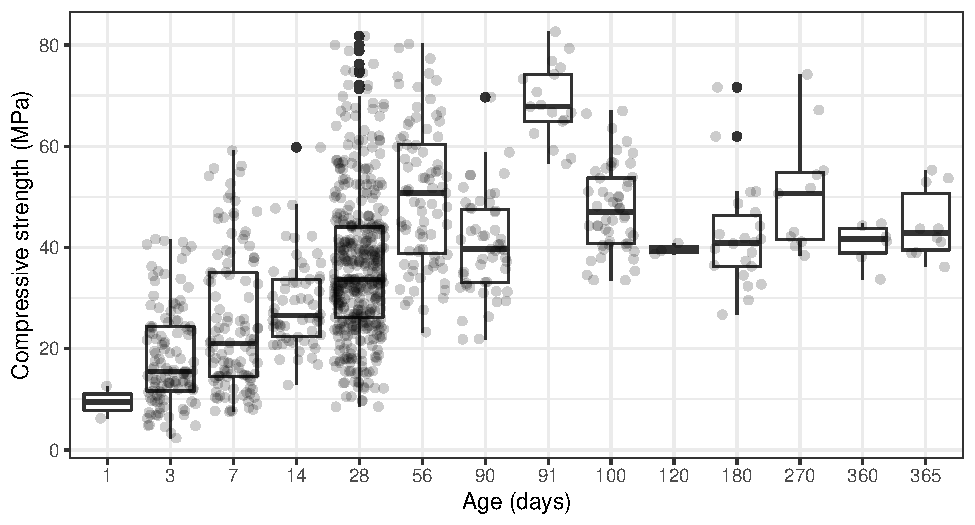
\includegraphics{paper_EN_files/figure-latex/boxplot-1} 

}

\caption{Boxplot - Compressive strength (MPa) vs age (days)}\label{fig:boxplot}
\end{figure}

It was observed that the ages of 90, 91 and 100 days probably represent
extremes to each other in the ingredient configurations, since they are
relatively close ages but with very different values, especially for 90
and 91.

~

This hypothesis was verified using the principal component analysis
method, applied to samples of these 3 ages (\ref{show-pca-90-91-100}).
The figure \ref{fig:pca-90-91-100} shows how the samples relate to each
other (which are similar or different) and revealed how each variable
contributes to the analysis. The first two dimensions represent 37\% and
24\% \$ respectively of the variance.

~

\begin{figure}

{\centering 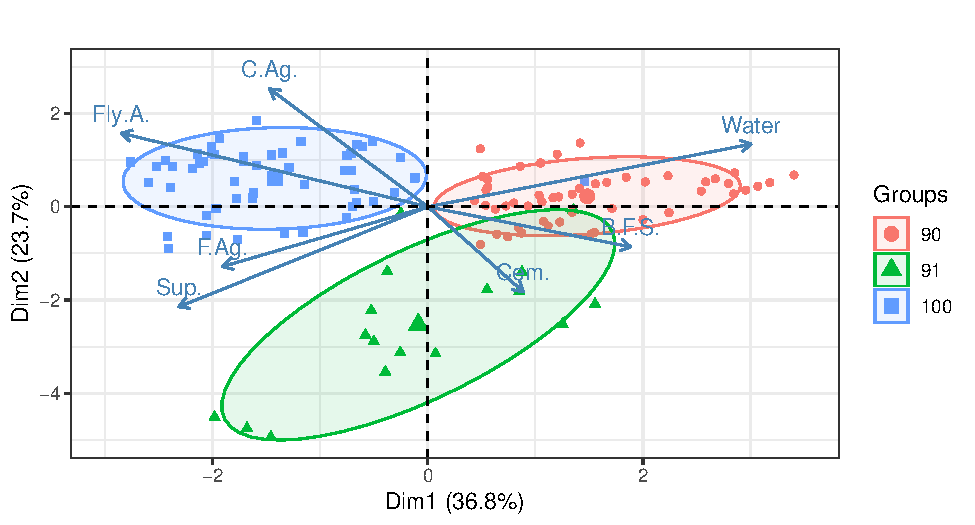
\includegraphics{paper_EN_files/figure-latex/pca-90-91-100-1} 

}

\caption{Principal component analysis - 90, 91 e 100 days}\label{fig:pca-90-91-100}
\end{figure}

Another important point considered, of the concrete nature itself, is
the fact that the growth rate of its compressive strength decreases with
time, reaching a certain stability value. The figure
\ref{fig:mpa-on-time} shows the compressive strength over the days for
samples with more than 5 data, that is, data available for at least 6
different ages (\ref{show-mpa-on-time}).

~

\begin{figure}

{\centering 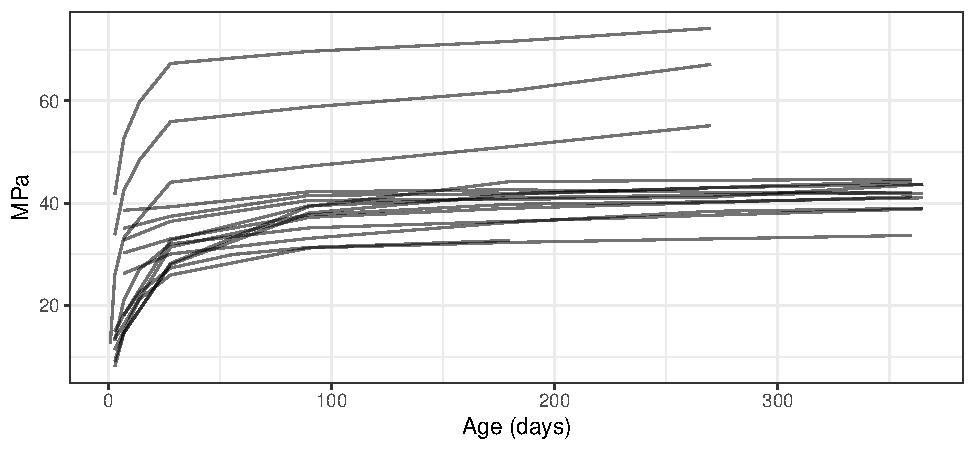
\includegraphics{paper_EN_files/figure-latex/mpa-on-time-1} 

}

\caption{Compressive strength through time}\label{fig:mpa-on-time}
\end{figure}

For the reasons presented in the figures \ref{fig:boxplot},
\ref{fig:pca-90-91-100} and \ref{fig:mpa-on-time}, it was considered
that the ages of 90, 91 and 100 days can be grouped to improve reading
and decrease sample noise. They were converted to the same value, the
age of 100 days was chosen (\ref{show-join-90-91-100}). As shown in the
figure \ref{fig:mpa-on-time}, the resistance only increases, after 100
days the resistance to compression will be greater than or equal to the
value of 90 or 91 days.

~

Another topic analyzed in the selection of ages was the observed
frequency of each age value after this transformation from 90, 91 in 100
days, shown in the figure \ref{fig:freq-ages}. Some values of days have
very low concentrations of samples, at the risk of damaging more than
helping to create the models, so they were removed
(\ref{show-remove-ages-lower-50}). The criterion adopted was to maintain
only ages with a frequency greater than 50, only the values of 3, 7, 14,
28, 56 and 100 days.

~

\begin{figure}

{\centering 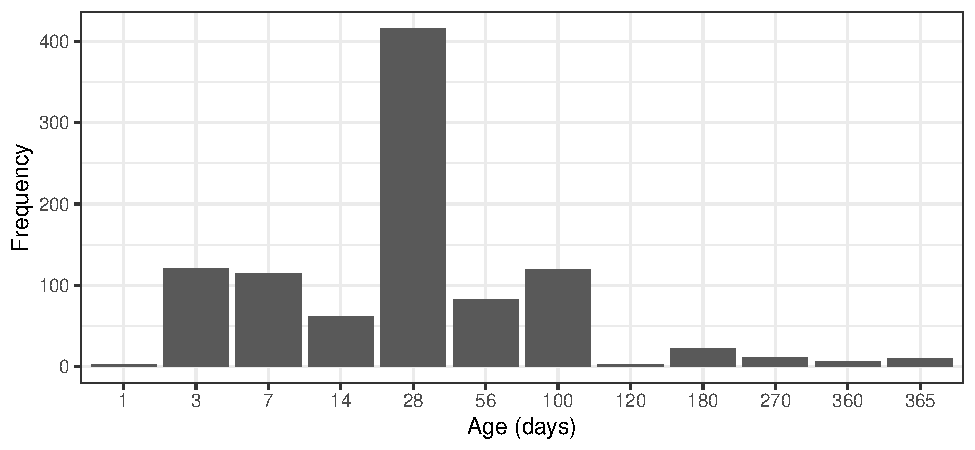
\includegraphics{paper_EN_files/figure-latex/freq-ages-1} 

}

\caption{Ages frequency}\label{fig:freq-ages}
\end{figure}

\hypertarget{data-reorganization}{%
\subsubsection{Data reorganization}\label{data-reorganization}}

The samples were grouped to maintain only one sample from each set of
configuration of the proportions of the ingredients, adding new
variables/columns for resistance at each age
(\ref{show-reorganizing-dat}). The result in the first samples after
this processing is shown in the table \ref{tab:new-features}.

~

\begin{table}[H]

\caption{\label{tab:new-features}First 6 samples after reorganization}
\centering
\resizebox{\linewidth}{!}{
\begin{tabular}[t]{cccccccccccccc}
\toprule
\multicolumn{1}{c}{ID} & \multicolumn{1}{c}{Cement} & \multicolumn{1}{c}{B.F.S} & \multicolumn{1}{c}{Fly ash} & \multicolumn{1}{c}{Water} & \multicolumn{1}{c}{Superp.} & \multicolumn{1}{c}{Coarse Ag.} & \multicolumn{1}{c}{Fine Ag.} & \multicolumn{1}{c}{3 days} & \multicolumn{1}{c}{7 days} & \multicolumn{1}{c}{14 days} & \multicolumn{1}{c}{28 days} & \multicolumn{1}{c}{56 days} & \multicolumn{1}{c}{100 days} \\
 & $kg/m^3$ & $kg/m^3$ & $kg/m^3$ & $kg/m^3$ & $kg/m^3$ & $kg/m^3$ & $kg/m^3$ & $MPa$ & $MPa$ & $MPa$ & $MPa$ & $MPa$ & $MPa$\\
\midrule
1 & 540.0 & 0.0 & 0 & 162 & 2.5 & 1040.0 & 676.0 &  &  &  & 79.99 &  & \\
\addlinespace
2 & 540.0 & 0.0 & 0 & 162 & 2.5 & 1055.0 & 676.0 &  &  &  & 61.89 &  & \\
\addlinespace
3 & 332.5 & 142.5 & 0 & 228 & 0.0 & 932.0 & 594.0 &  & 30.28 &  & 33.02 &  & 37.72\\
\addlinespace
5 & 198.6 & 132.4 & 0 & 192 & 0.0 & 978.4 & 825.5 & 9.13 & 14.64 &  & 28.02 &  & 38.07\\
\addlinespace
6 & 266.0 & 114.0 & 0 & 228 & 0.0 & 932.0 & 670.0 &  &  &  & 45.85 &  & 47.03\\
\addlinespace
7 & 380.0 & 95.0 & 0 & 228 & 0.0 & 932.0 & 594.0 &  & 32.82 &  & 36.45 &  & 40.56\\
\bottomrule
\end{tabular}}
\end{table}

The number of samples and distinct samples after all this manipulation
remained the same, a total of 416 (\ref{show-total-samples-2}).

\hypertarget{adding-new-variables}{%
\subsubsection{Adding new variables}\label{adding-new-variables}}

To finish the data preparation, new columns were added to the dataset
(\ref{show-new-features-2}). Starting with the concrete class, for
example if the compressive strength is between 25 and 30, it receives
the class \emph{C25}. The inclusion of the class was important because
the compressive strength in \emph{MPa} is a continuous variable, which
will be used in the regression models, but the class as a discrete
variable can provide another visualization of the data. The approximate
mix of concrete was also added, which represents the proportions of
aggregates (fine and coarse) for cement. Other proportions between the
main ingredients were also added. The new variables are presented in the
table \ref{tab:new-features-table}.

\begin{table}[H]

\caption{\label{tab:new-features-table}New features}
\centering
\resizebox{\linewidth}{!}{
\begin{tabular}[t]{c>{\centering\arraybackslash}p{1.5cm}>{\centering\arraybackslash}p{2cm}>{\centering\arraybackslash}p{1.7cm}>{\centering\arraybackslash}p{1.7cm}>{\centering\arraybackslash}p{1.7cm}>{\centering\arraybackslash}p{1.7cm}>{\centering\arraybackslash}p{1.7cm}>{\centering\arraybackslash}p{1.7cm}}
\toprule
ID & Class & Approximated Mix & Water / Cement & Fine Ag. / Cement & Coarse Ag. / Cement & Fine Ag. / Coarse Ag. & Water / Coarse Ag. & Water / Fine Ag.\\
\midrule
1 & C75 & 1:1:2 & 0.3000 & 1.2519 & 1.9259 & 0.6500 & 0.1558 & 0.2396\\
\addlinespace
2 & C60 & 1:1:2 & 0.3000 & 1.2519 & 1.9537 & 0.6408 & 0.1536 & 0.2396\\
\addlinespace
3 & C30 & 1:2:3 & 0.6857 & 1.7865 & 2.8030 & 0.6373 & 0.2446 & 0.3838\\
\addlinespace
5 & C25 & 1:4:5 & 0.9668 & 4.1566 & 4.9265 & 0.8437 & 0.1962 & 0.2326\\
\addlinespace
6 & C45 & 1:3:4 & 0.8571 & 2.5188 & 3.5038 & 0.7189 & 0.2446 & 0.3403\\
\addlinespace
7 & C35 & 1:2:2 & 0.6000 & 1.5632 & 2.4526 & 0.6373 & 0.2446 & 0.3838\\
\bottomrule
\end{tabular}}
\end{table}

\hypertarget{data-visualization}{%
\subsection{Data visualization}\label{data-visualization}}

In order to assess the need for further manipulation before building the
models, in this step the 416 samples already processed were visualized
and analyzed.

\hypertarget{descriptive-statistics}{%
\subsubsection{Descriptive statistics}\label{descriptive-statistics}}

The table \ref{tab:stat-summ} presents the statistical data of the
continuous variables (\ref {show-stat-summ}). The \emph{Null} line
represents the number of zeroed values for the ingredients, and the
\emph{NA} line represents the number of missing data. As the samples
were filtered to maintain only sets of samples with known values of
compressive strength at 28 days, the number of \emph{NAs} is zero for
that age. The figure \ref{fig:stat-summ-categorical} presents the
statistical data of the discrete variables
(\ref{show-stat-summ-categorical}).

~

\begin{table}[H]

\caption{\label{tab:stat-summ}Descriptive statistics - continuous variables}
\centering
\resizebox{\linewidth}{!}{
\begin{tabular}[t]{>{\raggedright\arraybackslash}p{1.5cm}cccccccc>{\centering\arraybackslash}p{1.5cm}>{\centering\arraybackslash}p{1.5cm}>{\centering\arraybackslash}p{1.5cm}>{\centering\arraybackslash}p{1.5cm}>{\centering\arraybackslash}p{1.5cm}>{\centering\arraybackslash}p{1.5cm}}
\toprule
  & Samples & Null & NA & Min & Max & Range & Sum & Median & Mean & SE mean & CI mean & Variance & Std.Dev. & Coef.Var\\
\midrule
Cement & 416 & 0 & 0 & 102.00 & 540.00 & 438.00 & 109373.10 & 257.70 & 262.92 & 5.10 & 10.02 & 10817.50 & 104.01 & 0.40\\
\addlinespace
B.F.S. & 416 & 174 & 0 & 0.00 & 359.40 & 359.40 & 35824.60 & 94.25 & 86.12 & 4.32 & 8.49 & 7755.00 & 88.06 & 1.02\\
\addlinespace
Fly ash & 416 & 202 & 0 & 0.00 & 200.10 & 200.10 & 26389.00 & 71.25 & 63.44 & 3.26 & 6.40 & 4407.81 & 66.39 & 1.05\\
\addlinespace
Water & 416 & 0 & 0 & 121.80 & 247.00 & 125.20 & 76335.60 & 185.00 & 183.50 & 0.94 & 1.86 & 370.73 & 19.25 & 0.10\\
\addlinespace
Superplast. & 416 & 107 & 0 & 0.00 & 32.20 & 32.20 & 2871.30 & 7.60 & 6.90 & 0.26 & 0.52 & 28.85 & 5.37 & 0.78\\
\addlinespace
Coarse agg. & 416 & 0 & 0 & 801.00 & 1145.00 & 344.00 & 397799.90 & 953.35 & 956.25 & 4.12 & 8.10 & 7063.06 & 84.04 & 0.09\\
\addlinespace
Fine agg. & 416 & 0 & 0 & 594.00 & 992.60 & 398.60 & 317809.80 & 769.65 & 763.97 & 3.59 & 7.06 & 5371.89 & 73.29 & 0.10\\
\addlinespace
3 days & 121 & 0 & 295 & 2.33 & 41.64 & 39.31 & 2210.82 & 15.52 & 18.27 & 0.87 & 1.72 & 91.64 & 9.57 & 0.52\\
\addlinespace
7 days & 114 & 0 & 302 & 7.51 & 59.09 & 51.58 & 2845.52 & 21.06 & 24.96 & 1.29 & 2.55 & 188.81 & 13.74 & 0.55\\
\addlinespace
14 days & 62 & 0 & 354 & 12.84 & 59.76 & 46.92 & 1782.56 & 26.54 & 28.75 & 1.10 & 2.19 & 74.62 & 8.64 & 0.30\\
\addlinespace
28 days & 416 & 0 & 0 & 8.54 & 81.75 & 73.21 & 15101.13 & 33.72 & 36.30 & 0.70 & 1.38 & 206.30 & 14.36 & 0.40\\
\addlinespace
56 days & 83 & 0 & 333 & 23.25 & 80.20 & 56.95 & 4178.77 & 50.77 & 50.35 & 1.52 & 3.02 & 190.82 & 13.81 & 0.27\\
\addlinespace
100 days & 120 & 0 & 296 & 21.86 & 82.60 & 60.74 & 5701.90 & 45.61 & 47.52 & 1.17 & 2.31 & 163.40 & 12.78 & 0.27\\
\addlinespace
Water / Cement & 416 & 0 & 0 & 0.27 & 1.88 & 1.62 & 340.60 & 0.73 & 0.82 & 0.02 & 0.03 & 0.11 & 0.34 & 0.41\\
\addlinespace
Fine agg. / Cement & 416 & 0 & 0 & 1.14 & 9.24 & 8.10 & 1415.82 & 2.94 & 3.40 & 0.07 & 0.14 & 1.96 & 1.40 & 0.41\\
\addlinespace
Coarse agg. / Cement & 416 & 0 & 0 & 1.55 & 8.70 & 7.14 & 1761.06 & 3.67 & 4.23 & 0.08 & 0.16 & 2.70 & 1.64 & 0.39\\
\addlinespace
Fine agg. / Coarse agg. & 416 & 0 & 0 & 0.53 & 1.16 & 0.63 & 335.42 & 0.80 & 0.81 & 0.01 & 0.01 & 0.01 & 0.11 & 0.14\\
\addlinespace
Water / Coarse agg. & 416 & 0 & 0 & 0.12 & 0.29 & 0.17 & 80.66 & 0.19 & 0.19 & 0.00 & 0.00 & 0.00 & 0.03 & 0.16\\
\addlinespace
Water / Fine agg. & 416 & 0 & 0 & 0.13 & 0.38 & 0.26 & 101.26 & 0.24 & 0.24 & 0.00 & 0.00 & 0.00 & 0.04 & 0.17\\
\bottomrule
\end{tabular}}
\end{table}

\begin{figure}

{\centering 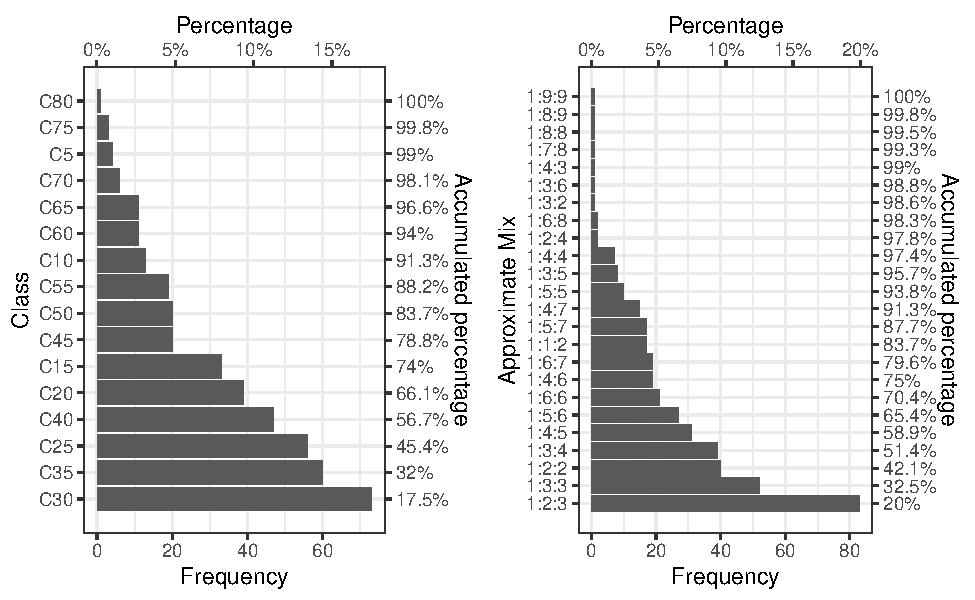
\includegraphics{paper_EN_files/figure-latex/stat-summ-categorical-1} 

}

\caption{Descriptive statistics - categorical variables}\label{fig:stat-summ-categorical}
\end{figure}

\hypertarget{correlation-between-ingredients-and-compressive-strength}{%
\subsubsection{Correlation between ingredients and compressive
strength}\label{correlation-between-ingredients-and-compressive-strength}}

The figure \ref{fig:correlation} shows the correlation of variables for
each set of ages (\ref{show-correlation}). The figure
\ref{fig:correlation-mpa} presents the same data, but instead of
correlating them all, it only correlates with the compressive strength,
showing the values in more detail (\ref{show-correlation-mpa}).

~

\begin{figure}

{\centering 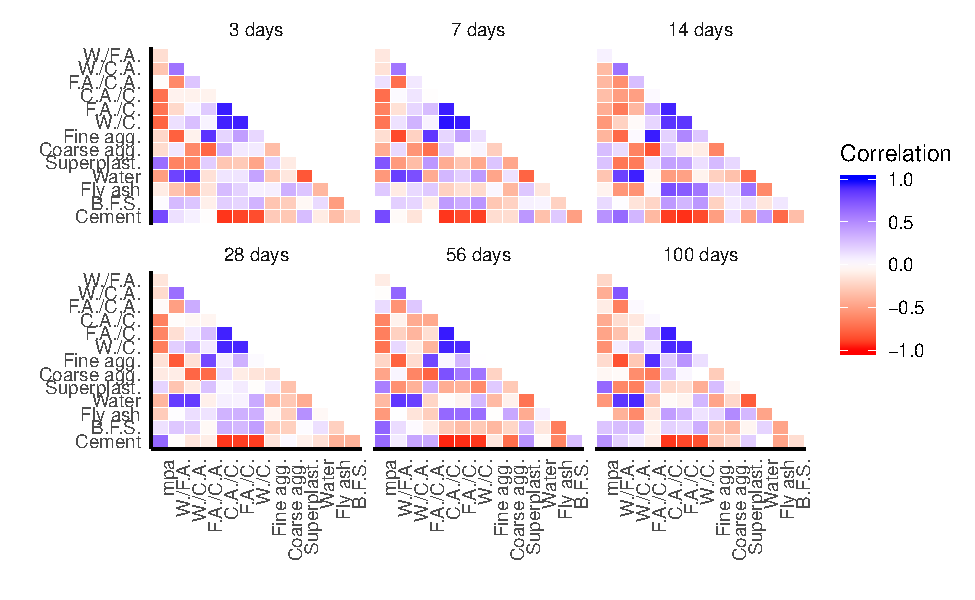
\includegraphics{paper_EN_files/figure-latex/correlation-1} 

}

\caption{Correlations at each age}\label{fig:correlation}
\end{figure}

\begin{figure}

{\centering 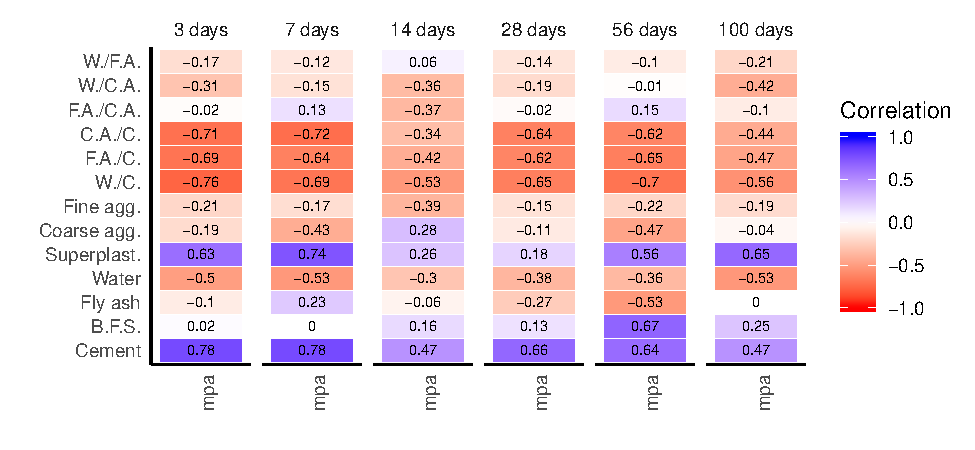
\includegraphics{paper_EN_files/figure-latex/correlation-mpa-1} 

}

\caption{Correlation of variables with compressive strength over time}\label{fig:correlation-mpa}
\end{figure}

The interpretation of the figure \ref{fig:correlation-mpa} suggests that
the strength of the concrete is positively related mainly to the cement
and superplasticizer ingredients and negatively to the water and fine
aggregate. The smaller the amount of cement for aggregates and water,
the more negatively they are correlated with compressive strength.

~

\begin{figure}

{\centering 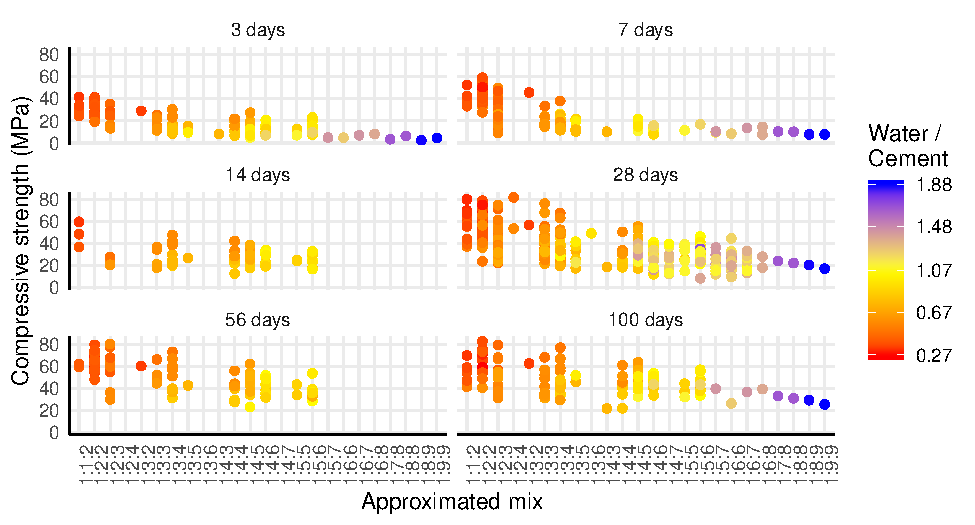
\includegraphics{paper_EN_files/figure-latex/mix-app-mpa-1} 

}

\caption{Relationship between approximated mix, water, MPa and age}\label{fig:mix-app-mpa}
\end{figure}

\begin{figure}

{\centering 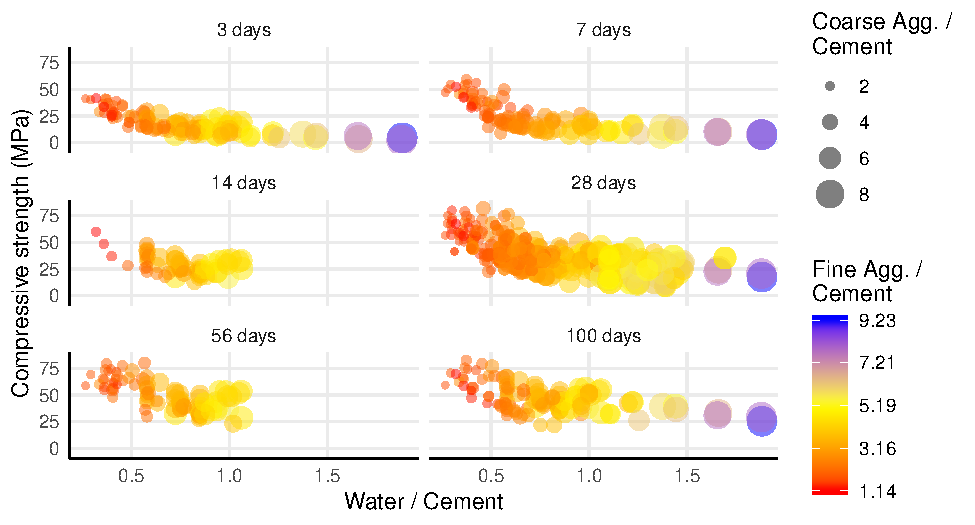
\includegraphics{paper_EN_files/figure-latex/mix-mpa-1} 

}

\caption{Relationship between concrete main features}\label{fig:mix-mpa}
\end{figure}

The figures \ref{fig:mix-app-mpa} and \ref{fig:mix-mpa} show the
relationship between the main ingredients (known as mix) in relation to
the compressive strength (\ref{show-mix-app-mpa} and
\ref{show-mix-mpa}). The interpretation of these figures shows that the
greater the amount of cement in relation to the other ingredients, the
greater the resistance to compression.

\hypertarget{variables-distribution}{%
\subsubsection{Variables distribution}\label{variables-distribution}}

The figure\ref{fig:vars-distribution} shows the distribution of
variables in the samples (\ref{show-vars-distribution}). It was
calculated using data only at 28 days.

~

\begin{figure}

{\centering 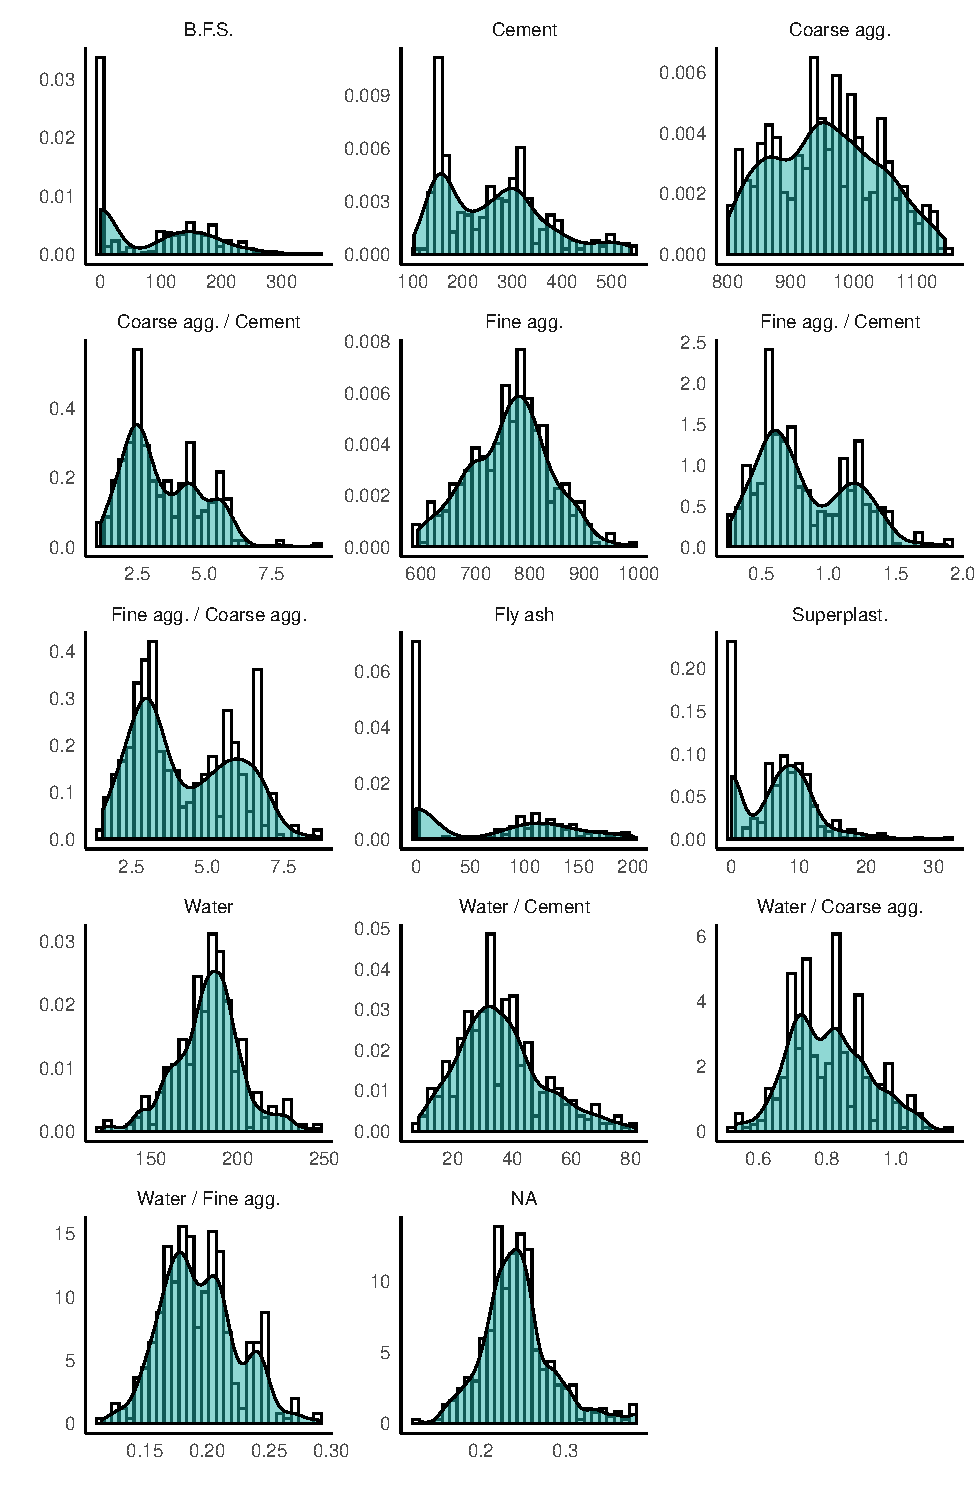
\includegraphics{paper_EN_files/figure-latex/vars-distribution-1} 

}

\caption{Variables distribution}\label{fig:vars-distribution}
\end{figure}

The figure \ref{fig:vars-distribution-time} shows the distribution of
ingredients and compressive strength for each set of ages
(\ref{show-vars-distribution-time}), in case of the 28 days it presents
the same information as the figure \ref{fig:vars-distribution}. It shows
that the resistance to compression gradually increases over time, as
expected. Furthermore it is seen that the concentration of the
ingredients can vary a lot when stratified by ages.

\begin{figure}

{\centering 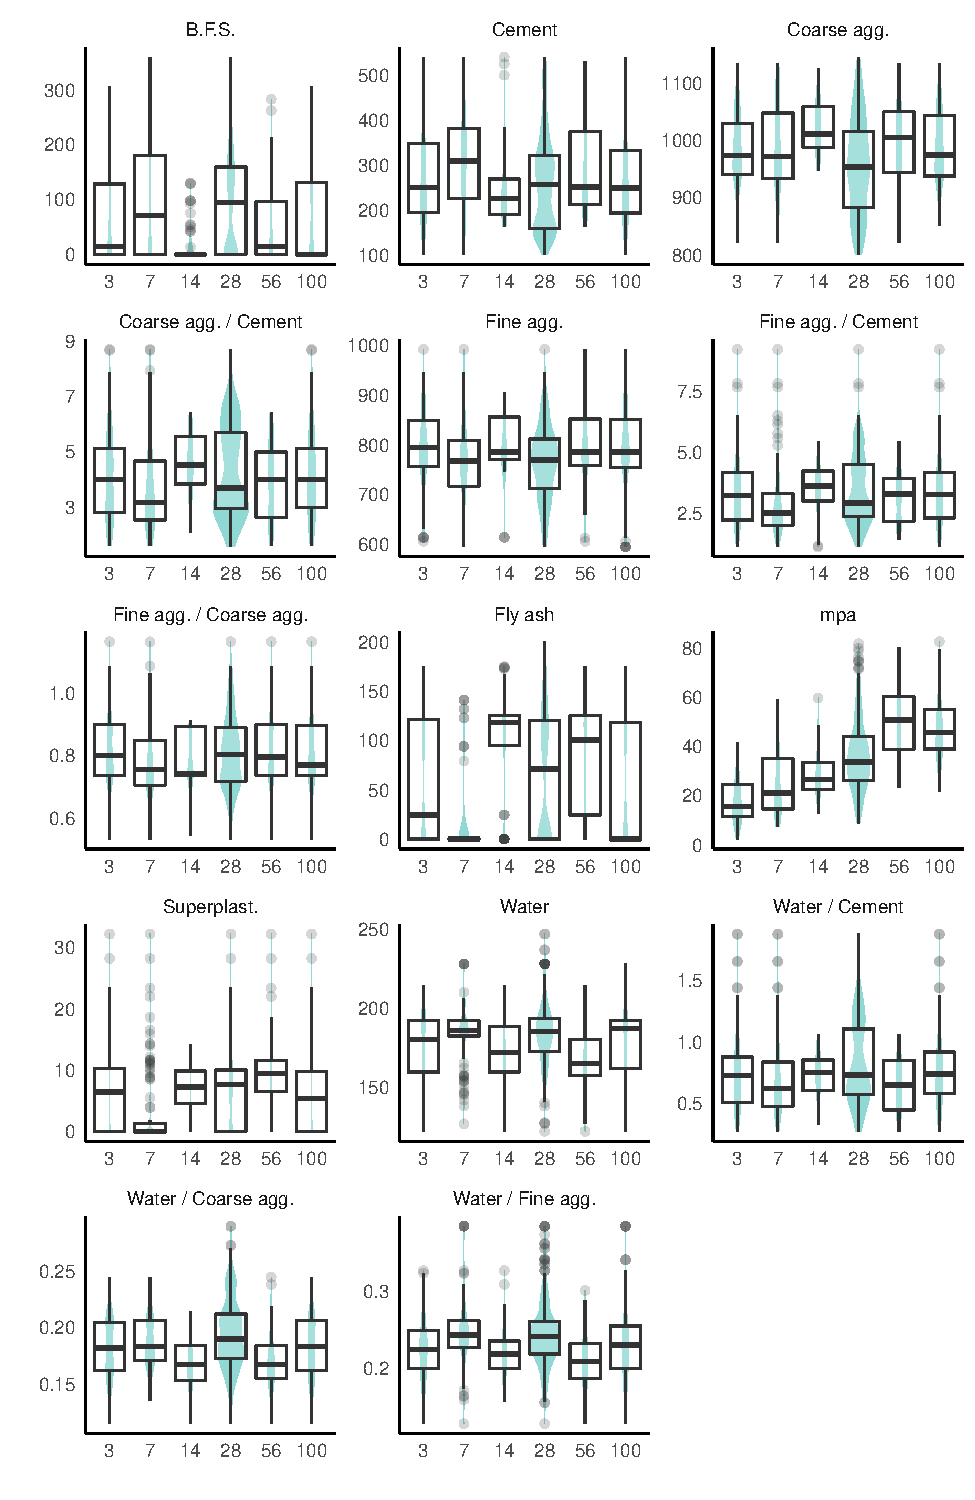
\includegraphics{paper_EN_files/figure-latex/vars-distribution-time-1} 

}

\caption{Variables distribution grouped by age}\label{fig:vars-distribution-time}
\end{figure}

\hypertarget{principal-component-analysis}{%
\subsubsection{Principal component
analysis}\label{principal-component-analysis}}

In the figure \ref{fig:pca}, using an alternative classification, the
principal component analysis was performed on the ingredients
(\ref{show-pca}). The classification separates concrete into 4 different
compressive strength groups, low up to \emph{20 MPa}, normal up to
\emph{40 MPa}, medium up to \emph{70 MPa} and high above that. It is
possible to notice that the groups overlap, but there is a
differentiation between the high and low group.

\begin{figure}

{\centering 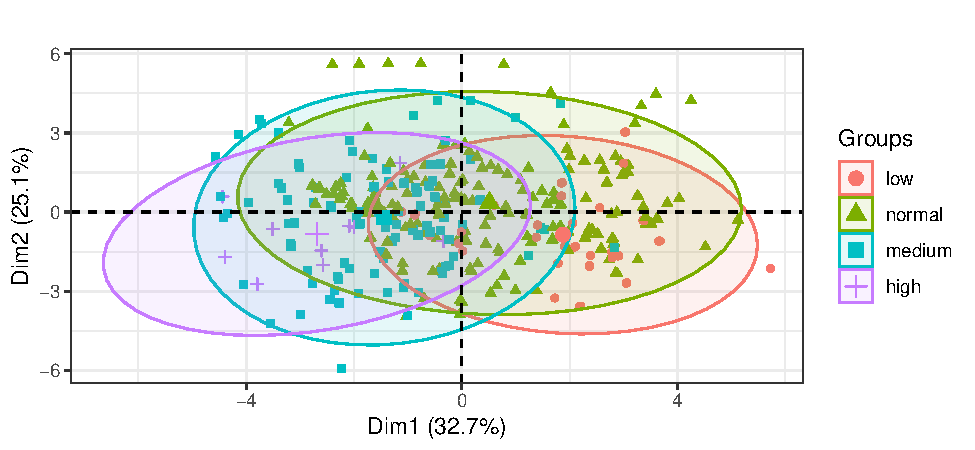
\includegraphics{paper_EN_files/figure-latex/pca-1} 

}

\caption{Principal component analysis on ingredients}\label{fig:pca}
\end{figure}

\hypertarget{machine-learning-models}{%
\subsection{Machine learning models}\label{machine-learning-models}}

The development of machine learning models was carried out with the
\emph{caret} package (Kuhn 2020) and based on Irizarry (2019) and Kuhn
(2008).

\hypertarget{pre-processing-and-data-separation}{%
\subsubsection{Pre-processing and data
separation}\label{pre-processing-and-data-separation}}

As the approximate mix is a categorical variable, it was converted into
dummy variables (\ref{show-dummy-var}), going from 22 columns (id,
class, compressive strength and 19 more \emph{features}) to 45 columns,
an addition of 23 variables, one for each approximate mix.

~

The samples were separated based on age. One dataset was created for
each age value, totaling 6 different sets (\ref{show-preparation}). For
illustrative purposes, the first 18 of 45 columns of the first 6 samples
from the 28-day set are shown in the table
\ref{tab:table-preparated-samples}.

~

\begin{table}[H]

\caption{\label{tab:table-preparated-samples}First 18 columns of the 6 first samples of 28 days}
\centering
\resizebox{\linewidth}{!}{
\begin{tabular}[t]{cccccccccccccccccc}
\toprule
\multicolumn{1}{c}{ID} & \multicolumn{1}{c}{Cement} & \multicolumn{1}{c}{B.F.S.} & \multicolumn{1}{c}{Fly ash} & \multicolumn{1}{c}{water} & \multicolumn{1}{c}{Superp.} & \multicolumn{1}{c}{Coarse Agg.} & \multicolumn{1}{c}{Fine Agg.} & \multicolumn{1}{c}{MPa} & \multicolumn{1}{c}{Class} & \multicolumn{1}{c}{Wat./} & \multicolumn{1}{c}{F.Agg./} & \multicolumn{1}{c}{C.Agg./} & \multicolumn{1}{c}{F.Agg./} & \multicolumn{1}{c}{Wat./} & \multicolumn{1}{c}{Wat./} & \multicolumn{2}{c}{App Mix} \\
 & $kg/m^3$ & $kg/m^3$ & $kg/m^3$ & $kg/m^3$ & $kg/m^3$ & $kg/m^3$ & $kg/m^3$ & $MPa$ &  & Ci. & Ce. & Ce. & C.Agg. & C.Agg. & F.Agg. & 1:1:2 & 1:2:2\\
\midrule
1 & 540.0 & 0.0 & 0 & 162 & 2.5 & 1040.0 & 676.0 & 79.99 & C75 & 0.30 & 1.25 & 1.93 & 0.65 & 0.16 & 0.24 & 1 & 0\\
\addlinespace
2 & 540.0 & 0.0 & 0 & 162 & 2.5 & 1055.0 & 676.0 & 61.89 & C60 & 0.30 & 1.25 & 1.95 & 0.64 & 0.15 & 0.24 & 1 & 0\\
\addlinespace
3 & 332.5 & 142.5 & 0 & 228 & 0.0 & 932.0 & 594.0 & 33.02 & C30 & 0.69 & 1.79 & 2.80 & 0.64 & 0.24 & 0.38 & 0 & 0\\
\addlinespace
5 & 198.6 & 132.4 & 0 & 192 & 0.0 & 978.4 & 825.5 & 28.02 & C25 & 0.97 & 4.16 & 4.93 & 0.84 & 0.20 & 0.23 & 0 & 0\\
\addlinespace
6 & 266.0 & 114.0 & 0 & 228 & 0.0 & 932.0 & 670.0 & 45.85 & C45 & 0.86 & 2.52 & 3.50 & 0.72 & 0.24 & 0.34 & 0 & 0\\
\addlinespace
7 & 380.0 & 95.0 & 0 & 228 & 0.0 & 932.0 & 594.0 & 36.45 & C35 & 0.60 & 1.56 & 2.45 & 0.64 & 0.24 & 0.38 & 0 & 1\\
\bottomrule
\end{tabular}}
\end{table}

For each of the 6 sets, the existence or not of variables with variance
close to zero and their subsequent removal was verified
(\ref{show-nzv}). Many of the 23 variables added referring to the
approximate concrete mix were removed due to this fact. In addition to
them, in the case of the 7-day set, the fly ash variable was also
removed. Then it was verified that there are no variables with high
correlation, above 0.999, in any of the 6 data sets (\ref{show-cors}).
After these steps, the sample sets presented 24, 21, 23, 23, 24 and 25
columns respectively for ages in increasing sequence.

~

The stage of centralization and normalization of the variables was
carried out later, together with the application of the models, as it is
simpler to do this with the \emph{caret} package. If performed at this
time, it would be necessary to manually undo these transformations in
the predictions. The \emph{caret} allows you to transform before
training the models and already transforms the results back.

~

Each data set was separated into test and training sets, \emph{20\%} and
\emph{80\%} respectively (\ref{show-split}). The figure
\ref{fig:dist-split} shows the distribution of data between the sets in
relation to the compressive strength for each model
(\ref{show-dist-split}).

\begin{figure}

{\centering 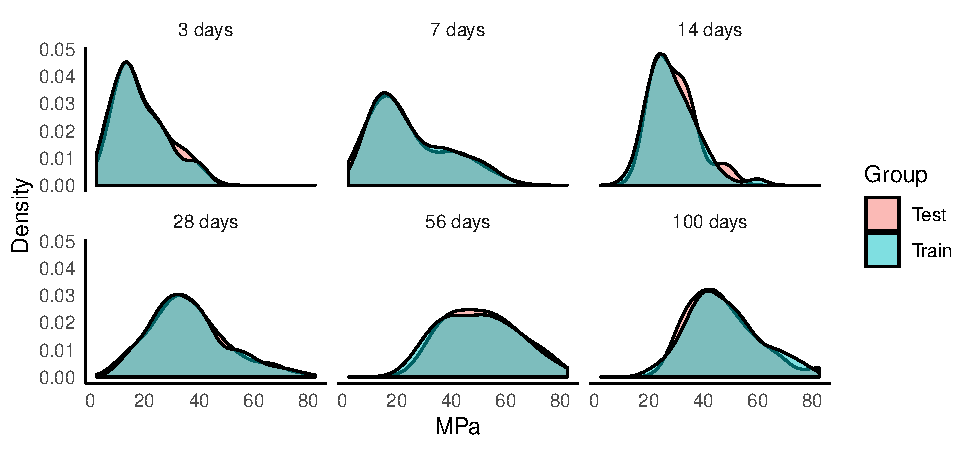
\includegraphics{paper_EN_files/figure-latex/dist-split-1} 

}

\caption{Distribution of test and train data}\label{fig:dist-split}
\end{figure}

\hypertarget{performance-measures}{%
\subsubsection{Performance measures}\label{performance-measures}}

The performance evaluation of the models was performed by the Root Mean
Square Error (\emph{RMSE}). The \emph{RMSE} is the measure used in all
the works mentioned in the introduction and will allow the comparison of
the models in the discussion.

\hypertarget{naive-models}{%
\subsubsection{Naive models}\label{naive-models}}

Before creating the real models, for comparison purposes, naive models
were created. They simply predict that the compressive strength of the
test set is the average compressive strength of the training set
(\ref{show-naive-model-reg}). In other words, naive models are simply
the best guess possible. The results can be checked in the table
\ref{tab:table-naive-model-reg}.

\begin{table}[H]

\caption{\label{tab:table-naive-model-reg}Naive models}
\centering
\begin{tabular}[t]{cccc}
\toprule
Age & Mean $MPa$ (train) & RMSE (train) & RMSE (test)\\
\midrule
3 & 18.08887 & 9.591344 & 9.303229\\
\addlinespace
7 & 25.12383 & 13.731569 & 13.443646\\
\addlinespace
14 & 28.63980 & 8.786823 & 7.593319\\
\addlinespace
28 & 36.33605 & 14.361021 & 14.283824\\
\addlinespace
56 & 50.06555 & 13.968077 & 12.702112\\
\addlinespace
100 & 47.57000 & 12.758042 & 12.614652\\
\bottomrule
\end{tabular}
\end{table}

\hypertarget{choice-of-algorithms}{%
\subsubsection{Choice of algorithms}\label{choice-of-algorithms}}

The \emph{caret} (Kuhn 2020) package exposes more than 200 different
algorithms for building \emph{machine learning} models. The package
documentation presents an initial code (``Models Clustered by Tag
Similarity'' 2020) as a suggestion to select a portfolio of the most
distinct algorithms possible in relation to some pre-selected algorithm,
but for agility and due to technical limitations, it was chosen to use
an algorithm with the highest probability to achieve the best possible
result. According to Fernandez-Delgado et al. (2014), who compared 179
algorithms in 121 different databases, the algorithm most likely to
achieve the best possible results is the \emph{Parallel Random Forest}
(called \emph{prRF } in \emph{caret}).

\hypertarget{regression-models}{%
\subsubsection{Regression models}\label{regression-models}}

As new variables were added throughout the processing (the relationships
between the ingredients and a few more \emph{dummy vars} for each age
set), 5 possibilities for configuring the \emph{features} for the models
were studied:

~

\begin{enumerate}
\def\labelenumi{\arabic{enumi}.}
\tightlist
\item
  All \emph{features};
\item
  All \emph{features} without the \emph{dummy vars};
\item
  Only the original \emph{features};
\item
  Only new \emph{features};
\item
  Only new \emph{features}, without \emph{dummy vars};
\end{enumerate}

~

Building a model for each of these configurations using the set at 28
days (\ref{show-test-models-reg}), showed that the best option is
configuration 2, the \emph{dummy vars} were completely discarded, but
the other new variables were kept. For illustrative purposes, the
\ref{tab:table-done-samples-28} table shows the first 6 samples from the
28-day model training set. The samples of the other models, of the test
and training sets are similar, the only difference being in the 7-day
model, which excludes fly ash due to the variance close to zero,
performed previously.

\begin{table}[H]

\caption{\label{tab:table-done-samples-28}First 6 samples of train data of the 28 days model}
\centering
\resizebox{\linewidth}{!}{
\begin{tabular}[t]{cccccccccccccc}
\toprule
\multicolumn{13}{c}{Features} & \multicolumn{1}{c}{Outcome} \\
\cmidrule(l{3pt}r{3pt}){1-13} \cmidrule(l{3pt}r{3pt}){14-14}
\multicolumn{1}{c}{Cement} & \multicolumn{1}{c}{B.F.S.} & \multicolumn{1}{c}{Fly ash} & \multicolumn{1}{c}{water} & \multicolumn{1}{c}{Superp.} & \multicolumn{1}{c}{Coarse Agg.} & \multicolumn{1}{c}{Fine Agg.} & \multicolumn{1}{c}{Wat./} & \multicolumn{1}{c}{F.Agg./} & \multicolumn{1}{c}{C.Agg./} & \multicolumn{1}{c}{F.Agg./} & \multicolumn{1}{c}{Wat./} & \multicolumn{1}{c}{Wat./} & \multicolumn{1}{c}{y} \\
$kg/m^3$ & $kg/m^3$ & $kg/m^3$ & $kg/m^3$ & $kg/m^3$ & $kg/m^3$ & $kg/m^3$ & Ce. & Ce. & Ce. & C.Agg. & C.Agg. & F.Agg. & MPa\\
\midrule
540.0 & 0.0 & 0 & 162 & 2.5 & 1040.0 & 676.0 & 0.30 & 1.25 & 1.93 & 0.65 & 0.16 & 0.24 & 79.99\\
\addlinespace
540.0 & 0.0 & 0 & 162 & 2.5 & 1055.0 & 676.0 & 0.30 & 1.25 & 1.95 & 0.64 & 0.15 & 0.24 & 61.89\\
\addlinespace
266.0 & 114.0 & 0 & 228 & 0.0 & 932.0 & 670.0 & 0.86 & 2.52 & 3.50 & 0.72 & 0.24 & 0.34 & 45.85\\
\addlinespace
380.0 & 95.0 & 0 & 228 & 0.0 & 932.0 & 594.0 & 0.60 & 1.56 & 2.45 & 0.64 & 0.24 & 0.38 & 36.45\\
\addlinespace
475.0 & 0.0 & 0 & 228 & 0.0 & 932.0 & 594.0 & 0.48 & 1.25 & 1.96 & 0.64 & 0.24 & 0.38 & 39.29\\
\addlinespace
198.6 & 132.4 & 0 & 192 & 0.0 & 978.4 & 825.5 & 0.97 & 4.16 & 4.93 & 0.84 & 0.20 & 0.23 & 28.02\\
\bottomrule
\end{tabular}}
\end{table}

For each age set, a model was created using the \emph{Parallel Random
Forest} algorithm, previously defined (\ref{show-reg-models}). For each
of the 6 models, the parameter \emph{mtry} was optimized, and
\emph{repeated cross-validation } was performed, dividing into 10 or 30
parts and repeating 10 times.

\hypertarget{results}{%
\section{Results}\label{results}}

The test \emph{RMSE} for each model in ascending order of age was 3.31,
4.36, 4.62, 4.72, 5.94 and 5.85 respectively. The table
\ref{tab:table-reg-models} presents the details and results of each
model (\ref{show-table-reg-models}). The figure
\ref{fig:results-comparison} compares the actual and predicted values
(\ref{show-results-comparison}), and the following tables show the best
and worst results for each model (\ref{show-table-10}).

\begin{table}[H]

\caption{\label{tab:table-reg-models}Regression models results}
\centering
\begin{tabular}[t]{cccccc}
\toprule
Model & mtry & CV & Repetitions & RMSE (train) & RMSE (test)\\
\midrule
3 days & 6 & 30 & 10 & 3.905196 & 3.310370\\
\addlinespace
7 days & 2 & 10 & 10 & 4.475981 & 4.361987\\
\addlinespace
14 days & 13 & 30 & 10 & 5.136687 & 4.620515\\
\addlinespace
28 days & 11 & 30 & 10 & 5.847334 & 4.716698\\
\addlinespace
56 days & 8 & 30 & 10 & 6.702565 & 5.939163\\
\addlinespace
100 days & 8 & 10 & 10 & 6.381940 & 5.851088\\
\bottomrule
\end{tabular}
\end{table}

\begin{figure}

{\centering 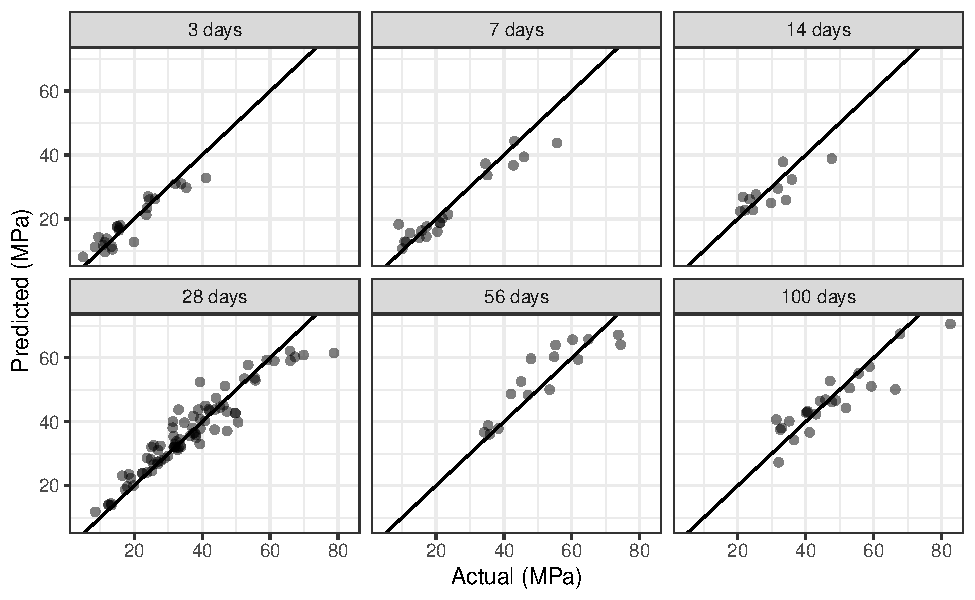
\includegraphics{paper_EN_files/figure-latex/results-comparison-1} 

}

\caption{Actual vs Predicted values in each model}\label{fig:results-comparison}
\end{figure}

\begin{table}[H]

\caption{\label{tab:table-10}Model of 3 days}
\centering
\begin{tabular}[t]{ccc>{\centering\arraybackslash}p{1cm}ccc}
\toprule
\multicolumn{3}{c}{Best 10} & \multicolumn{1}{c}{} & \multicolumn{3}{c}{Worst 10} \\
\cmidrule(l{3pt}r{3pt}){1-3} \cmidrule(l{3pt}r{3pt}){5-7}
Actual & Predicted & Error &  & Actual & Predicted & Error\\
\midrule
26.06 & 26.297746 & 0.2377457 &  & 41.10 & 32.758262 & -8.341738\\
\addlinespace
23.80 & 23.432367 & -0.3676333 &  & 19.93 & 12.732172 & -7.197828\\
\addlinespace
15.52 & 16.436292 & 0.9162920 &  & 35.30 & 29.781989 & -5.518011\\
\addlinespace
10.76 & 11.830651 & 1.0706507 &  & 9.45 & 14.316742 & 4.866742\\
\addlinespace
32.11 & 30.977619 & -1.1323807 &  & 4.90 & 8.154245 & 3.254245\\
\addlinespace
11.36 & 12.660044 & 1.3000440 &  & 13.57 & 10.464572 & -3.105428\\
\addlinespace
15.62 & 17.079698 & 1.4596980 &  & 24.10 & 27.016321 & 2.916321\\
\addlinespace
24.39 & 26.018261 & 1.6282610 &  & 33.80 & 31.045796 & -2.754204\\
\addlinespace
11.41 & 9.688879 & -1.7211213 &  & 8.49 & 11.196910 & 2.706910\\
\addlinespace
11.85 & 13.788864 & 1.9388640 &  & 14.99 & 17.677379 & 2.687379\\
\bottomrule
\end{tabular}
\end{table}

\begin{table}[H]

\caption{\label{tab:table-10}Model of 7 days}
\centering
\begin{tabular}[t]{ccc>{\centering\arraybackslash}p{1cm}ccc}
\toprule
\multicolumn{3}{c}{Best 10} & \multicolumn{1}{c}{} & \multicolumn{3}{c}{Worst 10} \\
\cmidrule(l{3pt}r{3pt}){1-3} \cmidrule(l{3pt}r{3pt}){5-7}
Actual & Predicted & Error &  & Actual & Predicted & Error\\
\midrule
17.24 & 17.61947 & 0.3794733 &  & 55.60 & 43.71082 & -11.889177\\
\addlinespace
15.75 & 16.29318 & 0.5431847 &  & 9.01 & 18.32999 & 9.319987\\
\addlinespace
10.09 & 10.67438 & 0.5843837 &  & 45.90 & 39.45277 & -6.447230\\
\addlinespace
15.07 & 14.10010 & -0.9698955 &  & 42.80 & 36.78526 & -6.014737\\
\addlinespace
43.11 & 44.35190 & 1.2419040 &  & 20.42 & 16.03647 & -4.383533\\
\addlinespace
35.10 & 33.69951 & -1.4004926 &  & 12.37 & 15.58829 & 3.218292\\
\addlinespace
11.17 & 12.71080 & 1.5408013 &  & 17.17 & 14.38220 & -2.787795\\
\addlinespace
21.86 & 20.23260 & -1.6274033 &  & 34.57 & 37.26745 & 2.697450\\
\addlinespace
10.79 & 12.85092 & 2.0609233 &  & 21.16 & 18.79017 & -2.369827\\
\addlinespace
23.52 & 21.42631 & -2.0936880 &  & 21.18 & 18.84231 & -2.337694\\
\bottomrule
\end{tabular}
\end{table}

\begin{table}[H]

\caption{\label{tab:table-10}Model of 14 days}
\centering
\begin{tabular}[t]{ccc>{\centering\arraybackslash}p{1cm}ccc}
\toprule
\multicolumn{3}{c}{Best 10} & \multicolumn{1}{c}{} & \multicolumn{3}{c}{Worst 10} \\
\cmidrule(l{3pt}r{3pt}){1-3} \cmidrule(l{3pt}r{3pt}){5-7}
Actual & Predicted & Error &  & Actual & Predicted & Error\\
\midrule
22.14 & 22.69248 & 0.5524823 &  & 47.71 & 38.87416 & -8.835845\\
\addlinespace
20.77 & 22.36561 & 1.5956093 &  & 34.24 & 25.88502 & -8.354984\\
\addlinespace
24.45 & 22.74412 & -1.7058757 &  & 21.50 & 26.91740 & 5.417403\\
\addlinespace
25.37 & 27.62261 & 2.2526130 &  & 29.75 & 25.02926 & -4.720744\\
\addlinespace
31.81 & 29.53499 & -2.2750130 &  & 33.36 & 37.88168 & 4.521675\\
\addlinespace
23.51 & 26.19615 & 2.6861493 &  & 35.96 & 32.35358 & -3.606417\\
\addlinespace
35.96 & 32.35358 & -3.6064167 &  & 23.51 & 26.19615 & 2.686149\\
\addlinespace
33.36 & 37.88168 & 4.5216750 &  & 31.81 & 29.53499 & -2.275013\\
\addlinespace
29.75 & 25.02926 & -4.7207443 &  & 25.37 & 27.62261 & 2.252613\\
\addlinespace
21.50 & 26.91740 & 5.4174030 &  & 24.45 & 22.74412 & -1.705876\\
\bottomrule
\end{tabular}
\end{table}

\begin{table}[H]

\caption{\label{tab:table-10}Model of 28 days}
\centering
\begin{tabular}[t]{ccc>{\centering\arraybackslash}p{1cm}ccc}
\toprule
\multicolumn{3}{c}{Best 10} & \multicolumn{1}{c}{} & \multicolumn{3}{c}{Worst 10} \\
\cmidrule(l{3pt}r{3pt}){1-3} \cmidrule(l{3pt}r{3pt}){5-7}
Actual & Predicted & Error &  & Actual & Predicted & Error\\
\midrule
27.83 & 27.86776 & 0.0377573 &  & 78.80 & 61.57401 & -17.225986\\
\addlinespace
43.80 & 43.84951 & 0.0495087 &  & 39.38 & 52.47227 & 13.092267\\
\addlinespace
26.92 & 26.82812 & -0.0918800 &  & 33.04 & 43.81819 & 10.778193\\
\addlinespace
31.87 & 32.06794 & 0.1979360 &  & 50.60 & 39.85258 & -10.747415\\
\addlinespace
19.77 & 19.97517 & 0.2051693 &  & 47.40 & 37.11150 & -10.288501\\
\addlinespace
31.88 & 32.13467 & 0.2546680 &  & 69.84 & 60.88636 & -8.953635\\
\addlinespace
59.00 & 59.36857 & 0.3685727 &  & 31.38 & 40.09934 & 8.719345\\
\addlinespace
23.79 & 24.17376 & 0.3837583 &  & 49.77 & 42.71779 & -7.052213\\
\addlinespace
28.99 & 28.55592 & -0.4340790 &  & 49.77 & 42.72394 & -7.046057\\
\addlinespace
32.24 & 31.79166 & -0.4483390 &  & 25.10 & 32.07616 & 6.976158\\
\bottomrule
\end{tabular}
\end{table}

\begin{table}[H]

\caption{\label{tab:table-10}Model of 56 days}
\centering
\begin{tabular}[t]{ccc>{\centering\arraybackslash}p{1cm}ccc}
\toprule
\multicolumn{3}{c}{Best 10} & \multicolumn{1}{c}{} & \multicolumn{3}{c}{Worst 10} \\
\cmidrule(l{3pt}r{3pt}){1-3} \cmidrule(l{3pt}r{3pt}){5-7}
Actual & Predicted & Error &  & Actual & Predicted & Error\\
\midrule
35.85 & 36.06413 & 0.2141317 &  & 47.97 & 59.74774 & 11.777736\\
\addlinespace
38.33 & 37.86955 & -0.4604540 &  & 74.36 & 64.08547 & -10.274529\\
\addlinespace
64.90 & 65.81326 & 0.9132646 &  & 55.20 & 64.00472 & 8.804718\\
\addlinespace
47.13 & 48.41224 & 1.2822413 &  & 45.08 & 52.62057 & 7.540568\\
\addlinespace
61.86 & 59.49031 & -2.3696857 &  & 42.03 & 48.63652 & 6.606522\\
\addlinespace
34.20 & 36.72639 & 2.5263850 &  & 73.70 & 67.19523 & -6.504768\\
\addlinespace
53.46 & 50.04835 & -3.4116453 &  & 54.77 & 60.36449 & 5.594488\\
\addlinespace
35.34 & 38.82656 & 3.4865560 &  & 60.20 & 65.67068 & 5.470680\\
\addlinespace
60.20 & 65.67068 & 5.4706798 &  & 35.34 & 38.82656 & 3.486556\\
\addlinespace
54.77 & 60.36449 & 5.5944884 &  & 53.46 & 50.04835 & -3.411645\\
\bottomrule
\end{tabular}
\end{table}

\begin{table}[H]

\caption{\label{tab:table-10}Model of 100 days}
\centering
\begin{tabular}[t]{ccc>{\centering\arraybackslash}p{1cm}ccc}
\toprule
\multicolumn{3}{c}{Best 10} & \multicolumn{1}{c}{} & \multicolumn{3}{c}{Worst 10} \\
\cmidrule(l{3pt}r{3pt}){1-3} \cmidrule(l{3pt}r{3pt}){5-7}
Actual & Predicted & Error &  & Actual & Predicted & Error\\
\midrule
67.80 & 67.53752 & -0.2624793 &  & 66.42 & 50.11266 & -16.307345\\
\addlinespace
55.64 & 55.13289 & -0.5071103 &  & 82.60 & 70.59383 & -12.006168\\
\addlinespace
43.06 & 42.33515 & -0.7248493 &  & 31.35 & 40.69152 & 9.341519\\
\addlinespace
45.84 & 46.89673 & 1.0567320 &  & 59.30 & 51.07318 & -8.226824\\
\addlinespace
47.74 & 46.24704 & -1.4929567 &  & 51.86 & 44.27586 & -7.584144\\
\addlinespace
58.78 & 57.23738 & -1.5426163 &  & 47.22 & 52.72019 & 5.500191\\
\addlinespace
48.85 & 46.67286 & -2.1771403 &  & 32.92 & 38.02416 & 5.104161\\
\addlinespace
44.21 & 46.50377 & 2.2937710 &  & 32.53 & 37.56541 & 5.035406\\
\addlinespace
36.59 & 34.26929 & -2.3207093 &  & 35.17 & 40.18011 & 5.010112\\
\addlinespace
52.96 & 50.52831 & -2.4316947 &  & 32.07 & 27.31722 & -4.752779\\
\bottomrule
\end{tabular}
\end{table}

\hypertarget{discussion-and-conclusion}{%
\section{Discussion and conclusion}\label{discussion-and-conclusion}}

The models built present satisfactory results and prove that the
compressive strength of concrete can be predicted relatively easily. The
alternative adopted to create a model for each set of age proved to be a
valid method, managing to stratify to obtain specific results for each
set. The studies cited in the introduction using the same dataset have
similar results, as expected. The \ref{tab:works-comparison} table
presents the results of these works (\ref{show-works-comparison}), and
the table \ref{tab:results} presents the values found for easy
comparison (\ref{show-results}).

\begin{table}[H]

\caption{\label{tab:works-comparison}Comparison of other works}
\centering
\begin{tabular}[t]{llll}
\toprule
Author & Year & Algorithm & RMSE\\
\midrule
Pierobon & 2018 & Ensemble com 5 algorítimos & 4.150\\
\addlinespace
Hameed & 2020 & Artificial Neural Networks & 4.736\\
\addlinespace
Raj & 2018 & Gradient Boosting Regressor & 4.957\\
\addlinespace
Modukuru & 2020 & Random Forest Regressor & 5.080\\
\addlinespace
Alshamiri & 2020 & Regularized Extreme Learning Machine & 5.508\\
\addlinespace
Abban & 2016 & Support Vector Machines with Radial Basis Function Kernel & 6.105\\
\bottomrule
\end{tabular}
\end{table}

\begin{table}[H]

\caption{\label{tab:results}Final result}
\centering
\begin{tabular}[t]{cc}
\toprule
Model & RMSE\\
\midrule
3 days & 3.310370\\
\addlinespace
7 days & 4.361987\\
\addlinespace
14 days & 4.620515\\
\addlinespace
28 days & 4.716698\\
\addlinespace
56 days & 5.939163\\
\addlinespace
100 days & 5.851088\\
\bottomrule
\end{tabular}
\end{table}

Following the line of reasoning of this work, it can be performed with
different algorithms, the results found here used only one
(\emph{Parallel Random Forest}), even though it was theoretically the
``best'' found, other algorithms can present even better results.
Another option is to create an \emph{ensemble} of various algorithms,
just like Pierobon (2018), but with the separation of age sets proposed
here. In addition, it can be performed with a larger dataset, ideally
with the same number of samples in each age set, a more homogeneous
distribution of compressive strength, and less variance between samples.

\hypertarget{literature-cited}{%
\section{Literature cited}\label{literature-cited}}

\hypertarget{refs}{}
\leavevmode\hypertarget{ref-Abban2016}{}%
Abban, Daniel. 2016. ``Concrete Compresive Strength.'' October 2016.
\url{https://rpubs.com/brother_abban/220101}.

\leavevmode\hypertarget{ref-Alshamiri2020}{}%
Alshamiri, Tian-Feng e Kim, Abobakr e Yuan. 2020. ``Non-Tuned Machine
Learning Approach for Predicting the Compressive Strength of
High-Performance Concrete.'' \emph{Materials} 13 (February): 1023.
\url{https://doi.org/10.3390/ma13051023}.

\leavevmode\hypertarget{ref-downloadData}{}%
``Concrete Compressive Strength Data Set.'' 2008. University of
California Irvine. March 2008.
\url{https://archive.ics.uci.edu/ml/datasets/concrete+compressive+strength}.

\leavevmode\hypertarget{ref-Fernandez2014}{}%
Fernandez-Delgado, Manuel, E. Cernadas, S. Barro, and Dinani Amorim.
2014. ``Do We Need Hundreds of Classifiers to Solve Real World
Classification Problems?'' \emph{Journal of Machine Learning Research}
15 (October): 3133--81.

\leavevmode\hypertarget{ref-Hameed2020}{}%
Hameed, Mohamed, Mohammed e Khalid. 2020. ``Prediction of Compressive
Strength of High-Performance Concrete: Hybrid Artificial Intelligence
Technique.'' In, 323--35.
\url{https://doi.org/10.1007/978-3-030-38752-5_26}.

\leavevmode\hypertarget{ref-Hasan2011}{}%
Hasan, Ahsanul, Md e Kabir. 2011. ``Prediction of Compressive Strength
of Concrete from Early Age Test Result.'' In.
\url{https://doi.org/10.13140/RG.2.1.3270.7684}.

\leavevmode\hypertarget{ref-irizarry2019}{}%
Irizarry, R. A. 2019. \emph{Introduction to Data Science: Data Analysis
and Prediction Algorithms with R}. Chapman \& Hall/Crc Data Science
Series. CRC Press.
\url{https://books.google.com.br/books?id=xb29DwAAQBAJ}.

\leavevmode\hypertarget{ref-Kabir2012}{}%
Kabir, Md e Miah, Ahsanul e Hasan. 2012. ``Predicting 28 Days
Compressive Strength of Concrete from 7 Days Test Result,'' January,
18--22.
\url{https://www.researchgate.net/publication/258255513_Predicting_28_Days_Compressive_Strength_of_Concrete_from_7_Days_Test_Result}.

\leavevmode\hypertarget{ref-Kuhn2008}{}%
Kuhn, Max. 2008. ``Building Predictive Models in R Using the Caret
Package.'' \emph{Journal of Statistical Software, Articles} 28 (5).
\url{https://doi.org/10.18637/jss.v028.i05}.

\leavevmode\hypertarget{ref-caret}{}%
Kuhn, Max et al. 2020. \emph{Caret: Classification E Regression
Training}.
\url{https://cran.r-project.org/web/packages/caret/index.html}.

\leavevmode\hypertarget{ref-modelsClusters}{}%
``Models Clustered by Tag Similarity.'' 2020. 2020.
\url{http://topepo.github.io/caret/models-clustered-by-tag-similarity.html}.

\leavevmode\hypertarget{ref-Modukuru2020}{}%
Modukuru, Pranay. 2020. ``Concrete Compressive Strength Prediction Using
Machine Learning.'' 2020.
\url{https://towardsdatascience.com/concrete-compressive-strength-prediction-using-machine-learning-4a531b3c43f3}.

\leavevmode\hypertarget{ref-Pierobon2018}{}%
Pierobon, Gabriel. 2018. ``A Comprehensive Machine Learning Workflow
with Multiple Modelling Using Caret and caretEnsemble in R.'' September
2018.
\url{https://towardsdatascience.com/a-comprehensive-machine-learning-workflow-with-multiple-modelling-using-caret-and-caretensemble-in-fcbf6d80b5f2}.

\leavevmode\hypertarget{ref-Raj2018}{}%
Raj, Pavan. 2018. ``Predicting Compressive Strength of Concrete.'' June
2018.
\url{https://www.kaggle.com/pavanraj159/predicting-compressive-strength-of-concrete}.

\leavevmode\hypertarget{ref-RCore}{}%
R Core Team. 2020. \emph{R: A Language and Environment for Statistical
Computing}. Vienna, Austria: R Foundation for Statistical Computing.
\url{https://www.R-project.org/}.

\leavevmode\hypertarget{ref-RStudio}{}%
RStudio Team. 2020. \emph{RStudio: Integrated Development Environment
for R}. Boston, MA: RStudio, Inc. \url{http://www.rstudio.com/}.

\leavevmode\hypertarget{ref-Yeh1998}{}%
Yeh, I-Cheng. 1998. ``Modeling of Strength of High-Performance Concrete
Using Artificial Neural Networks.'' Cement and Concrete Research,
28(12), 1797-1808.'' \emph{Cement and Concrete Research} 28 (December):
1797--1808. \url{https://doi.org/10.1016/S0008-8846(98)00165-3}.

\newpage

\hypertarget{appendix1}{%
\section{Appendix 1 - Virtual environment}\label{appendix1}}

\hypertarget{operational-system}{%
\subsection{Operational system}\label{operational-system}}

\begin{table}[H]
\centering
\begin{tabular}{ll}
\toprule
platform & x86\_64-apple-darwin15.6.0\\
arch & x86\_64\\
os & darwin15.6.0\\
system & x86\_64, darwin15.6.0\\
status & \\
\addlinespace
major & 3\\
minor & 6.2\\
year & 2019\\
month & 12\\
day & 12\\
\addlinespace
svn rev & 77560\\
language & R\\
version.string & R version 3.6.2 (2019-12-12)\\
nickname & Dark and Stormy Night\\
\bottomrule
\end{tabular}
\end{table}

\hypertarget{packages}{%
\subsection{Packages}\label{packages}}

\begin{table}[H]
\centering
\begin{tabular}{ll}
\toprule
caret & 6.0.85\\
cowplot & 1.0.0\\
dplyr & 0.8.4\\
factoextra & 1.0.6\\
gdata & 2.18.0\\
\addlinespace
ggplot2 & 3.2.1\\
gridExtra & 2.3\\
kableExtra & 1.1.0\\
knitr & 1.28\\
pastecs & 1.3.21\\
\addlinespace
purrr & 0.3.3\\
questionr & 0.7.0\\
reshape2 & 1.4.3\\
tidyr & 1.0.2\\
tidyverse & 1.3.0\\
\bottomrule
\end{tabular}
\end{table}
\newpage

\hypertarget{appendix2}{%
\section{Appendix 2 - Code}\label{appendix2}}

\hypertarget{obtaining-the-data-1}{%
\subsection{Obtaining the data}\label{obtaining-the-data-1}}

\hypertarget{data-download}{%
\subsubsection{Data download}\label{data-download}}

\label{show-download-data}

\begin{Shaded}
\begin{Highlighting}[]
\CommentTok{# Data download}
\NormalTok{url_base <-}\StringTok{ "https://archive.ics.uci.edu"}
\NormalTok{url <-}\StringTok{  "/ml/machine-learning-databases/concrete/compressive/Concrete_Data.xls"}
\KeywordTok{download.file}\NormalTok{(}\KeywordTok{paste0}\NormalTok{(url_base, url), }\StringTok{"data.xls"}\NormalTok{)}
\NormalTok{dat <-}\StringTok{ }\KeywordTok{read.xls}\NormalTok{(}\StringTok{"data.xls"}\NormalTok{)}
\NormalTok{n_inicial_samples <-}\StringTok{ }\KeywordTok{nrow}\NormalTok{(dat)}
\KeywordTok{colnames}\NormalTok{(dat)}
\end{Highlighting}
\end{Shaded}

\hypertarget{renaming-the-columns}{%
\subsubsection{Renaming the columns}\label{renaming-the-columns}}

\label{show-rename-dat-cols}

\begin{Shaded}
\begin{Highlighting}[]
\CommentTok{# Renaming the columns}
\KeywordTok{colnames}\NormalTok{(dat) <-}\StringTok{ }\KeywordTok{c}\NormalTok{(}
  \StringTok{"cement"}\NormalTok{,}
  \StringTok{"blast_furnace_slag"}\NormalTok{,}
  \StringTok{"fly_ash"}\NormalTok{,}
  \StringTok{"water"}\NormalTok{,}
  \StringTok{"superplasticizers"}\NormalTok{,}
  \StringTok{"coarse_aggregate"}\NormalTok{,}
  \StringTok{"fine_aggregate"}\NormalTok{,}
  \StringTok{"day"}\NormalTok{,}
  \StringTok{"mpa"}
\NormalTok{  )}
\NormalTok{dat}\OperatorTok{$}\NormalTok{id <-}\StringTok{ }\KeywordTok{seq.int}\NormalTok{(}\KeywordTok{nrow}\NormalTok{(dat))}
\end{Highlighting}
\end{Shaded}

\hypertarget{reordering-the-data}{%
\subsubsection{Reordering the data}\label{reordering-the-data}}

\label{show-reorder-dat}

\begin{Shaded}
\begin{Highlighting}[]
\CommentTok{# Reordering the data}
\NormalTok{col_order <-}\StringTok{ }\KeywordTok{c}\NormalTok{(}
  \StringTok{"id"}\NormalTok{,}
  \StringTok{"cement"}\NormalTok{,}
  \StringTok{"blast_furnace_slag"}\NormalTok{,}
  \StringTok{"fly_ash"}\NormalTok{,}
  \StringTok{"water"}\NormalTok{,}
  \StringTok{"superplasticizers"}\NormalTok{,}
  \StringTok{"coarse_aggregate"}\NormalTok{,}
  \StringTok{"fine_aggregate"}\NormalTok{,}
  \StringTok{"day"}\NormalTok{,}
  \StringTok{"mpa"}
\NormalTok{)}
\NormalTok{dat <-}\StringTok{ }\NormalTok{dat[, col_order]}
\end{Highlighting}
\end{Shaded}

\hypertarget{defining-column-names-and-units}{%
\subsubsection{Defining column names and
units}\label{defining-column-names-and-units}}

\label{show-col-names-and-units}

\begin{Shaded}
\begin{Highlighting}[]
\CommentTok{# Defining column names and units}
\NormalTok{colNames <-}\StringTok{ }\KeywordTok{c}\NormalTok{(}\StringTok{"ID"}\NormalTok{, }\StringTok{"Cement"}\NormalTok{, }\StringTok{"B.F.S."}\NormalTok{, }\StringTok{"Fly ash"}\NormalTok{, }\StringTok{"Water"}\NormalTok{,}
             \StringTok{"Superp."}\NormalTok{, }\StringTok{"C.Aggregate"}\NormalTok{, }\StringTok{"F.Aggregate"}\NormalTok{, }\StringTok{"Day"}\NormalTok{, }\StringTok{"Comp.Str."}\NormalTok{)}
\NormalTok{dfUnits <-}\StringTok{ }\KeywordTok{c}\NormalTok{(}\StringTok{""}\NormalTok{, }\StringTok{"$kg/m^3$"}\NormalTok{, }\StringTok{"$kg/m^3$"}\NormalTok{,}\StringTok{"$kg/m^3$"}\NormalTok{,}\StringTok{"$kg/m^3$"}\NormalTok{,}
             \StringTok{"$kg/m^3$"}\NormalTok{,}\StringTok{"$kg/m^3$"}\NormalTok{,}\StringTok{"$kg/m^3$"}\NormalTok{,}\StringTok{""}\NormalTok{,}\StringTok{"$MPa$"}\NormalTok{)}
\end{Highlighting}
\end{Shaded}

\hypertarget{table---first-samples}{%
\subsubsection{Table - First samples}\label{table---first-samples}}

\label{show-first-samples}

\begin{Shaded}
\begin{Highlighting}[]
\CommentTok{# Table - First samples}
\NormalTok{caption <-}\StringTok{ "First 6 samples"}
\KeywordTok{kable}\NormalTok{(}
\NormalTok{    dat[}\DecValTok{1}\OperatorTok{:}\DecValTok{6}\NormalTok{,],}
    \DataTypeTok{col.names =}\NormalTok{ dfUnits,}
    \DataTypeTok{escape =}\NormalTok{ F,}
    \DataTypeTok{booktabs =}\NormalTok{ T,}
    \DataTypeTok{caption =}\NormalTok{ caption,}
    \DataTypeTok{linesep =} \StringTok{"}\CharTok{\textbackslash{}\textbackslash{}}\StringTok{addlinespace"}\NormalTok{,}
    \DataTypeTok{align =} \StringTok{"c"}
\NormalTok{    ) }\OperatorTok
\StringTok{    }\KeywordTok{add_header_above}\NormalTok{(}\DataTypeTok{header =}\NormalTok{ colNames, }\DataTypeTok{line =}\NormalTok{ F, }\DataTypeTok{align =} \StringTok{"c"}\NormalTok{) }\OperatorTok
\StringTok{    }\KeywordTok{kable_styling}\NormalTok{(}\DataTypeTok{latex_options =} \KeywordTok{c}\NormalTok{(}\StringTok{"HOLD_position"}\NormalTok{, }\StringTok{"scale_down"}\NormalTok{))}
\end{Highlighting}
\end{Shaded}

\hypertarget{data-preparation-1}{%
\subsection{Data preparation}\label{data-preparation-1}}

\hypertarget{removing-duplicated-samples}{%
\subsubsection{Removing duplicated
samples}\label{removing-duplicated-samples}}

\label{show-removing-duplicated-samples}

\begin{Shaded}
\begin{Highlighting}[]
\CommentTok{# Removing duplicated samples}
\NormalTok{n_distinct_samples <-}\StringTok{ }\NormalTok{dat }\OperatorTok\StringTok{ }\KeywordTok{select}\NormalTok{(}\OperatorTok{-}\KeywordTok{c}\NormalTok{(id)) }\OperatorTok\StringTok{ }\KeywordTok{n_distinct}\NormalTok{()}
\NormalTok{n_duplicated_samples <-}\StringTok{ }\NormalTok{n_inicial_samples }\OperatorTok{-}\StringTok{ }\NormalTok{n_distinct_samples}
\NormalTok{dat <-}\StringTok{ }\NormalTok{dat[}\OperatorTok{!}\KeywordTok{duplicated}\NormalTok{(}\KeywordTok{select}\NormalTok{(dat, }\OperatorTok{-}\KeywordTok{c}\NormalTok{(id))),]}
\NormalTok{n_samples <-}\StringTok{ }\KeywordTok{nrow}\NormalTok{(dat)}
\end{Highlighting}
\end{Shaded}

\hypertarget{table---samples-with-same-composition}{%
\subsubsection{Table - Samples with same
composition}\label{table---samples-with-same-composition}}

\label{show-similar-samples}

\begin{Shaded}
\begin{Highlighting}[]
\CommentTok{# Table - Samples with same composition}
\NormalTok{same_samples <-}\StringTok{ }\NormalTok{dat }\OperatorTok
\StringTok{  }\KeywordTok{filter}\NormalTok{(id }\OperatorTok\StringTok{ }\KeywordTok{c}\NormalTok{(}\DecValTok{653}\NormalTok{, }\DecValTok{678}\NormalTok{, }\DecValTok{654}\NormalTok{, }\DecValTok{681}\NormalTok{))}
\NormalTok{caption <-}\StringTok{ "Samples with same composition"}
\KeywordTok{kable}\NormalTok{(}
\NormalTok{  same_samples[}\KeywordTok{order}\NormalTok{(same_samples}\OperatorTok{$}\NormalTok{day),],}
  \DataTypeTok{col.names =}\NormalTok{ dfUnits,}
  \DataTypeTok{escape =}\NormalTok{ F,}
  \DataTypeTok{booktabs =}\NormalTok{ T,}
  \DataTypeTok{caption =}\NormalTok{ caption,}
  \DataTypeTok{linesep =} \StringTok{"}\CharTok{\textbackslash{}\textbackslash{}}\StringTok{addlinespace"}\NormalTok{,}
  \DataTypeTok{align =} \StringTok{"c"}\NormalTok{,}
  \DataTypeTok{row.names =} \OtherTok{FALSE}
\NormalTok{  ) }\OperatorTok
\StringTok{  }\KeywordTok{add_header_above}\NormalTok{(}\DataTypeTok{header =}\NormalTok{ colNames, }\DataTypeTok{line =}\NormalTok{ F, }\DataTypeTok{align =} \StringTok{"c"}\NormalTok{) }\OperatorTok
\StringTok{  }\KeywordTok{kable_styling}\NormalTok{(}\DataTypeTok{latex_options =} \KeywordTok{c}\NormalTok{(}\StringTok{"HOLD_position"}\NormalTok{, }\StringTok{"scale_down"}\NormalTok{))}
\end{Highlighting}
\end{Shaded}

\hypertarget{table---same-samples-with-different-results}{%
\subsubsection{Table - Same samples with different
results}\label{table---same-samples-with-different-results}}

\label{show-similar-samples-2}

\begin{Shaded}
\begin{Highlighting}[]
\CommentTok{# Table - Same samples with different results}
\NormalTok{same_samples_}\DecValTok{2}\NormalTok{ <-}\StringTok{ }\NormalTok{dat }\OperatorTok
\StringTok{  }\KeywordTok{filter}\NormalTok{(id }\OperatorTok\StringTok{ }\KeywordTok{c}\NormalTok{(}\DecValTok{472}\NormalTok{, }\DecValTok{473}\NormalTok{, }\DecValTok{474}\NormalTok{))}
\NormalTok{caption <-}\StringTok{ "Same samples with different results"}
\KeywordTok{kable}\NormalTok{(}
\NormalTok{  same_samples_}\DecValTok{2}\NormalTok{[}\KeywordTok{order}\NormalTok{(same_samples_}\DecValTok{2}\OperatorTok{$}\NormalTok{day),],}
  \DataTypeTok{col.names =}\NormalTok{ dfUnits,}
  \DataTypeTok{escape =}\NormalTok{ F,}
  \DataTypeTok{booktabs =}\NormalTok{ T,}
  \DataTypeTok{caption =}\NormalTok{ caption,}
  \DataTypeTok{linesep =} \StringTok{"}\CharTok{\textbackslash{}\textbackslash{}}\StringTok{addlinespace"}\NormalTok{,}
  \DataTypeTok{align =} \StringTok{"c"}\NormalTok{,}
  \DataTypeTok{row.names =} \OtherTok{FALSE}
\NormalTok{  ) }\OperatorTok
\StringTok{  }\KeywordTok{add_header_above}\NormalTok{(}\DataTypeTok{header =}\NormalTok{ colNames, }\DataTypeTok{line =}\NormalTok{ F, }\DataTypeTok{align =} \StringTok{"c"}\NormalTok{) }\OperatorTok
\StringTok{  }\KeywordTok{kable_styling}\NormalTok{(}\DataTypeTok{latex_options =} \KeywordTok{c}\NormalTok{(}\StringTok{"scale_down"}\NormalTok{))}
\end{Highlighting}
\end{Shaded}

\hypertarget{data-cleaning}{%
\subsubsection{Data cleaning}\label{data-cleaning}}

\label{show-initial-data-cleaning}

\begin{Shaded}
\begin{Highlighting}[]
\CommentTok{# Data cleaning}
\NormalTok{dat <-}\StringTok{ }\NormalTok{dat }\OperatorTok
\StringTok{  }\KeywordTok{group_by}\NormalTok{(}
\NormalTok{    cement,}
\NormalTok{    blast_furnace_slag,}
\NormalTok{    fly_ash,}
\NormalTok{    water,}
\NormalTok{    superplasticizers,}
\NormalTok{    coarse_aggregate,}
\NormalTok{    fine_aggregate,}
\NormalTok{  ) }\OperatorTok
\StringTok{  }\KeywordTok{filter}\NormalTok{(}\StringTok{"28"} \OperatorTok\StringTok{ }\NormalTok{day) }\OperatorTok
\StringTok{  }\KeywordTok{mutate}\NormalTok{(}\DataTypeTok{id =}\NormalTok{ id[}\KeywordTok{which.min}\NormalTok{(id)]) }\OperatorTok
\StringTok{  }\KeywordTok{ungroup}\NormalTok{() }\OperatorTok
\StringTok{  }\KeywordTok{group_by}\NormalTok{(id, day) }\OperatorTok
\StringTok{  }\KeywordTok{mutate}\NormalTok{(}\DataTypeTok{mpa =} \KeywordTok{mean}\NormalTok{(mpa)) }\OperatorTok
\StringTok{  }\KeywordTok{ungroup}\NormalTok{()}
\NormalTok{dat <-}\StringTok{ }\NormalTok{dat[}\OperatorTok{!}\KeywordTok{duplicated}\NormalTok{(}\KeywordTok{select}\NormalTok{(dat, }\OperatorTok{-}\KeywordTok{c}\NormalTok{(id))),]}
\NormalTok{dat}\OperatorTok{$}\NormalTok{id<-}\KeywordTok{factor}\NormalTok{(dat}\OperatorTok{$}\NormalTok{id)}
\NormalTok{n_samples <-}\StringTok{ }\KeywordTok{nrow}\NormalTok{(dat)}
\NormalTok{n_distinct_samples <-}\StringTok{ }\KeywordTok{n_distinct}\NormalTok{(dat}\OperatorTok{$}\NormalTok{id)}
\end{Highlighting}
\end{Shaded}

\hypertarget{table---previous-samples-after-processing}{%
\subsubsection{Table - Previous samples after
processing}\label{table---previous-samples-after-processing}}

\label{show-similar-samples-same-id}

\begin{Shaded}
\begin{Highlighting}[]
\CommentTok{# Table - Previous samples after processing}
\NormalTok{same_samples <-}\StringTok{ }\NormalTok{dat }\OperatorTok
\StringTok{  }\KeywordTok{filter}\NormalTok{(id }\OperatorTok{==}\StringTok{ }\DecValTok{653} \OperatorTok{|}\StringTok{ }\NormalTok{id }\OperatorTok{==}\StringTok{ }\DecValTok{472} \OperatorTok{&}\StringTok{ }\NormalTok{day }\OperatorTok{==}\StringTok{ }\DecValTok{28}\NormalTok{)}
\NormalTok{caption <-}\StringTok{ "Previous samples after processing"}
\KeywordTok{kable}\NormalTok{(}
\NormalTok{  same_samples[}\KeywordTok{order}\NormalTok{(same_samples}\OperatorTok{$}\NormalTok{id, same_samples}\OperatorTok{$}\NormalTok{day),],}
  \DataTypeTok{col.names =}\NormalTok{ dfUnits,}
  \DataTypeTok{escape =}\NormalTok{ F,}
  \DataTypeTok{booktabs =}\NormalTok{ T,}
  \DataTypeTok{caption =}\NormalTok{ caption,}
  \DataTypeTok{linesep =} \StringTok{"}\CharTok{\textbackslash{}\textbackslash{}}\StringTok{addlinespace"}\NormalTok{,}
  \DataTypeTok{align =} \StringTok{"c"}\NormalTok{,}
  \DataTypeTok{row.names =} \OtherTok{FALSE}\NormalTok{,}
  \DataTypeTok{digits =} \DecValTok{2}
\NormalTok{  ) }\OperatorTok
\StringTok{  }\KeywordTok{add_header_above}\NormalTok{(}\DataTypeTok{header =}\NormalTok{ colNames, }\DataTypeTok{line =}\NormalTok{ F, }\DataTypeTok{align =} \StringTok{"c"}\NormalTok{) }\OperatorTok
\StringTok{  }\KeywordTok{kable_styling}\NormalTok{(}\DataTypeTok{latex_options =} \KeywordTok{c}\NormalTok{(}\StringTok{"HOLD_position"}\NormalTok{, }\StringTok{"scale_down"}\NormalTok{))}
\end{Highlighting}
\end{Shaded}

\hypertarget{figure---compressive-strength-mpa-vs-age-days}{%
\subsubsection{Figure - Compressive strength (MPa) vs age
(days)}\label{figure---compressive-strength-mpa-vs-age-days}}

\label{show-boxplot}

\begin{Shaded}
\begin{Highlighting}[]
\CommentTok{# Figure - Compressive strength (MPa) vs age (days)}
\NormalTok{cap <-}\StringTok{ "Boxplot - Compressive strength (MPa) vs age (days)"}
\NormalTok{ylabel <-}\StringTok{ "Compressive strength (MPa)"}
\NormalTok{xlabel <-}\StringTok{ "Age (days)"}
\NormalTok{dat }\OperatorTok
\StringTok{  }\KeywordTok{ggplot}\NormalTok{(}\KeywordTok{aes}\NormalTok{(}\DataTypeTok{x=}\KeywordTok{factor}\NormalTok{(day), }\DataTypeTok{y=}\NormalTok{mpa)) }\OperatorTok{+}
\StringTok{  }\KeywordTok{geom_boxplot}\NormalTok{() }\OperatorTok{+}
\StringTok{  }\KeywordTok{geom_jitter}\NormalTok{(}\DataTypeTok{alpha=}\FloatTok{0.2}\NormalTok{)  }\OperatorTok{+}
\StringTok{  }\KeywordTok{theme_bw}\NormalTok{() }\OperatorTok{+}
\StringTok{  }\KeywordTok{ylab}\NormalTok{(ylabel) }\OperatorTok{+}
\StringTok{  }\KeywordTok{xlab}\NormalTok{(xlabel)}
\end{Highlighting}
\end{Shaded}

\hypertarget{figure---principal-component-analysis---90-91-e-100-days}{%
\subsubsection{Figure - Principal component analysis - 90, 91 e 100
days}\label{figure---principal-component-analysis---90-91-e-100-days}}

\label{show-pca-90-91-100}

\begin{Shaded}
\begin{Highlighting}[]
\CommentTok{# Figure - Principal component analysis - 90, 91 e 100 days}
\NormalTok{dat_}\DecValTok{90}\NormalTok{_}\DecValTok{91}\NormalTok{_}\DecValTok{100}\NormalTok{ <-}\StringTok{ }\NormalTok{dat }\OperatorTok
\StringTok{  }\KeywordTok{ungroup}\NormalTok{() }\OperatorTok
\StringTok{  }\KeywordTok{filter}\NormalTok{(day }\OperatorTok\StringTok{ }\KeywordTok{c}\NormalTok{(}\DecValTok{90}\NormalTok{, }\DecValTok{91}\NormalTok{, }\DecValTok{100}\NormalTok{)) }\OperatorTok
\StringTok{  }\KeywordTok{select}\NormalTok{(}\OperatorTok{-}\KeywordTok{c}\NormalTok{(id, mpa))}
\NormalTok{cap <-}\StringTok{ "Principal component analysis - 90, 91 e 100 days"}
\KeywordTok{colnames}\NormalTok{(dat_}\DecValTok{90}\NormalTok{_}\DecValTok{91}\NormalTok{_}\DecValTok{100}\NormalTok{) <-}\StringTok{ }\KeywordTok{c}\NormalTok{(}
   \StringTok{"Cem."}\NormalTok{, }\StringTok{"B.F.S."}\NormalTok{, }\StringTok{"Fly.A."}\NormalTok{,}\StringTok{"Water"}\NormalTok{,}\StringTok{"Sup."}\NormalTok{,}\StringTok{"C.Ag."}\NormalTok{,}\StringTok{"F.Ag."}\NormalTok{,}\StringTok{"day"}\NormalTok{)}
\NormalTok{pca <-}\StringTok{ }\KeywordTok{prcomp}\NormalTok{(}\KeywordTok{select}\NormalTok{(dat_}\DecValTok{90}\NormalTok{_}\DecValTok{91}\NormalTok{_}\DecValTok{100}\NormalTok{, }\OperatorTok{-}\KeywordTok{c}\NormalTok{(day)), }\DataTypeTok{scale =} \OtherTok{TRUE}\NormalTok{)}
\NormalTok{habillage <-}\StringTok{ }\NormalTok{dat_}\DecValTok{90}\NormalTok{_}\DecValTok{91}\NormalTok{_}\DecValTok{100}\OperatorTok{$}\NormalTok{day}
\KeywordTok{fviz_pca_biplot}\NormalTok{(}
\NormalTok{  pca,}
  \DataTypeTok{geom.ind =} \StringTok{"point"}\NormalTok{,}
  \DataTypeTok{habillage=}\NormalTok{habillage,}
  \DataTypeTok{addEllipses =} \OtherTok{TRUE}\NormalTok{,}
  \DataTypeTok{ellipse.level=}\FloatTok{0.75}\NormalTok{) }\OperatorTok{+}
\StringTok{  }\KeywordTok{ggtitle}\NormalTok{(}\StringTok{""}\NormalTok{) }\OperatorTok{+}
\StringTok{  }\KeywordTok{theme_bw}\NormalTok{() }\OperatorTok{+}
\StringTok{  }\KeywordTok{coord_cartesian}\NormalTok{(}\DataTypeTok{xlim =} \KeywordTok{c}\NormalTok{(}\OperatorTok{-}\DecValTok{3}\NormalTok{, }\FloatTok{3.5}\NormalTok{), }\DataTypeTok{ylim =} \KeywordTok{c}\NormalTok{(}\DecValTok{3}\NormalTok{, }\DecValTok{-5}\NormalTok{))}
\end{Highlighting}
\end{Shaded}

\hypertarget{figure---compressive-strength-through-time}{%
\subsubsection{Figure - Compressive strength through
time}\label{figure---compressive-strength-through-time}}

\label{show-mpa-on-time}

\begin{Shaded}
\begin{Highlighting}[]
\CommentTok{# Figure - Compressive strength through time}
\NormalTok{cap <-}\StringTok{ "Compressive strength through time"}
\NormalTok{ylabel <-}\StringTok{ "MPa"}
\NormalTok{xlabel <-}\StringTok{ "Age (days)"}
\NormalTok{dat_duplicated_only <-}\StringTok{ }\NormalTok{dat }\OperatorTok
\StringTok{  }\KeywordTok{group_by}\NormalTok{(id) }\OperatorTok
\StringTok{  }\KeywordTok{filter}\NormalTok{(}\KeywordTok{n}\NormalTok{()}\OperatorTok{>}\DecValTok{5}\NormalTok{) }\OperatorTok
\StringTok{  }\KeywordTok{select}\NormalTok{(id, mpa, day)}
\NormalTok{dat_duplicated_only }\OperatorTok
\StringTok{  }\KeywordTok{ggplot}\NormalTok{(}\KeywordTok{aes}\NormalTok{(day, mpa, }\DataTypeTok{fill=}\NormalTok{id, }\DataTypeTok{alpha =} \FloatTok{0.5}\NormalTok{)) }\OperatorTok{+}
\StringTok{  }\KeywordTok{geom_line}\NormalTok{() }\OperatorTok{+}
\StringTok{  }\KeywordTok{xlab}\NormalTok{(xlabel) }\OperatorTok{+}
\StringTok{  }\KeywordTok{ylab}\NormalTok{(ylabel) }\OperatorTok{+}
\StringTok{  }\KeywordTok{theme_bw}\NormalTok{() }\OperatorTok{+}
\StringTok{  }\KeywordTok{theme}\NormalTok{(}\DataTypeTok{legend.position =} \StringTok{"none"}\NormalTok{)}
\end{Highlighting}
\end{Shaded}

\hypertarget{joining-90-91-and-100-days-data}{%
\subsubsection{Joining 90, 91 and 100 days
data}\label{joining-90-91-and-100-days-data}}

\label{show-join-90-91-100}

\begin{Shaded}
\begin{Highlighting}[]
\CommentTok{# Joining 90, 91 and 100 days data}
\NormalTok{ind_}\DecValTok{90}\NormalTok{ <-}\StringTok{ }\NormalTok{dat}\OperatorTok{$}\NormalTok{id[}\KeywordTok{which}\NormalTok{(dat}\OperatorTok{$}\NormalTok{day }\OperatorTok{==}\StringTok{ "90"}\NormalTok{)]}
\NormalTok{ind_}\DecValTok{91}\NormalTok{ <-}\StringTok{ }\NormalTok{dat}\OperatorTok{$}\NormalTok{id[}\KeywordTok{which}\NormalTok{(dat}\OperatorTok{$}\NormalTok{day }\OperatorTok{==}\StringTok{ "91"}\NormalTok{)]}
\NormalTok{ind_}\DecValTok{100}\NormalTok{ <-}\StringTok{ }\NormalTok{dat}\OperatorTok{$}\NormalTok{id[}\KeywordTok{which}\NormalTok{(dat}\OperatorTok{$}\NormalTok{day }\OperatorTok{==}\StringTok{ "100"}\NormalTok{)]}
\NormalTok{sum_duplicated <-}\StringTok{ }\KeywordTok{sum}\NormalTok{(}\KeywordTok{duplicated}\NormalTok{(}\KeywordTok{c}\NormalTok{(ind_}\DecValTok{90}\NormalTok{, ind_}\DecValTok{91}\NormalTok{, ind_}\DecValTok{100}\NormalTok{))) }\CommentTok{# 0}
\NormalTok{dat <-}\StringTok{ }\NormalTok{dat }\OperatorTok
\StringTok{  }\KeywordTok{ungroup}\NormalTok{() }\OperatorTok
\StringTok{  }\KeywordTok{mutate}\NormalTok{(}\DataTypeTok{day =} \KeywordTok{ifelse}\NormalTok{(day }\OperatorTok\StringTok{ }\KeywordTok{c}\NormalTok{(}\DecValTok{91}\NormalTok{, }\DecValTok{90}\NormalTok{), }\DecValTok{100}\NormalTok{, day))}
\end{Highlighting}
\end{Shaded}

\hypertarget{figure---ages-frequency}{%
\subsubsection{Figure - Ages frequency}\label{figure---ages-frequency}}

\label{show-freq-ages}

\begin{Shaded}
\begin{Highlighting}[]
\CommentTok{# Figure - Ages frequency}
\NormalTok{cap <-}\StringTok{ "Ages frequency"}
\NormalTok{ylabel <-}\StringTok{ "Frequency"}
\NormalTok{xlabel <-}\StringTok{ "Age (days)"}
\NormalTok{dat }\OperatorTok
\StringTok{  }\KeywordTok{ggplot}\NormalTok{(}\KeywordTok{aes}\NormalTok{(}\DataTypeTok{x =} \KeywordTok{factor}\NormalTok{(day))) }\OperatorTok{+}
\StringTok{  }\KeywordTok{geom_bar}\NormalTok{() }\OperatorTok{+}
\StringTok{  }\KeywordTok{theme_bw}\NormalTok{() }\OperatorTok{+}
\StringTok{  }\KeywordTok{xlab}\NormalTok{(xlabel) }\OperatorTok{+}
\StringTok{  }\KeywordTok{ylab}\NormalTok{(ylabel)}
\end{Highlighting}
\end{Shaded}

\hypertarget{removing-ages-with-frequency-lower-than-50}{%
\subsubsection{Removing ages with frequency lower than
50}\label{removing-ages-with-frequency-lower-than-50}}

\label{show-remove-ages-lower-50}

\begin{Shaded}
\begin{Highlighting}[]
\CommentTok{# Removing ages with frequency lower than 50}
\NormalTok{dat <-}\StringTok{ }\NormalTok{dat[dat}\OperatorTok{$}\NormalTok{day }\OperatorTok\StringTok{ }\KeywordTok{c}\NormalTok{(}\DecValTok{3}\NormalTok{, }\DecValTok{7}\NormalTok{, }\DecValTok{14}\NormalTok{, }\DecValTok{28}\NormalTok{, }\DecValTok{56}\NormalTok{, }\DecValTok{100}\NormalTok{),]}
\end{Highlighting}
\end{Shaded}

\hypertarget{data-reorganization-1}{%
\subsubsection{Data reorganization}\label{data-reorganization-1}}

\label{show-reorganizing-dat}

\begin{Shaded}
\begin{Highlighting}[]
\CommentTok{# Data reorganization}
\NormalTok{dat <-}\StringTok{ }\NormalTok{dat }\OperatorTok
\StringTok{  }\KeywordTok{group_by_at}\NormalTok{(}\KeywordTok{vars}\NormalTok{(}\OperatorTok{-}\NormalTok{mpa)) }\OperatorTok
\StringTok{  }\KeywordTok{mutate}\NormalTok{(}\DataTypeTok{row_id =} \DecValTok{1}\OperatorTok{:}\KeywordTok{n}\NormalTok{()) }\OperatorTok\StringTok{ }\KeywordTok{ungroup}\NormalTok{() }\OperatorTok
\StringTok{  }\KeywordTok{spread}\NormalTok{(day, mpa, }\DataTypeTok{sep =} \StringTok{"_"}\NormalTok{) }\OperatorTok
\StringTok{  }\KeywordTok{select}\NormalTok{(}\OperatorTok{-}\NormalTok{row_id)}
\end{Highlighting}
\end{Shaded}

\hypertarget{table---first-6-samples-after-reorganization}{%
\subsubsection{Table - First 6 samples after
reorganization}\label{table---first-6-samples-after-reorganization}}

\label{show-new-features}

\begin{Shaded}
\begin{Highlighting}[]
\CommentTok{# Table - First 6 samples after reorganization}
\NormalTok{caption <-}\StringTok{ "First 6 samples after reorganization"}
\NormalTok{colNames2 =}\StringTok{ }\KeywordTok{c}\NormalTok{(}\StringTok{"ID"}\NormalTok{, }\StringTok{"Cement"}\NormalTok{, }\StringTok{"B.F.S"}\NormalTok{, }\StringTok{"Fly ash"}\NormalTok{, }\StringTok{"Water"}\NormalTok{,}
             \StringTok{"Superp."}\NormalTok{, }\StringTok{"Coarse Ag."}\NormalTok{, }\StringTok{"Fine Ag."}\NormalTok{, }\StringTok{"3 days"}\NormalTok{, }\StringTok{"7 days"}\NormalTok{,}
             \StringTok{"14 days"}\NormalTok{, }\StringTok{"28 days"}\NormalTok{, }\StringTok{"56 days"}\NormalTok{, }\StringTok{"100 days"}\NormalTok{)}
\NormalTok{dfUnits2 <-}\StringTok{ }\KeywordTok{c}\NormalTok{(}\StringTok{""}\NormalTok{, }\StringTok{"$kg/m^3$"}\NormalTok{, }\StringTok{"$kg/m^3$"}\NormalTok{,}\StringTok{"$kg/m^3$"}\NormalTok{,}\StringTok{"$kg/m^3$"}\NormalTok{,}
              \StringTok{"$kg/m^3$"}\NormalTok{, }\StringTok{"$kg/m^3$"}\NormalTok{,}\StringTok{"$kg/m^3$"}\NormalTok{,}\StringTok{"$MPa$"}\NormalTok{,}\StringTok{"$MPa$"}\NormalTok{,}
              \StringTok{"$MPa$"}\NormalTok{,}\StringTok{"$MPa$"}\NormalTok{,}\StringTok{"$MPa$"}\NormalTok{,}\StringTok{"$MPa$"}\NormalTok{)}
\KeywordTok{kable}\NormalTok{(}
    \KeywordTok{head}\NormalTok{(dat[}\KeywordTok{order}\NormalTok{(dat}\OperatorTok{$}\NormalTok{id),]),}
    \DataTypeTok{col.names =}\NormalTok{ dfUnits2,}
    \DataTypeTok{escape =}\NormalTok{ F,}
    \DataTypeTok{booktabs =}\NormalTok{ T,}
    \DataTypeTok{caption =}\NormalTok{ caption,}
    \DataTypeTok{linesep =} \StringTok{"}\CharTok{\textbackslash{}\textbackslash{}}\StringTok{addlinespace"}\NormalTok{,}
    \DataTypeTok{align =} \StringTok{"c"}
\NormalTok{    ) }\OperatorTok
\StringTok{    }\KeywordTok{add_header_above}\NormalTok{(}\DataTypeTok{header =}\NormalTok{ colNames2, }\DataTypeTok{line =}\NormalTok{ F, }\DataTypeTok{align =} \StringTok{"c"}\NormalTok{) }\OperatorTok
\StringTok{    }\KeywordTok{kable_styling}\NormalTok{(}\DataTypeTok{latex_options =} \KeywordTok{c}\NormalTok{(}\StringTok{"HOLD_position"}\NormalTok{, }\StringTok{"scale_down"}\NormalTok{))}
\end{Highlighting}
\end{Shaded}

\hypertarget{total-samples}{%
\subsubsection{Total samples}\label{total-samples}}

\label{show-total-samples-2}

\begin{Shaded}
\begin{Highlighting}[]
\CommentTok{# Total samples}
\NormalTok{n_samples <-}\StringTok{ }\KeywordTok{nrow}\NormalTok{(dat) }\CommentTok{# 416}
\NormalTok{n_distinct_samples <-}\StringTok{ }\KeywordTok{n_distinct}\NormalTok{(dat}\OperatorTok{$}\NormalTok{id) }\CommentTok{# 416}
\end{Highlighting}
\end{Shaded}

\hypertarget{adding-new-features}{%
\subsubsection{Adding New features}\label{adding-new-features}}

\label{show-new-features-2}

\begin{Shaded}
\begin{Highlighting}[]
\CommentTok{# Adding New features}
\NormalTok{concrete_class <-}\StringTok{ }\ControlFlowTok{function}\NormalTok{(mpa)\{}
  \ControlFlowTok{if}\NormalTok{ (mpa }\OperatorTok{>=}\StringTok{ }\DecValTok{10}\NormalTok{) \{}
\NormalTok{    s <-}\StringTok{ }\KeywordTok{as.character}\NormalTok{(mpa)}
\NormalTok{    first <-}\StringTok{ }\KeywordTok{substr}\NormalTok{(s, }\DataTypeTok{start =} \DecValTok{1}\NormalTok{, }\DataTypeTok{stop =} \DecValTok{1}\NormalTok{)}
\NormalTok{    second <-}\StringTok{ }\KeywordTok{ifelse}\NormalTok{(}\KeywordTok{substr}\NormalTok{(s, }\DataTypeTok{start =} \DecValTok{2}\NormalTok{, }\DataTypeTok{stop =} \DecValTok{2}\NormalTok{) }\OperatorTok{>=}\StringTok{ }\DecValTok{5}\NormalTok{, }\DecValTok{5}\NormalTok{, }\DecValTok{0}\NormalTok{)}
\NormalTok{  \}}
  \ControlFlowTok{else}\NormalTok{ \{}
\NormalTok{    first <-}\StringTok{ ""}
\NormalTok{    second <-}\StringTok{ "5"}
\NormalTok{  \}}
  \KeywordTok{paste}\NormalTok{(}\StringTok{"C"}\NormalTok{, first, second, }\DataTypeTok{sep =} \StringTok{""}\NormalTok{)}
\NormalTok{\}}
\NormalTok{mix <-}\StringTok{ }\ControlFlowTok{function}\NormalTok{(c, f_ag, c_ag)\{}
  \KeywordTok{paste}\NormalTok{(}
    \DecValTok{1}\NormalTok{,}
    \KeywordTok{round}\NormalTok{(f_ag}\OperatorTok{/}\NormalTok{c, }\DecValTok{0}\NormalTok{),}
    \KeywordTok{round}\NormalTok{(c_ag}\OperatorTok{/}\NormalTok{c, }\DecValTok{0}\NormalTok{),}
    \DataTypeTok{sep =} \StringTok{":"}\NormalTok{)}
\NormalTok{\}}
\NormalTok{dat <-}\StringTok{ }\NormalTok{dat }\OperatorTok
\StringTok{  }\KeywordTok{mutate}\NormalTok{(}\DataTypeTok{class =} \KeywordTok{sapply}\NormalTok{(day_}\DecValTok{28}\NormalTok{, concrete_class)) }\OperatorTok
\StringTok{  }\KeywordTok{mutate}\NormalTok{(}\DataTypeTok{class =} \KeywordTok{as.factor}\NormalTok{(class)) }\OperatorTok
\StringTok{  }\KeywordTok{mutate}\NormalTok{(}\DataTypeTok{mix_app =} \KeywordTok{factor}\NormalTok{(}
    \KeywordTok{mix}\NormalTok{(cement, fine_aggregate, coarse_aggregate))) }\OperatorTok
\StringTok{  }\KeywordTok{mutate}\NormalTok{(}\StringTok{`}\DataTypeTok{water_/_cement}\StringTok{`}\NormalTok{ =}\StringTok{ }\NormalTok{water }\OperatorTok{/}\StringTok{ }\NormalTok{cement) }\OperatorTok
\StringTok{  }\KeywordTok{mutate}\NormalTok{(}\StringTok{`}\DataTypeTok{fine_aggregate_/_cement}\StringTok{`}\NormalTok{ =}\StringTok{ }\NormalTok{fine_aggregate}\OperatorTok{/}\NormalTok{cement) }\OperatorTok
\StringTok{  }\KeywordTok{mutate}\NormalTok{(}\StringTok{`}\DataTypeTok{coarse_aggregate_/_cement}\StringTok{`}\NormalTok{ =}\StringTok{ }\NormalTok{coarse_aggregate}\OperatorTok{/}\NormalTok{cement) }\OperatorTok
\StringTok{  }\KeywordTok{mutate}\NormalTok{(}\StringTok{`}\DataTypeTok{fine_aggregate_/_coarse_aggregate}\StringTok{`}\NormalTok{ =}\StringTok{ }\NormalTok{fine_aggregate}\OperatorTok{/}\NormalTok{coarse_aggregate) }\OperatorTok
\StringTok{  }\KeywordTok{mutate}\NormalTok{(}\StringTok{`}\DataTypeTok{water_/_coarse_aggregate}\StringTok{`}\NormalTok{ =}\StringTok{ }\NormalTok{water}\OperatorTok{/}\NormalTok{coarse_aggregate) }\OperatorTok
\StringTok{  }\KeywordTok{mutate}\NormalTok{(}\StringTok{`}\DataTypeTok{water_/_fine_aggregate}\StringTok{`}\NormalTok{ =}\StringTok{ }\NormalTok{water}\OperatorTok{/}\NormalTok{fine_aggregate)}
\NormalTok{lvl <-}\StringTok{ }\KeywordTok{levels}\NormalTok{(dat}\OperatorTok{$}\NormalTok{class)}
\NormalTok{dat}\OperatorTok{$}\NormalTok{class <-}\StringTok{ }\KeywordTok{factor}\NormalTok{(}
\NormalTok{  dat}\OperatorTok{$}\NormalTok{class, }
  \DataTypeTok{levels=}\KeywordTok{c}\NormalTok{( }\StringTok{"C5"}\NormalTok{, }\KeywordTok{sort}\NormalTok{(lvl[lvl}\OperatorTok{!=}\StringTok{"C5"}\NormalTok{], }\DataTypeTok{decreasing=}\NormalTok{F)))}
\end{Highlighting}
\end{Shaded}

\hypertarget{table---new-features}{%
\subsubsection{Table - New features}\label{table---new-features}}

\label{show-new-features-table}

\begin{Shaded}
\begin{Highlighting}[]
\CommentTok{# Table - New features}
\NormalTok{caption <-}\StringTok{ "New features"}
\NormalTok{colNames7 =}\StringTok{ }\KeywordTok{c}\NormalTok{(}\StringTok{"ID"}\NormalTok{, }\StringTok{"Class"}\NormalTok{,}\StringTok{"Approximated Mix"}\NormalTok{,}
             \StringTok{"Water / Cement"}\NormalTok{, }\StringTok{"Fine Ag. / Cement"}\NormalTok{, }
             \StringTok{"Coarse Ag. / Cement"}\NormalTok{, }\StringTok{"Fine Ag. / Coarse Ag."}\NormalTok{,}
             \StringTok{"Water / Coarse Ag."}\NormalTok{, }\StringTok{"Water / Fine Ag."}\NormalTok{)}
\KeywordTok{kable}\NormalTok{(}
    \KeywordTok{head}\NormalTok{(dat[}\KeywordTok{order}\NormalTok{(dat}\OperatorTok{$}\NormalTok{id),][,}\KeywordTok{c}\NormalTok{(}\DecValTok{1}\NormalTok{,}\DecValTok{15}\OperatorTok{:}\DecValTok{22}\NormalTok{)]),}
    \DataTypeTok{col.names =}\NormalTok{ colNames7,}
    \DataTypeTok{escape =}\NormalTok{ F,}
    \DataTypeTok{booktabs =}\NormalTok{ T,}
    \DataTypeTok{caption =}\NormalTok{ caption,}
    \DataTypeTok{linesep =} \StringTok{"}\CharTok{\textbackslash{}\textbackslash{}}\StringTok{addlinespace"}\NormalTok{,}
    \DataTypeTok{align =} \StringTok{"c"}\NormalTok{,}
    \DataTypeTok{digits =} \DecValTok{4}
\NormalTok{    ) }\OperatorTok
\StringTok{  }\KeywordTok{kable_styling}\NormalTok{(}\DataTypeTok{latex_options =} \KeywordTok{c}\NormalTok{(}\StringTok{"HOLD_position"}\NormalTok{, }\StringTok{"scale_down"}\NormalTok{)) }\OperatorTok
\StringTok{  }\KeywordTok{column_spec}\NormalTok{(}\DecValTok{2}\NormalTok{, }\DataTypeTok{width =} \StringTok{"1.5cm"}\NormalTok{) }\OperatorTok
\StringTok{  }\KeywordTok{column_spec}\NormalTok{(}\DecValTok{3}\NormalTok{, }\DataTypeTok{width =} \StringTok{"2cm"}\NormalTok{) }\OperatorTok
\StringTok{  }\KeywordTok{column_spec}\NormalTok{(}\DecValTok{4}\OperatorTok{:}\DecValTok{9}\NormalTok{, }\DataTypeTok{width =} \StringTok{"1.7cm"}\NormalTok{)}
\end{Highlighting}
\end{Shaded}

\hypertarget{data-visualization-1}{%
\subsection{Data visualization}\label{data-visualization-1}}

\hypertarget{table---descriptive-statistics---continuous-variables}{%
\subsubsection{Table - Descriptive statistics - continuous
variables}\label{table---descriptive-statistics---continuous-variables}}

\label{show-stat-summ}

\begin{Shaded}
\begin{Highlighting}[]
\CommentTok{# Table - Descriptive statistics - continuous variables}
\NormalTok{summ <-}\StringTok{ }\KeywordTok{t}\NormalTok{(}
  \KeywordTok{stat.desc}\NormalTok{(}\KeywordTok{select}\NormalTok{(dat, }\OperatorTok{-}\KeywordTok{c}\NormalTok{(id, class, mix_app))))}
\NormalTok{caption <-}\StringTok{ "Descriptive statistics - continuous variables"}
\KeywordTok{colnames}\NormalTok{(summ) <-}\StringTok{ }\KeywordTok{c}\NormalTok{(}\StringTok{"Samples"}\NormalTok{, }\StringTok{"Null"}\NormalTok{, }\StringTok{"NA"}\NormalTok{, }\StringTok{"Min"}\NormalTok{, }\StringTok{"Max"}\NormalTok{, }\StringTok{"Range"}\NormalTok{,}
              \StringTok{"Sum"}\NormalTok{, }\StringTok{"Median"}\NormalTok{, }\StringTok{"Mean"}\NormalTok{, }\StringTok{"SE mean"}\NormalTok{, }
              \StringTok{"CI mean"}\NormalTok{,}\StringTok{"Variance"}\NormalTok{, }\StringTok{"Std.Dev."}\NormalTok{, }\StringTok{"Coef.Var"}\NormalTok{)}
\KeywordTok{rownames}\NormalTok{(summ) =}\StringTok{ }\KeywordTok{c}\NormalTok{(}\StringTok{"Cement"}\NormalTok{, }\StringTok{"B.F.S."}\NormalTok{, }\StringTok{"Fly ash"}\NormalTok{, }\StringTok{"Water"}\NormalTok{,}
              \StringTok{"Superplast."}\NormalTok{, }\StringTok{"Coarse agg."}\NormalTok{, }\StringTok{"Fine agg."}\NormalTok{, }\StringTok{"3 days"}\NormalTok{, }\StringTok{"7 days"}\NormalTok{,}
              \StringTok{"14 days"}\NormalTok{, }\StringTok{"28 days"}\NormalTok{, }\StringTok{"56 days"}\NormalTok{, }\StringTok{"100 days"}\NormalTok{,}
              \StringTok{"Water / Cement"}\NormalTok{, }\StringTok{"Fine agg. / Cement"}\NormalTok{, }
              \StringTok{"Coarse agg. / Cement"}\NormalTok{, }\StringTok{"Fine agg. / Coarse agg."}\NormalTok{,}
              \StringTok{"Water / Coarse agg."}\NormalTok{, }\StringTok{"Water / Fine agg."}\NormalTok{)}
\KeywordTok{kable}\NormalTok{(}
\NormalTok{  summ,}
  \DataTypeTok{escape =}\NormalTok{ F,}
  \DataTypeTok{booktabs =}\NormalTok{ T,}
  \DataTypeTok{caption =}\NormalTok{ caption,}
  \DataTypeTok{linesep =} \StringTok{"}\CharTok{\textbackslash{}\textbackslash{}}\StringTok{addlinespace"}\NormalTok{,}
  \DataTypeTok{align =} \StringTok{"c"}\NormalTok{,}
  \DataTypeTok{digits =} \KeywordTok{c}\NormalTok{(}\DecValTok{0}\NormalTok{,}\DecValTok{0}\NormalTok{,}\DecValTok{0}\NormalTok{,}\DecValTok{2}\NormalTok{,}\DecValTok{2}\NormalTok{,}\DecValTok{2}\NormalTok{,}\DecValTok{2}\NormalTok{,}\DecValTok{2}\NormalTok{,}\DecValTok{2}\NormalTok{,}\DecValTok{2}\NormalTok{,}\DecValTok{2}\NormalTok{,}\DecValTok{2}\NormalTok{,}\DecValTok{2}\NormalTok{,}\DecValTok{2}\NormalTok{)}
\NormalTok{  ) }\OperatorTok
\StringTok{  }\KeywordTok{kable_styling}\NormalTok{(}\DataTypeTok{latex_options =} \KeywordTok{c}\NormalTok{(}\StringTok{"HOLD_position"}\NormalTok{, }\StringTok{"scale_down"}\NormalTok{)) }\OperatorTok
\StringTok{  }\KeywordTok{column_spec}\NormalTok{(}\KeywordTok{c}\NormalTok{(}\DecValTok{1}\NormalTok{,}\DecValTok{10}\OperatorTok{:}\DecValTok{15}\NormalTok{), }\DataTypeTok{width =} \StringTok{"1.5cm"}\NormalTok{)}
\end{Highlighting}
\end{Shaded}

\hypertarget{figure---descriptive-statistics---categorical-variables}{%
\subsubsection{Figure - Descriptive statistics - categorical
variables}\label{figure---descriptive-statistics---categorical-variables}}

\label{show-stat-summ-categorical}

\begin{Shaded}
\begin{Highlighting}[]
\CommentTok{# Figure - Descriptive statistics - categorical variables}
\NormalTok{cap <-}\StringTok{ "Descriptive statistics - categorical variables"}
\NormalTok{name1 <-}\StringTok{ "Percentage"}
\NormalTok{name2 <-}\StringTok{ "Accumulated percentage"}
\NormalTok{ylabel <-}\StringTok{ "Frequency"}
\NormalTok{xlabel1 <-}\StringTok{ "Class"}
\NormalTok{xlabel2 <-}\StringTok{ "Approximate Mix"}
\NormalTok{format_percent =}\StringTok{ }\ControlFlowTok{function}\NormalTok{(n)\{}
  \KeywordTok{paste}\NormalTok{(n, }\StringTok{"%"}\NormalTok{, }\DataTypeTok{sep =} \StringTok{""}\NormalTok{)}
\NormalTok{\}}
\NormalTok{format_class <-}\StringTok{ }\ControlFlowTok{function}\NormalTok{(cls)\{}
  \KeywordTok{str_remove_all}\NormalTok{(cls, }\StringTok{"C"}\NormalTok{)}
\NormalTok{\}}
\NormalTok{f_class <-}\StringTok{ }\KeywordTok{freq}\NormalTok{(dat}\OperatorTok{$}\NormalTok{class, }\DataTypeTok{cum =} \OtherTok{TRUE}\NormalTok{, }\DataTypeTok{sort =} \StringTok{"dec"}\NormalTok{, }\DataTypeTok{total =}\NormalTok{ F) }\OperatorTok
\StringTok{  }\KeywordTok{select}\NormalTok{(n, }\StringTok{"%"}\NormalTok{, }\StringTok{"%cum"}\NormalTok{) }\OperatorTok
\StringTok{  }\KeywordTok{mutate}\NormalTok{(}\DataTypeTok{class =} \KeywordTok{row.names}\NormalTok{(.)) }\OperatorTok
\StringTok{  }\KeywordTok{mutate}\NormalTok{(}\DataTypeTok{class_n =} \KeywordTok{as.numeric}\NormalTok{(}\KeywordTok{format_class}\NormalTok{(class)))}
\NormalTok{f_cls_labels =}\StringTok{ }\ControlFlowTok{function}\NormalTok{(n) \{}
\NormalTok{  f_class}\OperatorTok{$}\NormalTok{class[n]}
\NormalTok{\}}
\NormalTok{f_cls_acc_labels =}\StringTok{ }\ControlFlowTok{function}\NormalTok{(n)\{}
  \KeywordTok{paste}\NormalTok{(f_class}\OperatorTok{$}\StringTok{`}\DataTypeTok{%cum}\StringTok{`}\NormalTok{[n], }\StringTok{"%"}\NormalTok{, }\DataTypeTok{sep =} \StringTok{""}\NormalTok{)}
\NormalTok{\}}
\NormalTok{p1 <-}\StringTok{ }\NormalTok{f_class }\OperatorTok
\StringTok{  }\KeywordTok{ggplot}\NormalTok{(}\KeywordTok{aes}\NormalTok{(}\DataTypeTok{x =} \KeywordTok{as.integer}\NormalTok{(}\KeywordTok{reorder}\NormalTok{(class_n, }\OperatorTok{-}\NormalTok{n)), }\DataTypeTok{y =}\NormalTok{ n)) }\OperatorTok{+}
\StringTok{  }\KeywordTok{geom_bar}\NormalTok{(}\DataTypeTok{stat =} \StringTok{'identity'}\NormalTok{) }\OperatorTok{+}
\StringTok{  }\KeywordTok{scale_y_continuous}\NormalTok{(}
      \DataTypeTok{sec.axis =} \KeywordTok{sec_axis}\NormalTok{(}\OperatorTok{~}\NormalTok{.}\OperatorTok{/}\KeywordTok{length}\NormalTok{(dat}\OperatorTok{$}\NormalTok{class) }\OperatorTok{*}\StringTok{ }\DecValTok{100}\NormalTok{,}
                          \DataTypeTok{name =}\NormalTok{ name1,}
                          \DataTypeTok{labels =}\NormalTok{ format_percent)) }\OperatorTok{+}
\StringTok{  }\KeywordTok{scale_x_continuous}\NormalTok{(}\DataTypeTok{labels =}\NormalTok{ f_cls_labels, }\DataTypeTok{breaks =} \DecValTok{1}\OperatorTok{:}\DecValTok{16}\NormalTok{, }\DataTypeTok{limits =} \KeywordTok{c}\NormalTok{(}\FloatTok{0.5}\NormalTok{,}\FloatTok{16.5}\NormalTok{),}
                     \DataTypeTok{sec.axis =} \KeywordTok{sec_axis}\NormalTok{(}\OperatorTok{~}\NormalTok{., }\DataTypeTok{breaks =} \DecValTok{1}\OperatorTok{:}\DecValTok{16}\NormalTok{,}
                              \DataTypeTok{name =}\NormalTok{ name2,}
                              \DataTypeTok{labels =}\NormalTok{ f_cls_acc_labels)) }\OperatorTok{+}
\StringTok{  }\KeywordTok{theme_bw}\NormalTok{() }\OperatorTok{+}
\StringTok{  }\KeywordTok{theme}\NormalTok{(}\DataTypeTok{panel.grid.minor.y =} \KeywordTok{element_blank}\NormalTok{()) }\OperatorTok{+}
\StringTok{  }\KeywordTok{xlab}\NormalTok{(xlabel1) }\OperatorTok{+}
\StringTok{  }\KeywordTok{ylab}\NormalTok{(ylabel) }\OperatorTok{+}
\StringTok{  }\KeywordTok{coord_flip}\NormalTok{()}
\NormalTok{format_mix <-}\StringTok{ }\ControlFlowTok{function}\NormalTok{(mix)\{}
  \KeywordTok{str_remove_all}\NormalTok{(mix, }\StringTok{":"}\NormalTok{)}
\NormalTok{\}}
\NormalTok{f_mix <-}\StringTok{ }\KeywordTok{freq}\NormalTok{(dat}\OperatorTok{$}\NormalTok{mix_app, }\DataTypeTok{cum =} \OtherTok{TRUE}\NormalTok{, }\DataTypeTok{sort =} \StringTok{"dec"}\NormalTok{, }\DataTypeTok{total =}\NormalTok{ F) }\OperatorTok
\StringTok{  }\KeywordTok{select}\NormalTok{(n, }\StringTok{"%"}\NormalTok{, }\StringTok{"%cum"}\NormalTok{) }\OperatorTok
\StringTok{  }\KeywordTok{mutate}\NormalTok{(}\DataTypeTok{mix =} \KeywordTok{row.names}\NormalTok{(.)) }\OperatorTok
\StringTok{  }\KeywordTok{mutate}\NormalTok{(}\DataTypeTok{mix_n =} \KeywordTok{as.numeric}\NormalTok{(}\KeywordTok{format_mix}\NormalTok{(mix)))}
\NormalTok{f_mix_labels =}\StringTok{ }\ControlFlowTok{function}\NormalTok{(n) \{}
\NormalTok{  f_mix}\OperatorTok{$}\NormalTok{mix[n]}
\NormalTok{\}}
\NormalTok{f_mix_acc_labels =}\StringTok{ }\ControlFlowTok{function}\NormalTok{(n)\{}
  \KeywordTok{paste}\NormalTok{(f_mix}\OperatorTok{$}\StringTok{`}\DataTypeTok{%cum}\StringTok{`}\NormalTok{[n], }\StringTok{"%"}\NormalTok{, }\DataTypeTok{sep =} \StringTok{""}\NormalTok{)}
\NormalTok{\}}
\NormalTok{p2 <-}\StringTok{ }\NormalTok{f_mix }\OperatorTok
\StringTok{  }\KeywordTok{ggplot}\NormalTok{(}\KeywordTok{aes}\NormalTok{(}\DataTypeTok{x =} \KeywordTok{as.integer}\NormalTok{(}\KeywordTok{reorder}\NormalTok{(mix_n, }\OperatorTok{-}\NormalTok{n)), }\DataTypeTok{y =}\NormalTok{ n)) }\OperatorTok{+}
\StringTok{  }\KeywordTok{geom_bar}\NormalTok{(}\DataTypeTok{stat =} \StringTok{'identity'}\NormalTok{) }\OperatorTok{+}
\StringTok{  }\KeywordTok{scale_y_continuous}\NormalTok{(}
      \DataTypeTok{sec.axis =} \KeywordTok{sec_axis}\NormalTok{(}\OperatorTok{~}\NormalTok{.}\OperatorTok{/}\KeywordTok{length}\NormalTok{(dat}\OperatorTok{$}\NormalTok{mix_app) }\OperatorTok{*}\StringTok{ }\DecValTok{100}\NormalTok{,}
                          \DataTypeTok{name =}\NormalTok{ name1,}
                          \DataTypeTok{labels =}\NormalTok{ format_percent)) }\OperatorTok{+}
\StringTok{  }\KeywordTok{scale_x_continuous}\NormalTok{(}\DataTypeTok{labels =}\NormalTok{ f_mix_labels, }\DataTypeTok{breaks =} \DecValTok{1}\OperatorTok{:}\DecValTok{24}\NormalTok{, }\DataTypeTok{limits =} \KeywordTok{c}\NormalTok{(}\FloatTok{0.5}\NormalTok{,}\FloatTok{24.5}\NormalTok{),}
                     \DataTypeTok{sec.axis =} \KeywordTok{sec_axis}\NormalTok{(}\OperatorTok{~}\NormalTok{., }\DataTypeTok{breaks =} \DecValTok{1}\OperatorTok{:}\DecValTok{24}\NormalTok{,}
                              \DataTypeTok{name =}\NormalTok{ name2,}
                              \DataTypeTok{labels =}\NormalTok{ f_mix_acc_labels)) }\OperatorTok{+}
\StringTok{  }\KeywordTok{theme_bw}\NormalTok{() }\OperatorTok{+}
\StringTok{  }\KeywordTok{theme}\NormalTok{(}\DataTypeTok{panel.grid.minor.y =} \KeywordTok{element_blank}\NormalTok{()) }\OperatorTok{+}
\StringTok{  }\KeywordTok{xlab}\NormalTok{(xlabel2) }\OperatorTok{+}
\StringTok{  }\KeywordTok{ylab}\NormalTok{(ylabel) }\OperatorTok{+}
\StringTok{  }\KeywordTok{coord_flip}\NormalTok{()}
\KeywordTok{grid.arrange}\NormalTok{(p1, p2, }\DataTypeTok{ncol=}\DecValTok{2}\NormalTok{)}
\end{Highlighting}
\end{Shaded}

\hypertarget{figure---correlation-grouped-by-age}{%
\subsubsection{Figure - Correlation grouped by
age}\label{figure---correlation-grouped-by-age}}

\label{show-correlation}

\begin{Shaded}
\begin{Highlighting}[]
\CommentTok{# Figure - Correlation grouped by age}
\NormalTok{cor_dat <-}\StringTok{ }\NormalTok{dat }\OperatorTok\StringTok{ }\KeywordTok{select}\NormalTok{(}\OperatorTok{-}\KeywordTok{c}\NormalTok{(id))}
\NormalTok{cap <-}\StringTok{ "Correlations at each age"}
\NormalTok{f_lvl <-}\StringTok{ }\KeywordTok{c}\NormalTok{(}\StringTok{"3 days"}\NormalTok{, }\StringTok{"7 days"}\NormalTok{, }\StringTok{"14 days"}\NormalTok{,}\StringTok{"28 days"}\NormalTok{, }\StringTok{"56 days"}\NormalTok{, }\StringTok{"100 days"}\NormalTok{)}
\NormalTok{name <-}\StringTok{ "Correlation"}
\NormalTok{colnames_dat <-}\StringTok{ }\KeywordTok{c}\NormalTok{(}\StringTok{"Cement"}\NormalTok{, }\StringTok{"B.F.S."}\NormalTok{, }\StringTok{"Fly ash"}\NormalTok{, }\StringTok{"Water"}\NormalTok{,}
                \StringTok{"Superplast."}\NormalTok{, }\StringTok{"Coarse agg."}\NormalTok{, }\StringTok{"Fine agg."}\NormalTok{,}
                \StringTok{"3"}\NormalTok{, }\StringTok{"7"}\NormalTok{, }\StringTok{"14"}\NormalTok{, }\StringTok{"28"}\NormalTok{, }\StringTok{"56"}\NormalTok{, }\StringTok{"100"}\NormalTok{,}
                \StringTok{"class"}\NormalTok{, }\StringTok{"mix_app"}\NormalTok{, }\StringTok{"W./C."}\NormalTok{, }\StringTok{"F.A./C."}\NormalTok{, }
                \StringTok{"C.A./C."}\NormalTok{, }\StringTok{"F.A./C.A."}\NormalTok{,}
                \StringTok{"W./C.A."}\NormalTok{, }\StringTok{"W./F.A."}\NormalTok{)}
\KeywordTok{colnames}\NormalTok{(cor_dat) <-}\StringTok{ }\NormalTok{colnames_dat}
\NormalTok{cor_dat <-}\StringTok{ }\NormalTok{cor_dat }\OperatorTok
\StringTok{  }\KeywordTok{gather}\NormalTok{(}\StringTok{"day"}\NormalTok{, }\StringTok{"mpa"}\NormalTok{, }\KeywordTok{c}\NormalTok{(}\StringTok{"3"}\NormalTok{, }\StringTok{"7"}\NormalTok{, }\StringTok{"14"}\NormalTok{, }\StringTok{"28"}\NormalTok{, }\StringTok{"56"}\NormalTok{, }\StringTok{"100"}\NormalTok{)) }\OperatorTok
\StringTok{  }\KeywordTok{drop_na}\NormalTok{()}
\NormalTok{cor_day <-}\StringTok{ }\ControlFlowTok{function}\NormalTok{(d)\{}
\NormalTok{  res <-}\StringTok{ }\NormalTok{cor_dat }\OperatorTok
\StringTok{    }\KeywordTok{filter}\NormalTok{(day }\OperatorTok{==}\StringTok{ }\NormalTok{d) }\OperatorTok
\StringTok{    }\KeywordTok{select}\NormalTok{(}\OperatorTok{-}\KeywordTok{c}\NormalTok{(day, class, mix_app)) }\OperatorTok
\StringTok{    }\KeywordTok{cor}\NormalTok{(.)}
\NormalTok{  res[}\KeywordTok{upper.tri}\NormalTok{(res)] <-}\StringTok{ }\OtherTok{NA}
  \KeywordTok{return}\NormalTok{(res)}
\NormalTok{\}}
\NormalTok{cor_dats <-}\StringTok{ }\KeywordTok{list}\NormalTok{(}\KeywordTok{cor_day}\NormalTok{(}\DecValTok{3}\NormalTok{), }\KeywordTok{cor_day}\NormalTok{(}\DecValTok{7}\NormalTok{), }\KeywordTok{cor_day}\NormalTok{(}\DecValTok{14}\NormalTok{),}
               \KeywordTok{cor_day}\NormalTok{(}\DecValTok{28}\NormalTok{), }\KeywordTok{cor_day}\NormalTok{(}\DecValTok{56}\NormalTok{), }\KeywordTok{cor_day}\NormalTok{(}\DecValTok{100}\NormalTok{))}
\NormalTok{melt_day <-}\StringTok{ }\ControlFlowTok{function}\NormalTok{(df, d)\{}
\NormalTok{  df }\OperatorTok
\StringTok{    }\KeywordTok{melt}\NormalTok{() }\OperatorTok
\StringTok{    }\KeywordTok{mutate}\NormalTok{(}\DataTypeTok{day =}\NormalTok{ d)}
\NormalTok{\}}
\NormalTok{melt_dats <-}\StringTok{ }\KeywordTok{list}\NormalTok{(}\KeywordTok{melt_day}\NormalTok{(cor_dats[}\DecValTok{1}\NormalTok{], }\DecValTok{3}\NormalTok{), }\KeywordTok{melt_day}\NormalTok{(cor_dats[}\DecValTok{2}\NormalTok{], }\DecValTok{7}\NormalTok{),}
                  \KeywordTok{melt_day}\NormalTok{(cor_dats[}\DecValTok{3}\NormalTok{], }\DecValTok{14}\NormalTok{), }\KeywordTok{melt_day}\NormalTok{(cor_dats[}\DecValTok{4}\NormalTok{],}\DecValTok{28}\NormalTok{),}
                  \KeywordTok{melt_day}\NormalTok{(cor_dats[}\DecValTok{5}\NormalTok{], }\DecValTok{56}\NormalTok{), }\KeywordTok{melt_day}\NormalTok{(cor_dats[}\DecValTok{6}\NormalTok{],}\DecValTok{100}\NormalTok{))}
\NormalTok{melt_dat_final <-}\StringTok{ }\NormalTok{melt_dats }\OperatorTok
\StringTok{  }\KeywordTok{reduce}\NormalTok{(rbind) }\OperatorTok
\StringTok{  }\KeywordTok{filter}\NormalTok{(value }\OperatorTok{!=}\StringTok{ }\DecValTok{1}\NormalTok{)}
\NormalTok{melt_dat_final}\OperatorTok{$}\NormalTok{day <-}\StringTok{ }\KeywordTok{factor}\NormalTok{(melt_dat_final}\OperatorTok{$}\NormalTok{day)}
\KeywordTok{levels}\NormalTok{(melt_dat_final}\OperatorTok{$}\NormalTok{day) <-}\StringTok{ }\NormalTok{f_lvl}
\NormalTok{melt_dat_final }\OperatorTok
\StringTok{  }\KeywordTok{ggplot}\NormalTok{(}\KeywordTok{aes}\NormalTok{(}\DataTypeTok{x=}\KeywordTok{reorder}\NormalTok{(Var1, }\KeywordTok{desc}\NormalTok{(Var1)), }\DataTypeTok{y=}\NormalTok{Var2, }\DataTypeTok{fill=}\NormalTok{value)) }\OperatorTok{+}\StringTok{ }
\StringTok{  }\KeywordTok{geom_tile}\NormalTok{(}\DataTypeTok{color =} \StringTok{"white"}\NormalTok{) }\OperatorTok{+}
\StringTok{  }\KeywordTok{facet_wrap}\NormalTok{(}\OperatorTok{~}\NormalTok{day, }\DataTypeTok{ncol=}\DecValTok{3}\NormalTok{) }\OperatorTok{+}
\StringTok{  }\KeywordTok{scale_fill_gradient2}\NormalTok{(}\DataTypeTok{low =} \StringTok{"red"}\NormalTok{, }\DataTypeTok{high =} \StringTok{"blue"}\NormalTok{, }\DataTypeTok{mid =} \StringTok{"white"}\NormalTok{, }
   \DataTypeTok{midpoint =} \DecValTok{0}\NormalTok{, }\DataTypeTok{limit =} \KeywordTok{c}\NormalTok{(}\OperatorTok{-}\DecValTok{1}\NormalTok{,}\DecValTok{1}\NormalTok{),}\DataTypeTok{name=}\NormalTok{name, }\DataTypeTok{na.value=}\StringTok{"white"}\NormalTok{) }\OperatorTok{+}
\StringTok{  }\KeywordTok{xlab}\NormalTok{(}\StringTok{""}\NormalTok{) }\OperatorTok{+}
\StringTok{  }\KeywordTok{ylab}\NormalTok{(}\StringTok{""}\NormalTok{) }\OperatorTok{+}
\StringTok{  }\KeywordTok{theme_minimal}\NormalTok{() }\OperatorTok{+}
\StringTok{  }\KeywordTok{theme}\NormalTok{(}\DataTypeTok{axis.text.x =} \KeywordTok{element_text}\NormalTok{(}\DataTypeTok{angle =} \DecValTok{90}\NormalTok{, }\DataTypeTok{hjust =} \DecValTok{1}\NormalTok{)) }\OperatorTok{+}
\StringTok{  }\KeywordTok{theme}\NormalTok{(}\DataTypeTok{panel.border =} \KeywordTok{element_blank}\NormalTok{(), }\DataTypeTok{panel.grid.major =} \KeywordTok{element_blank}\NormalTok{(),}
        \DataTypeTok{panel.grid.minor =} \KeywordTok{element_blank}\NormalTok{(), }
        \DataTypeTok{axis.line =} \KeywordTok{element_line}\NormalTok{(}\DataTypeTok{colour =} \StringTok{"black"}\NormalTok{))}
\end{Highlighting}
\end{Shaded}

\hypertarget{figure---correlation-over-time}{%
\subsubsection{Figure - Correlation over
time}\label{figure---correlation-over-time}}

\label{show-correlation-mpa}

\begin{Shaded}
\begin{Highlighting}[]
\CommentTok{# Figure - Correlation over time}
\NormalTok{cap <-}\StringTok{ "Correlation of variables with compressive strength over time"}
\NormalTok{name <-}\StringTok{ "Correlation"}
\NormalTok{melt_dat_final }\OperatorTok
\StringTok{  }\KeywordTok{filter}\NormalTok{(Var1 }\OperatorTok{==}\StringTok{ "mpa"} \OperatorTok{|}\StringTok{ }\NormalTok{Var2 }\OperatorTok{==}\StringTok{ "mpa"}\NormalTok{) }\OperatorTok
\StringTok{  }\KeywordTok{ggplot}\NormalTok{(}\KeywordTok{aes}\NormalTok{(}\DataTypeTok{x=}\KeywordTok{reorder}\NormalTok{(Var1, }\KeywordTok{desc}\NormalTok{(Var1)), }\DataTypeTok{y=}\NormalTok{Var2, }\DataTypeTok{fill=}\NormalTok{value)) }\OperatorTok{+}
\StringTok{  }\KeywordTok{geom_tile}\NormalTok{(}\DataTypeTok{color =} \StringTok{"white"}\NormalTok{) }\OperatorTok{+}
\StringTok{  }\KeywordTok{facet_wrap}\NormalTok{(}\OperatorTok{~}\NormalTok{day, }\DataTypeTok{ncol=}\DecValTok{6}\NormalTok{) }\OperatorTok{+}
\StringTok{  }\KeywordTok{scale_fill_gradient2}\NormalTok{(}\DataTypeTok{low =} \StringTok{"red"}\NormalTok{, }\DataTypeTok{high =} \StringTok{"blue"}\NormalTok{, }\DataTypeTok{mid =} \StringTok{"white"}\NormalTok{,}
   \DataTypeTok{midpoint =} \DecValTok{0}\NormalTok{, }\DataTypeTok{limit =} \KeywordTok{c}\NormalTok{(}\OperatorTok{-}\DecValTok{1}\NormalTok{,}\DecValTok{1}\NormalTok{),}\DataTypeTok{name=}\NormalTok{name, }\DataTypeTok{na.value=}\StringTok{"white"}\NormalTok{) }\OperatorTok{+}
\StringTok{  }\KeywordTok{xlab}\NormalTok{(}\StringTok{""}\NormalTok{) }\OperatorTok{+}
\StringTok{  }\KeywordTok{ylab}\NormalTok{(}\StringTok{""}\NormalTok{) }\OperatorTok{+}
\StringTok{  }\KeywordTok{geom_text}\NormalTok{(}\KeywordTok{aes}\NormalTok{(}\DataTypeTok{label =} \KeywordTok{round}\NormalTok{(value, }\DecValTok{2}\NormalTok{)), }\DataTypeTok{size =} \FloatTok{2.5}\NormalTok{) }\OperatorTok{+}
\StringTok{  }\KeywordTok{theme_minimal}\NormalTok{() }\OperatorTok{+}
\StringTok{  }\KeywordTok{theme}\NormalTok{(}\DataTypeTok{axis.text.x =} \KeywordTok{element_text}\NormalTok{(}\DataTypeTok{angle =} \DecValTok{90}\NormalTok{, }\DataTypeTok{hjust =} \DecValTok{1}\NormalTok{)) }\OperatorTok{+}
\StringTok{  }\KeywordTok{theme}\NormalTok{(}\DataTypeTok{panel.border =} \KeywordTok{element_blank}\NormalTok{(), }\DataTypeTok{panel.grid.major =} \KeywordTok{element_blank}\NormalTok{(),}
        \DataTypeTok{panel.grid.minor =} \KeywordTok{element_blank}\NormalTok{(),}
        \DataTypeTok{axis.line =} \KeywordTok{element_line}\NormalTok{(}\DataTypeTok{colour =} \StringTok{"black"}\NormalTok{))}
\end{Highlighting}
\end{Shaded}

\hypertarget{figure---relationship-between-approximated-mix-water-mpa-and-age}{%
\subsubsection{Figure - Relationship between approximated mix, water,
MPa and
age}\label{figure---relationship-between-approximated-mix-water-mpa-and-age}}

\label{show-mix-app-mpa}

\begin{Shaded}
\begin{Highlighting}[]
\CommentTok{# Figure - Relationship between approximated mix, water, MPa and age}
\NormalTok{cap <-}\StringTok{ "Relationship between approximated mix, water, MPa and age"}
\NormalTok{d <-}\StringTok{ " days"}
\NormalTok{xlabel <-}\StringTok{ "Approximated mix"} 
\NormalTok{ylabel <-}\StringTok{ "Compressive strength (MPa)"}
\NormalTok{label <-}\StringTok{ "Water /}\CharTok{\textbackslash{}n}\StringTok{Cement"}
\NormalTok{mix_dat <-}\StringTok{ }\NormalTok{dat }\OperatorTok
\StringTok{  }\KeywordTok{select}\NormalTok{(}\KeywordTok{c}\NormalTok{(day_}\DecValTok{3}\NormalTok{,day_}\DecValTok{7}\NormalTok{,day_}\DecValTok{14}\NormalTok{,day_}\DecValTok{28}\NormalTok{,day_}\DecValTok{56}\NormalTok{,day_}\DecValTok{100}\NormalTok{,}
\NormalTok{          mix_app, }\StringTok{`}\DataTypeTok{water_/_cement}\StringTok{`}\NormalTok{, }
          \StringTok{`}\DataTypeTok{fine_aggregate_/_cement}\StringTok{`}\NormalTok{, }
          \StringTok{`}\DataTypeTok{coarse_aggregate_/_cement}\StringTok{`}\NormalTok{))}
  
\NormalTok{labs <-}\StringTok{ }\KeywordTok{paste}\NormalTok{(}\KeywordTok{c}\NormalTok{(}\StringTok{"3"}\NormalTok{,}\StringTok{"7"}\NormalTok{,}\StringTok{"14"}\NormalTok{,}\StringTok{"28"}\NormalTok{,}\StringTok{"56"}\NormalTok{,}\StringTok{"100"}\NormalTok{), d, }\DataTypeTok{sep=}\StringTok{""}\NormalTok{)}
\NormalTok{mix_dat <-}\StringTok{ }\NormalTok{mix_dat }\OperatorTok
\StringTok{  }\KeywordTok{gather}\NormalTok{(}\StringTok{"day"}\NormalTok{, }\StringTok{"mpa"}\NormalTok{, }\OperatorTok{-}\KeywordTok{c}\NormalTok{(mix_app, }\StringTok{`}\DataTypeTok{water_/_cement}\StringTok{`}\NormalTok{,}
                          \StringTok{`}\DataTypeTok{fine_aggregate_/_cement}\StringTok{`}\NormalTok{,}
                          \StringTok{`}\DataTypeTok{coarse_aggregate_/_cement}\StringTok{`}\NormalTok{)) }\OperatorTok
\StringTok{  }\KeywordTok{drop_na}\NormalTok{()}
\NormalTok{lvls <-}\StringTok{ }\KeywordTok{paste}\NormalTok{(}\StringTok{"day_"}\NormalTok{,}\KeywordTok{c}\NormalTok{(}\StringTok{"3"}\NormalTok{,}\StringTok{"7"}\NormalTok{,}\StringTok{"14"}\NormalTok{,}\StringTok{"28"}\NormalTok{,}\StringTok{"56"}\NormalTok{,}\StringTok{"100"}\NormalTok{), }\DataTypeTok{sep=}\StringTok{""}\NormalTok{)}
\NormalTok{mix_dat}\OperatorTok{$}\NormalTok{day <-}\StringTok{ }\KeywordTok{factor}\NormalTok{(mix_dat}\OperatorTok{$}\NormalTok{day, }\DataTypeTok{levels=}\NormalTok{lvls)}
\KeywordTok{levels}\NormalTok{(mix_dat}\OperatorTok{$}\NormalTok{day) <-}\StringTok{ }\NormalTok{labs}
\NormalTok{min_x <-}\StringTok{ }\KeywordTok{min}\NormalTok{(mix_dat}\OperatorTok{$}\StringTok{`}\DataTypeTok{water_/_cement}\StringTok{`}\NormalTok{)}
\NormalTok{max_x <-}\StringTok{ }\KeywordTok{max}\NormalTok{(mix_dat}\OperatorTok{$}\StringTok{`}\DataTypeTok{water_/_cement}\StringTok{`}\NormalTok{)}
\NormalTok{s_x <-}\StringTok{ }\NormalTok{max_x }\OperatorTok{-}\StringTok{ }\NormalTok{min_x}
\NormalTok{mix_dat }\OperatorTok
\StringTok{  }\KeywordTok{ggplot}\NormalTok{(}\KeywordTok{aes}\NormalTok{(}\DataTypeTok{x=}\NormalTok{mix_app, }\DataTypeTok{y=}\NormalTok{mpa, }\DataTypeTok{colour =} \StringTok{`}\DataTypeTok{water_/_cement}\StringTok{`}\NormalTok{)) }\OperatorTok{+}
\StringTok{  }\KeywordTok{geom_point}\NormalTok{()  }\OperatorTok{+}
\StringTok{  }\KeywordTok{facet_wrap}\NormalTok{(}\OperatorTok{~}\StringTok{ }\NormalTok{day, }\DataTypeTok{ncol=}\DecValTok{2}\NormalTok{) }\OperatorTok{+}
\StringTok{  }\KeywordTok{theme_bw}\NormalTok{() }\OperatorTok{+}
\StringTok{  }\KeywordTok{ylab}\NormalTok{(ylabel) }\OperatorTok{+}
\StringTok{  }\KeywordTok{xlab}\NormalTok{(xlabel) }\OperatorTok{+}
\StringTok{  }\KeywordTok{scale_shape_manual}\NormalTok{(}\DataTypeTok{values=}\KeywordTok{c}\NormalTok{(}\DecValTok{16}\NormalTok{, }\DecValTok{2}\NormalTok{, }\DecValTok{8}\NormalTok{)) }\OperatorTok{+}
\StringTok{  }\KeywordTok{scale_colour_gradient2}\NormalTok{(}\DataTypeTok{low =} \StringTok{"red"}\NormalTok{, }\DataTypeTok{mid =} \StringTok{"yellow"}\NormalTok{, }\DataTypeTok{high =} \StringTok{"blue"}\NormalTok{,}
                         \DataTypeTok{midpoint =}\NormalTok{ s_x }\OperatorTok{/}\StringTok{ }\DecValTok{2} \OperatorTok{+}\StringTok{ }\NormalTok{min_x ,}\DataTypeTok{limits =} \KeywordTok{c}\NormalTok{(min_x, max_x),}
                         \DataTypeTok{breaks =} \KeywordTok{c}\NormalTok{(}\KeywordTok{round}\NormalTok{(min_x, }\DecValTok{2}\NormalTok{),}
                                    \KeywordTok{round}\NormalTok{(s_x}\OperatorTok{*}\FloatTok{0.25} \OperatorTok{+}\StringTok{ }\NormalTok{min_x,}\DecValTok{2}\NormalTok{), }
                                    \KeywordTok{round}\NormalTok{(s_x}\OperatorTok{*}\FloatTok{0.5} \OperatorTok{+}\StringTok{ }\NormalTok{min_x,}\DecValTok{2}\NormalTok{),}
                                    \KeywordTok{round}\NormalTok{(s_x }\OperatorTok{*}\StringTok{ }\FloatTok{0.75} \OperatorTok{+}\StringTok{ }\NormalTok{min_x,}\DecValTok{2}\NormalTok{),}
                                    \KeywordTok{round}\NormalTok{(max_x, }\DecValTok{2}\NormalTok{))) }\OperatorTok{+}
\StringTok{  }\KeywordTok{labs}\NormalTok{(}\DataTypeTok{colour =}\NormalTok{ label) }\OperatorTok{+}
\StringTok{  }\KeywordTok{theme_minimal}\NormalTok{() }\OperatorTok{+}
\StringTok{  }\KeywordTok{theme}\NormalTok{(}\DataTypeTok{axis.text.x =} \KeywordTok{element_text}\NormalTok{(}\DataTypeTok{angle =} \DecValTok{90}\NormalTok{, }\DataTypeTok{hjust =} \DecValTok{1}\NormalTok{)) }\OperatorTok{+}
\StringTok{  }\KeywordTok{theme}\NormalTok{(}\DataTypeTok{panel.grid.minor =} \KeywordTok{element_blank}\NormalTok{(),}
      \DataTypeTok{axis.line =} \KeywordTok{element_line}\NormalTok{(}\DataTypeTok{colour =} \StringTok{"black"}\NormalTok{))}
\end{Highlighting}
\end{Shaded}

\hypertarget{figure---relationship-between-concrete-main-features}{%
\subsubsection{Figure - Relationship between concrete main
features}\label{figure---relationship-between-concrete-main-features}}

\label{show-mix-mpa}

\begin{Shaded}
\begin{Highlighting}[]
\CommentTok{# Figure - Relationship between concrete main features}
\NormalTok{cap <-}\StringTok{ "Relationship between concrete main features"}
\NormalTok{d <-}\StringTok{ " days"}
\NormalTok{xlabel <-}\StringTok{ "Water / Cement"}
\NormalTok{ylabel <-}\StringTok{ "Compressive strength (MPa)"}
\NormalTok{colour <-}\StringTok{ "Fine Agg. /}\CharTok{\textbackslash{}n}\StringTok{Cement"}
\NormalTok{size <-}\StringTok{ "Coarse Agg. /}\CharTok{\textbackslash{}n}\StringTok{Cement"}
\NormalTok{min_x_}\DecValTok{2}\NormalTok{ <-}\StringTok{ }\KeywordTok{min}\NormalTok{(mix_dat}\OperatorTok{$}\StringTok{`}\DataTypeTok{fine_aggregate_/_cement}\StringTok{`}\NormalTok{)}
\NormalTok{max_x_}\DecValTok{2}\NormalTok{ <-}\StringTok{ }\KeywordTok{max}\NormalTok{(mix_dat}\OperatorTok{$}\StringTok{`}\DataTypeTok{fine_aggregate_/_cement}\StringTok{`}\NormalTok{)}
\NormalTok{s_x_}\DecValTok{2}\NormalTok{ <-}\StringTok{ }\NormalTok{max_x_}\DecValTok{2} \OperatorTok{-}\StringTok{ }\NormalTok{min_x_}\DecValTok{2}
\NormalTok{mix_dat }\OperatorTok
\StringTok{  }\KeywordTok{ggplot}\NormalTok{(}\KeywordTok{aes}\NormalTok{(}\DataTypeTok{x=}\StringTok{`}\DataTypeTok{water_/_cement}\StringTok{`}\NormalTok{, }\DataTypeTok{y=}\NormalTok{mpa,}
             \DataTypeTok{colour =} \StringTok{`}\DataTypeTok{fine_aggregate_/_cement}\StringTok{`}\NormalTok{,}
             \DataTypeTok{size =} \StringTok{`}\DataTypeTok{coarse_aggregate_/_cement}\StringTok{`}\NormalTok{)) }\OperatorTok{+}
\StringTok{  }\KeywordTok{geom_point}\NormalTok{(}\DataTypeTok{alpha =} \FloatTok{0.5}\NormalTok{)  }\OperatorTok{+}
\StringTok{  }\KeywordTok{facet_wrap}\NormalTok{(}\OperatorTok{~}\StringTok{ }\NormalTok{day, }\DataTypeTok{ncol=}\DecValTok{2}\NormalTok{) }\OperatorTok{+}
\StringTok{  }\KeywordTok{theme_bw}\NormalTok{() }\OperatorTok{+}
\StringTok{  }\KeywordTok{ylab}\NormalTok{(ylabel) }\OperatorTok{+}
\StringTok{  }\KeywordTok{xlab}\NormalTok{(xlabel) }\OperatorTok{+}
\StringTok{  }\KeywordTok{scale_colour_gradient2}\NormalTok{(}\DataTypeTok{low =} \StringTok{"red"}\NormalTok{, }\DataTypeTok{mid =} \StringTok{"yellow"}\NormalTok{, }\DataTypeTok{high =} \StringTok{"blue"}\NormalTok{,}
                         \DataTypeTok{midpoint =}\NormalTok{ (s_x_}\DecValTok{2} \OperatorTok{/}\StringTok{ }\DecValTok{2}\NormalTok{) }\OperatorTok{+}\StringTok{ }\NormalTok{min_x_}\DecValTok{2}\NormalTok{, }
                         \DataTypeTok{limits =} \KeywordTok{c}\NormalTok{(min_x_}\DecValTok{2}\NormalTok{, max_x_}\DecValTok{2}\NormalTok{),}
                         \DataTypeTok{breaks =} \KeywordTok{c}\NormalTok{(}\KeywordTok{round}\NormalTok{(min_x_}\DecValTok{2}\NormalTok{, }\DecValTok{2}\NormalTok{),}
                                    \KeywordTok{round}\NormalTok{(s_x_}\DecValTok{2}\OperatorTok{*}\FloatTok{0.25} \OperatorTok{+}\StringTok{ }\NormalTok{min_x_}\DecValTok{2}\NormalTok{,}\DecValTok{2}\NormalTok{),}
                                    \KeywordTok{round}\NormalTok{(s_x_}\DecValTok{2}\OperatorTok{*}\FloatTok{0.5} \OperatorTok{+}\StringTok{ }\NormalTok{min_x_}\DecValTok{2}\NormalTok{,}\DecValTok{2}\NormalTok{),}
                                    \KeywordTok{round}\NormalTok{(s_x_}\DecValTok{2} \OperatorTok{*}\StringTok{ }\FloatTok{0.75} \OperatorTok{+}\StringTok{ }\NormalTok{min_x_}\DecValTok{2}\NormalTok{,}\DecValTok{2}\NormalTok{),}
                                    \KeywordTok{round}\NormalTok{(max_x_}\DecValTok{2} \OperatorTok{-}\StringTok{ }\FloatTok{0.01}\NormalTok{, }\DecValTok{2}\NormalTok{))}
\NormalTok{                         ) }\OperatorTok{+}
\StringTok{  }\KeywordTok{labs}\NormalTok{(}\DataTypeTok{colour =}\NormalTok{ colour, }\DataTypeTok{size =}\NormalTok{ size) }\OperatorTok{+}
\StringTok{  }\KeywordTok{ylim}\NormalTok{(}\KeywordTok{c}\NormalTok{(}\OperatorTok{-}\DecValTok{5}\NormalTok{,}\DecValTok{85}\NormalTok{)) }\OperatorTok{+}
\StringTok{  }\KeywordTok{scale_radius}\NormalTok{() }\OperatorTok{+}
\StringTok{  }\KeywordTok{theme_minimal}\NormalTok{() }\OperatorTok{+}
\StringTok{  }\KeywordTok{theme}\NormalTok{(}\DataTypeTok{panel.grid.minor =} \KeywordTok{element_blank}\NormalTok{(),}
      \DataTypeTok{axis.line =} \KeywordTok{element_line}\NormalTok{(}\DataTypeTok{colour =} \StringTok{"black"}\NormalTok{))}
\end{Highlighting}
\end{Shaded}

\hypertarget{figure---variables-distribution}{%
\subsubsection{Figure - Variables
distribution}\label{figure---variables-distribution}}

\label{show-vars-distribution}

\begin{Shaded}
\begin{Highlighting}[]
\CommentTok{# Figure - Variables distribution}
  
\NormalTok{cap <-}\StringTok{ "Variables distribution"}
\NormalTok{colnames_dat <-}\StringTok{ }\KeywordTok{c}\NormalTok{(}\StringTok{"Cement"}\NormalTok{, }\StringTok{"B.F.S."}\NormalTok{, }\StringTok{"Fly ash"}\NormalTok{, }\StringTok{"Water"}\NormalTok{,}
                  \StringTok{"Superplast."}\NormalTok{, }\StringTok{"Coarse agg."}\NormalTok{, }\StringTok{"Fine agg."}\NormalTok{,}
                  \StringTok{"Water / Cement"}\NormalTok{, }\StringTok{"Fine agg. / Cement"}\NormalTok{, }
                  \StringTok{"Coarse agg. / Cement"}\NormalTok{, }\StringTok{"Fine agg. / Coarse agg."}\NormalTok{,}
                  \StringTok{"Water / Coarse agg."}\NormalTok{, }\StringTok{"Water / Fine agg."}\NormalTok{)}
\NormalTok{dist_dat <-}\StringTok{ }\NormalTok{dat }\OperatorTok
\StringTok{  }\KeywordTok{select}\NormalTok{(}\OperatorTok{-}\KeywordTok{c}\NormalTok{(id, class, day_}\DecValTok{3}\NormalTok{, day_}\DecValTok{7}\NormalTok{, day_}\DecValTok{14}\NormalTok{, day_}\DecValTok{56}\NormalTok{, day_}\DecValTok{100}\NormalTok{, mix_app))}
  
\KeywordTok{colnames}\NormalTok{(dist_dat) <-}\StringTok{ }\NormalTok{colnames_dat}
\NormalTok{dist_dat <-}\StringTok{ }\NormalTok{dist_dat }\OperatorTok
\StringTok{  }\KeywordTok{gather}\NormalTok{(}\StringTok{"Var"}\NormalTok{, }\StringTok{"value"}\NormalTok{) }\OperatorTok
\StringTok{  }\KeywordTok{mutate}\NormalTok{(}\DataTypeTok{value =} \KeywordTok{as.numeric}\NormalTok{(value))}
\NormalTok{dist_dat }\OperatorTok
\StringTok{  }\KeywordTok{ggplot}\NormalTok{(}\KeywordTok{aes}\NormalTok{(value)) }\OperatorTok{+}
\StringTok{  }\KeywordTok{geom_histogram}\NormalTok{(}\KeywordTok{aes}\NormalTok{(}\DataTypeTok{y =}\NormalTok{ ..density..), }
                 \DataTypeTok{colour =} \StringTok{"black"}\NormalTok{, }
                 \DataTypeTok{fill =} \StringTok{"white"}\NormalTok{) }\OperatorTok{+}
\StringTok{  }\KeywordTok{geom_density}\NormalTok{(}\DataTypeTok{alpha =} \FloatTok{.5}\NormalTok{, }\DataTypeTok{fill =} \StringTok{"lightseagreen"}\NormalTok{) }\OperatorTok{+}
\StringTok{  }\KeywordTok{facet_wrap}\NormalTok{(}\OperatorTok{~}\StringTok{ }\NormalTok{Var, }\DataTypeTok{ncol=}\DecValTok{3}\NormalTok{, }\DataTypeTok{scale =} \StringTok{"free"}\NormalTok{) }\OperatorTok{+}
\StringTok{  }\KeywordTok{theme_minimal}\NormalTok{() }\OperatorTok{+}
\StringTok{  }\KeywordTok{xlab}\NormalTok{(}\StringTok{""}\NormalTok{) }\OperatorTok{+}
\StringTok{  }\KeywordTok{ylab}\NormalTok{(}\StringTok{""}\NormalTok{) }\OperatorTok{+}
\StringTok{  }\KeywordTok{theme}\NormalTok{(}\DataTypeTok{panel.border =} \KeywordTok{element_blank}\NormalTok{(), }\DataTypeTok{panel.grid.major =} \KeywordTok{element_blank}\NormalTok{(),}
        \DataTypeTok{panel.grid.minor =} \KeywordTok{element_blank}\NormalTok{(), }
        \DataTypeTok{axis.line =} \KeywordTok{element_line}\NormalTok{(}\DataTypeTok{colour =} \StringTok{"black"}\NormalTok{))}
\end{Highlighting}
\end{Shaded}

\hypertarget{figure---variables-distribution-grouped-by-age}{%
\subsubsection{Figure - Variables distribution grouped by
age}\label{figure---variables-distribution-grouped-by-age}}

\label{show-vars-distribution-time}

\begin{Shaded}
\begin{Highlighting}[]
\CommentTok{# Figure - Variables distribution grouped by age}
  
\NormalTok{days_labs <-}\StringTok{ }\KeywordTok{c}\NormalTok{(}\StringTok{"3"}\NormalTok{,}\StringTok{"7"}\NormalTok{,}\StringTok{"14"}\NormalTok{,}\StringTok{"28"}\NormalTok{,}\StringTok{"56"}\NormalTok{,}\StringTok{"100"}\NormalTok{)}
\NormalTok{cap <-}\StringTok{ "Variables distribution grouped by age"}
\NormalTok{colnames_dat <-}\StringTok{ }\KeywordTok{c}\NormalTok{(}\StringTok{"Cement"}\NormalTok{, }\StringTok{"B.F.S."}\NormalTok{, }\StringTok{"Fly ash"}\NormalTok{, }\StringTok{"Water"}\NormalTok{,}
                  \StringTok{"Superplast."}\NormalTok{, }\StringTok{"Coarse agg."}\NormalTok{, }\StringTok{"Fine agg."}\NormalTok{,}
\NormalTok{                  days_labs,}
                  \StringTok{"Water / Cement"}\NormalTok{, }\StringTok{"Fine agg. / Cement"}\NormalTok{, }
                  \StringTok{"Coarse agg. / Cement"}\NormalTok{, }\StringTok{"Fine agg. / Coarse agg."}\NormalTok{,}
                  \StringTok{"Water / Coarse agg."}\NormalTok{, }\StringTok{"Water / Fine agg."}\NormalTok{)}
\NormalTok{dist_dat_}\DecValTok{2}\NormalTok{ <-}\StringTok{ }\NormalTok{dat }\OperatorTok
\StringTok{  }\KeywordTok{select}\NormalTok{(}\OperatorTok{-}\KeywordTok{c}\NormalTok{(id, class, mix_app))}
\KeywordTok{colnames}\NormalTok{(dist_dat_}\DecValTok{2}\NormalTok{) <-}\StringTok{ }\NormalTok{colnames_dat}
\NormalTok{dist_dat_}\DecValTok{2}\NormalTok{ <-}\StringTok{ }\NormalTok{dist_dat_}\DecValTok{2} \OperatorTok
\StringTok{  }\KeywordTok{gather}\NormalTok{(}\StringTok{"day"}\NormalTok{, }\StringTok{"mpa"}\NormalTok{, days_labs) }\OperatorTok
\StringTok{  }\KeywordTok{drop_na}\NormalTok{() }\OperatorTok
\StringTok{  }\KeywordTok{gather}\NormalTok{(}\StringTok{"Var"}\NormalTok{, }\StringTok{"value"}\NormalTok{, }\OperatorTok{-}\KeywordTok{c}\NormalTok{(}\StringTok{"day"}\NormalTok{)) }\OperatorTok
\StringTok{  }\KeywordTok{mutate}\NormalTok{(}\DataTypeTok{day =} \KeywordTok{factor}\NormalTok{(day, }\DataTypeTok{levels =}\NormalTok{ days_labs))}
\NormalTok{dist_dat_}\DecValTok{2} \OperatorTok
\StringTok{  }\KeywordTok{ggplot}\NormalTok{(}\KeywordTok{aes}\NormalTok{(}\DataTypeTok{x =}\NormalTok{ day, }\DataTypeTok{y =}\NormalTok{ value)) }\OperatorTok{+}
\StringTok{  }\KeywordTok{geom_violin}\NormalTok{(}\DataTypeTok{color =} \OtherTok{NA}\NormalTok{,}
                \DataTypeTok{fill =} \StringTok{"lightseagreen"}\NormalTok{,}
                \DataTypeTok{alpha =} \FloatTok{.5}\NormalTok{,}
                \DataTypeTok{na.rm =} \OtherTok{TRUE}\NormalTok{,}
                \DataTypeTok{scale =} \StringTok{"count"}\NormalTok{) }\OperatorTok{+}
\StringTok{  }\KeywordTok{geom_boxplot}\NormalTok{(}\DataTypeTok{alpha =} \FloatTok{0.2}\NormalTok{) }\OperatorTok{+}
\StringTok{  }\KeywordTok{facet_wrap}\NormalTok{(}\OperatorTok{~}\StringTok{ }\NormalTok{Var, }\DataTypeTok{ncol=}\DecValTok{3}\NormalTok{, }\DataTypeTok{scale =} \StringTok{"free"}\NormalTok{) }\OperatorTok{+}
\StringTok{  }\KeywordTok{theme_minimal}\NormalTok{() }\OperatorTok{+}
\StringTok{  }\KeywordTok{theme}\NormalTok{(}\DataTypeTok{panel.border =} \KeywordTok{element_blank}\NormalTok{(), }\DataTypeTok{panel.grid.major =} \KeywordTok{element_blank}\NormalTok{(),}
        \DataTypeTok{panel.grid.minor =} \KeywordTok{element_blank}\NormalTok{(), }
        \DataTypeTok{axis.line =} \KeywordTok{element_line}\NormalTok{(}\DataTypeTok{colour =} \StringTok{"black"}\NormalTok{)) }\OperatorTok{+}
\StringTok{  }\KeywordTok{xlab}\NormalTok{(}\StringTok{""}\NormalTok{) }\OperatorTok{+}
\StringTok{  }\KeywordTok{ylab}\NormalTok{(}\StringTok{""}\NormalTok{)}
\end{Highlighting}
\end{Shaded}

\hypertarget{figure---principal-component-analysis-on-ingredients}{%
\subsubsection{Figure - Principal component analysis on
ingredients}\label{figure---principal-component-analysis-on-ingredients}}

\label{show-pca}

\begin{Shaded}
\begin{Highlighting}[]
\CommentTok{# Figure - Principal component analysis on ingredients}
  
\NormalTok{cap <-}\StringTok{ "Principal component analysis on ingredients"}
\NormalTok{colnames_dat <-}\StringTok{ }\KeywordTok{c}\NormalTok{(}
  \StringTok{"Cem."}\NormalTok{, }\StringTok{"B.F.S."}\NormalTok{, }\StringTok{"F.A."}\NormalTok{, }\StringTok{"Wat."}\NormalTok{, }\StringTok{"Sup."}\NormalTok{, }\StringTok{"C.Agg."}\NormalTok{,}
  \StringTok{"F.Agg."}\NormalTok{,}\StringTok{"WxC"}\NormalTok{, }\StringTok{"F.Agg.xC"}\NormalTok{,}\StringTok{"C.Agg.xC"}\NormalTok{,}\StringTok{"F.Agg.xC"}\NormalTok{,}
  \StringTok{"WxC.Agg."}\NormalTok{,}\StringTok{"WxF.Agg."}
\NormalTok{)}
\NormalTok{class_list <-}\StringTok{ }\KeywordTok{list}\NormalTok{(}\DataTypeTok{low=}\StringTok{"0"}\NormalTok{, }\DataTypeTok{normal=}\StringTok{"20"}\NormalTok{, }\DataTypeTok{medium=}\StringTok{"40"}\NormalTok{, }\DataTypeTok{high=}\StringTok{"70"}\NormalTok{)}
\NormalTok{dat_pca <-}\StringTok{ }\NormalTok{dat }\OperatorTok
\StringTok{  }\KeywordTok{select}\NormalTok{(}\OperatorTok{-}\KeywordTok{c}\NormalTok{(id, class, mix_app,}
            \StringTok{"day_3"}\NormalTok{, }\StringTok{"day_7"}\NormalTok{, }\StringTok{"day_14"}\NormalTok{, }\StringTok{"day_28"}\NormalTok{, }\StringTok{"day_56"}\NormalTok{, }\StringTok{"day_100"}\NormalTok{))}
\KeywordTok{colnames}\NormalTok{(dat_pca) <-}\StringTok{ }\NormalTok{colnames_dat}
\NormalTok{class_}\DecValTok{2}\NormalTok{ <-}\StringTok{ }\NormalTok{dat}\OperatorTok{$}\NormalTok{day_}\DecValTok{28}
\NormalTok{class_}\DecValTok{2}\NormalTok{[class_}\DecValTok{2} \OperatorTok{<}\StringTok{ }\DecValTok{20}\NormalTok{] =}\StringTok{ "0"}
\NormalTok{class_}\DecValTok{2}\NormalTok{[class_}\DecValTok{2} \OperatorTok{>=}\StringTok{ }\DecValTok{20} \OperatorTok{&}\StringTok{ }\NormalTok{class_}\DecValTok{2} \OperatorTok{<}\StringTok{ }\DecValTok{40}\NormalTok{] =}\StringTok{ "20"}
\NormalTok{class_}\DecValTok{2}\NormalTok{[class_}\DecValTok{2} \OperatorTok{>=}\StringTok{ }\DecValTok{40} \OperatorTok{&}\StringTok{ }\NormalTok{class_}\DecValTok{2} \OperatorTok{<}\StringTok{ }\DecValTok{70}\NormalTok{] =}\StringTok{ "40"}
\NormalTok{class_}\DecValTok{2}\NormalTok{[class_}\DecValTok{2} \OperatorTok{>=}\StringTok{ }\DecValTok{70}\NormalTok{] =}\StringTok{ "70"}
\NormalTok{class_}\DecValTok{2}\NormalTok{ <-}\StringTok{ }\KeywordTok{factor}\NormalTok{(class_}\DecValTok{2}\NormalTok{)}
\KeywordTok{levels}\NormalTok{(class_}\DecValTok{2}\NormalTok{) <-}\StringTok{ }\NormalTok{class_list}
\NormalTok{pca <-}\StringTok{ }\KeywordTok{prcomp}\NormalTok{(dat_pca, }\DataTypeTok{scale =} \OtherTok{TRUE}\NormalTok{)}
\KeywordTok{fviz_pca_ind}\NormalTok{(}
\NormalTok{  pca,}
  \DataTypeTok{geom.ind =} \StringTok{"point"}\NormalTok{,}
  \DataTypeTok{habillage=}\NormalTok{class_}\DecValTok{2}\NormalTok{,}
  \DataTypeTok{addEllipses =}\NormalTok{ T,}
  \DataTypeTok{ellipse.level=}\FloatTok{0.95}\NormalTok{) }\OperatorTok{+}
\StringTok{  }\KeywordTok{ggtitle}\NormalTok{(}\StringTok{""}\NormalTok{) }\OperatorTok{+}
\StringTok{  }\KeywordTok{theme_bw}\NormalTok{()}
\end{Highlighting}
\end{Shaded}

\hypertarget{machine-learning-models-1}{%
\subsection{Machine learning models}\label{machine-learning-models-1}}

\hypertarget{dummy-variables}{%
\subsubsection{Dummy variables}\label{dummy-variables}}

\label{show-dummy-var}

\begin{Shaded}
\begin{Highlighting}[]
\CommentTok{# Dummy variables}
\NormalTok{dummies <-}\StringTok{ }\KeywordTok{dummyVars}\NormalTok{( }\OperatorTok{~}\StringTok{ }\NormalTok{mix_app, }\DataTypeTok{data =}\NormalTok{ dat)}
\NormalTok{dummyDat <-}\StringTok{ }\KeywordTok{data.frame}\NormalTok{(}\KeywordTok{predict}\NormalTok{(dummies, }\DataTypeTok{newdata =}\NormalTok{ dat))}
\NormalTok{dummyDat}\OperatorTok{$}\NormalTok{id <-}\StringTok{ }\NormalTok{dat}\OperatorTok{$}\NormalTok{id}
\NormalTok{dat <-}\StringTok{ }\NormalTok{dat }\OperatorTok
\StringTok{  }\KeywordTok{select}\NormalTok{(}\OperatorTok{-}\KeywordTok{c}\NormalTok{(mix_app)) }\OperatorTok
\StringTok{  }\KeywordTok{full_join}\NormalTok{(., dummyDat)}
\end{Highlighting}
\end{Shaded}

\hypertarget{data-preparation-2}{%
\subsubsection{Data preparation}\label{data-preparation-2}}

\label{show-preparation}

\begin{Shaded}
\begin{Highlighting}[]
\CommentTok{# Data preparation}
\KeywordTok{names}\NormalTok{(dat) <-}\StringTok{ }\KeywordTok{gsub}\NormalTok{(}\DataTypeTok{x =} \KeywordTok{names}\NormalTok{(dat), }\DataTypeTok{pattern =} \StringTok{"/"}\NormalTok{, }\DataTypeTok{replacement =} \StringTok{"."}\NormalTok{)  }
\NormalTok{dat_}\DecValTok{3}\NormalTok{ <-}\StringTok{ }\NormalTok{dat }\OperatorTok
\StringTok{  }\KeywordTok{select}\NormalTok{(}\OperatorTok{-}\KeywordTok{c}\NormalTok{(}\StringTok{"day_7"}\NormalTok{, }\StringTok{"day_14"}\NormalTok{, }\StringTok{"day_28"}\NormalTok{, }\StringTok{"day_56"}\NormalTok{, }\StringTok{"day_100"}\NormalTok{)) }\OperatorTok
\StringTok{  }\KeywordTok{drop_na}\NormalTok{() }\OperatorTok
\StringTok{  }\KeywordTok{rename_at}\NormalTok{(}\StringTok{"day_3"}\NormalTok{,}\OperatorTok{~}\StringTok{"mpa"}\NormalTok{)}
\NormalTok{dat_}\DecValTok{7}\NormalTok{ <-}\StringTok{ }\NormalTok{dat }\OperatorTok
\StringTok{  }\KeywordTok{select}\NormalTok{(}\OperatorTok{-}\KeywordTok{c}\NormalTok{(}\StringTok{"day_3"}\NormalTok{, }\StringTok{"day_14"}\NormalTok{, }\StringTok{"day_28"}\NormalTok{, }\StringTok{"day_56"}\NormalTok{, }\StringTok{"day_100"}\NormalTok{)) }\OperatorTok
\StringTok{  }\KeywordTok{drop_na}\NormalTok{() }\OperatorTok
\StringTok{  }\KeywordTok{rename_at}\NormalTok{(}\StringTok{"day_7"}\NormalTok{,}\OperatorTok{~}\StringTok{"mpa"}\NormalTok{)}
\NormalTok{dat_}\DecValTok{14}\NormalTok{ <-}\StringTok{ }\NormalTok{dat }\OperatorTok
\StringTok{  }\KeywordTok{select}\NormalTok{(}\OperatorTok{-}\KeywordTok{c}\NormalTok{(}\StringTok{"day_3"}\NormalTok{, }\StringTok{"day_7"}\NormalTok{, }\StringTok{"day_28"}\NormalTok{, }\StringTok{"day_56"}\NormalTok{, }\StringTok{"day_100"}\NormalTok{)) }\OperatorTok
\StringTok{  }\KeywordTok{drop_na}\NormalTok{() }\OperatorTok
\StringTok{  }\KeywordTok{rename_at}\NormalTok{(}\StringTok{"day_14"}\NormalTok{,}\OperatorTok{~}\StringTok{"mpa"}\NormalTok{)}
\NormalTok{dat_}\DecValTok{28}\NormalTok{ <-}\StringTok{ }\NormalTok{dat }\OperatorTok
\StringTok{  }\KeywordTok{select}\NormalTok{(}\OperatorTok{-}\KeywordTok{c}\NormalTok{(}\StringTok{"day_3"}\NormalTok{, }\StringTok{"day_7"}\NormalTok{, }\StringTok{"day_14"}\NormalTok{, }\StringTok{"day_56"}\NormalTok{, }\StringTok{"day_100"}\NormalTok{)) }\OperatorTok
\StringTok{  }\KeywordTok{drop_na}\NormalTok{() }\OperatorTok
\StringTok{  }\KeywordTok{rename_at}\NormalTok{(}\StringTok{"day_28"}\NormalTok{,}\OperatorTok{~}\StringTok{"mpa"}\NormalTok{)}
\NormalTok{dat_}\DecValTok{56}\NormalTok{ <-}\StringTok{ }\NormalTok{dat }\OperatorTok
\StringTok{  }\KeywordTok{select}\NormalTok{(}\OperatorTok{-}\KeywordTok{c}\NormalTok{(}\StringTok{"day_3"}\NormalTok{, }\StringTok{"day_7"}\NormalTok{, }\StringTok{"day_14"}\NormalTok{, }\StringTok{"day_28"}\NormalTok{, }\StringTok{"day_100"}\NormalTok{)) }\OperatorTok
\StringTok{  }\KeywordTok{drop_na}\NormalTok{() }\OperatorTok
\StringTok{  }\KeywordTok{rename_at}\NormalTok{(}\StringTok{"day_56"}\NormalTok{,}\OperatorTok{~}\StringTok{"mpa"}\NormalTok{)}
\NormalTok{dat_}\DecValTok{100}\NormalTok{ <-}\StringTok{ }\NormalTok{dat }\OperatorTok
\StringTok{  }\KeywordTok{select}\NormalTok{(}\OperatorTok{-}\KeywordTok{c}\NormalTok{(}\StringTok{"day_3"}\NormalTok{, }\StringTok{"day_7"}\NormalTok{, }\StringTok{"day_14"}\NormalTok{, }\StringTok{"day_28"}\NormalTok{, }\StringTok{"day_56"}\NormalTok{)) }\OperatorTok
\StringTok{  }\KeywordTok{drop_na}\NormalTok{() }\OperatorTok
\StringTok{  }\KeywordTok{rename_at}\NormalTok{(}\StringTok{"day_100"}\NormalTok{,}\OperatorTok{~}\StringTok{"mpa"}\NormalTok{)}
\end{Highlighting}
\end{Shaded}

\hypertarget{table---first-18-columns-of-the-6-first-samples-of-28-days}{%
\subsubsection{Table - First 18 columns of the 6 first samples of 28
days}\label{table---first-18-columns-of-the-6-first-samples-of-28-days}}

\label{show-table-preparated-samples}

\begin{Shaded}
\begin{Highlighting}[]
\CommentTok{# Table - First 18 columns of the 6 first samples of 28 days}
\NormalTok{colNames =}\StringTok{ }\KeywordTok{c}\NormalTok{(}\StringTok{"ID"}\NormalTok{, }\StringTok{"Cement"}\NormalTok{, }\StringTok{"B.F.S."}\NormalTok{, }\StringTok{"Fly ash"}\NormalTok{, }\StringTok{"water"}\NormalTok{,}
              \StringTok{"Superp."}\NormalTok{, }\StringTok{"Coarse Agg."}\NormalTok{, }\StringTok{"Fine Agg."}\NormalTok{, }\StringTok{"MPa"}\NormalTok{, }\StringTok{"Class"}\NormalTok{,}
              \StringTok{"Wat./"}\NormalTok{, }\StringTok{"F.Agg./"}\NormalTok{, }\StringTok{"C.Agg./"}\NormalTok{,}
              \StringTok{"F.Agg./"}\NormalTok{,}\StringTok{"Wat./"}\NormalTok{, }\StringTok{"Wat./"}\NormalTok{, }\StringTok{"App Mix"}\NormalTok{ =}\StringTok{ }\DecValTok{2}\NormalTok{)}
\NormalTok{dfUnits <-}\StringTok{ }\KeywordTok{c}\NormalTok{(}\StringTok{""}\NormalTok{, }\StringTok{"$kg/m^3$"}\NormalTok{, }\StringTok{"$kg/m^3$"}\NormalTok{,}\StringTok{"$kg/m^3$"}\NormalTok{,}\StringTok{"$kg/m^3$"}\NormalTok{,}
              \StringTok{"$kg/m^3$"}\NormalTok{, }\StringTok{"$kg/m^3$"}\NormalTok{,}\StringTok{"$kg/m^3$"}\NormalTok{,}\StringTok{"$MPa$"}\NormalTok{,}\StringTok{""}\NormalTok{, }\StringTok{"Ci."}\NormalTok{,}
              \StringTok{"Ce."}\NormalTok{, }\StringTok{"Ce."}\NormalTok{, }\StringTok{"C.Agg."}\NormalTok{, }\StringTok{"C.Agg."}\NormalTok{, }\StringTok{"F.Agg."}\NormalTok{, }\StringTok{"1:1:2"}\NormalTok{, }\StringTok{"1:2:2"}\NormalTok{)}
\NormalTok{caption <-}\StringTok{ "First 18 columns of the 6 first samples of 28 days"}
\NormalTok{dat_table <-}\StringTok{ }\NormalTok{dat_}\DecValTok{28}\NormalTok{[}\DecValTok{1}\OperatorTok{:}\DecValTok{18}\NormalTok{]}
\KeywordTok{kable}\NormalTok{(}
    \KeywordTok{head}\NormalTok{(dat_table[}\KeywordTok{order}\NormalTok{(dat_table}\OperatorTok{$}\NormalTok{id),]),}
    \DataTypeTok{col.names =}\NormalTok{ dfUnits,}
    \DataTypeTok{escape =}\NormalTok{ F,}
    \DataTypeTok{booktabs =}\NormalTok{ T,}
    \DataTypeTok{caption =}\NormalTok{ caption,}
    \DataTypeTok{linesep =} \StringTok{"}\CharTok{\textbackslash{}\textbackslash{}}\StringTok{addlinespace"}\NormalTok{,}
    \DataTypeTok{digits =} \DecValTok{2}\NormalTok{,}
    \DataTypeTok{align =} \StringTok{"c"}
\NormalTok{    ) }\OperatorTok
\StringTok{    }\KeywordTok{add_header_above}\NormalTok{(}\DataTypeTok{header =}\NormalTok{ colNames, }\DataTypeTok{line =}\NormalTok{ F, }\DataTypeTok{align =} \StringTok{"c"}\NormalTok{) }\OperatorTok
\StringTok{    }\KeywordTok{kable_styling}\NormalTok{(}\DataTypeTok{latex_options =} \KeywordTok{c}\NormalTok{(}\StringTok{"HOLD_position"}\NormalTok{, }\StringTok{"scale_down"}\NormalTok{))}
\end{Highlighting}
\end{Shaded}

\hypertarget{removing-near-zero-variance-columns}{%
\subsubsection{Removing near zero variance
columns}\label{removing-near-zero-variance-columns}}

\label{show-nzv}

\begin{Shaded}
\begin{Highlighting}[]
\CommentTok{# Removing near zero variance columns}
\NormalTok{nzv_}\DecValTok{3}\NormalTok{ <-}\StringTok{ }\KeywordTok{nearZeroVar}\NormalTok{(dat_}\DecValTok{3}\NormalTok{)}
\NormalTok{nzv_}\DecValTok{7}\NormalTok{ <-}\StringTok{ }\KeywordTok{nearZeroVar}\NormalTok{(dat_}\DecValTok{7}\NormalTok{)}
\NormalTok{nzv_}\DecValTok{14}\NormalTok{ <-}\StringTok{ }\KeywordTok{nearZeroVar}\NormalTok{(dat_}\DecValTok{14}\NormalTok{)}
\NormalTok{nzv_}\DecValTok{28}\NormalTok{ <-}\StringTok{ }\KeywordTok{nearZeroVar}\NormalTok{(dat_}\DecValTok{28}\NormalTok{)}
\NormalTok{nzv_}\DecValTok{56}\NormalTok{ <-}\StringTok{ }\KeywordTok{nearZeroVar}\NormalTok{(dat_}\DecValTok{56}\NormalTok{)}
\NormalTok{nzv_}\DecValTok{100}\NormalTok{ <-}\StringTok{ }\KeywordTok{nearZeroVar}\NormalTok{(dat_}\DecValTok{100}\NormalTok{)}
\NormalTok{dat_}\DecValTok{3}\NormalTok{ <-}\StringTok{ }\NormalTok{dat_}\DecValTok{3}\NormalTok{[,}\OperatorTok{-}\NormalTok{nzv_}\DecValTok{3}\NormalTok{]}
\NormalTok{dat_}\DecValTok{7}\NormalTok{ <-}\StringTok{ }\NormalTok{dat_}\DecValTok{7}\NormalTok{[,}\OperatorTok{-}\NormalTok{nzv_}\DecValTok{7}\NormalTok{]}
\NormalTok{dat_}\DecValTok{14}\NormalTok{ <-}\StringTok{ }\NormalTok{dat_}\DecValTok{14}\NormalTok{[,}\OperatorTok{-}\NormalTok{nzv_}\DecValTok{14}\NormalTok{]}
\NormalTok{dat_}\DecValTok{28}\NormalTok{ <-}\StringTok{ }\NormalTok{dat_}\DecValTok{28}\NormalTok{[,}\OperatorTok{-}\NormalTok{nzv_}\DecValTok{28}\NormalTok{]}
\NormalTok{dat_}\DecValTok{56}\NormalTok{ <-}\StringTok{ }\NormalTok{dat_}\DecValTok{56}\NormalTok{[,}\OperatorTok{-}\NormalTok{nzv_}\DecValTok{56}\NormalTok{]}
\NormalTok{dat_}\DecValTok{100}\NormalTok{ <-}\StringTok{ }\NormalTok{dat_}\DecValTok{100}\NormalTok{[,}\OperatorTok{-}\NormalTok{nzv_}\DecValTok{100}\NormalTok{]}
\end{Highlighting}
\end{Shaded}

\hypertarget{high-correlation-variables-verification}{%
\subsubsection{High correlation variables
verification}\label{high-correlation-variables-verification}}

\label{show-cors}

\begin{Shaded}
\begin{Highlighting}[]
\CommentTok{# High correlation variables verification}
\NormalTok{descr_cor_}\DecValTok{3}\NormalTok{ <-}\StringTok{ }\KeywordTok{cor}\NormalTok{(}\KeywordTok{select}\NormalTok{(dat_}\DecValTok{3}\NormalTok{, }\OperatorTok{-}\KeywordTok{c}\NormalTok{(mpa, id, class)))}
\NormalTok{descr_cor_}\DecValTok{7}\NormalTok{ <-}\StringTok{ }\KeywordTok{cor}\NormalTok{(}\KeywordTok{select}\NormalTok{(dat_}\DecValTok{7}\NormalTok{, }\OperatorTok{-}\KeywordTok{c}\NormalTok{(mpa, id, class)))}
\NormalTok{descr_cor_}\DecValTok{14}\NormalTok{ <-}\StringTok{ }\KeywordTok{cor}\NormalTok{(}\KeywordTok{select}\NormalTok{(dat_}\DecValTok{14}\NormalTok{, }\OperatorTok{-}\KeywordTok{c}\NormalTok{(mpa, id, class)))}
\NormalTok{descr_cor_}\DecValTok{28}\NormalTok{ <-}\StringTok{ }\KeywordTok{cor}\NormalTok{(}\KeywordTok{select}\NormalTok{(dat_}\DecValTok{28}\NormalTok{, }\OperatorTok{-}\KeywordTok{c}\NormalTok{(mpa, id, class)))}
\NormalTok{descr_cor_}\DecValTok{56}\NormalTok{ <-}\StringTok{ }\KeywordTok{cor}\NormalTok{(}\KeywordTok{select}\NormalTok{(dat_}\DecValTok{56}\NormalTok{, }\OperatorTok{-}\KeywordTok{c}\NormalTok{(mpa, id, class)))}
\NormalTok{descr_cor_}\DecValTok{100}\NormalTok{ <-}\StringTok{ }\KeywordTok{cor}\NormalTok{(}\KeywordTok{select}\NormalTok{(dat_}\DecValTok{100}\NormalTok{, }\OperatorTok{-}\KeywordTok{c}\NormalTok{(mpa, id, class)))}
\NormalTok{high_cor_}\DecValTok{3}\NormalTok{ <-}\StringTok{ }\KeywordTok{sum}\NormalTok{(}\KeywordTok{abs}\NormalTok{(descr_cor_}\DecValTok{3}\NormalTok{[}\KeywordTok{upper.tri}\NormalTok{(descr_cor_}\DecValTok{3}\NormalTok{)]) }\OperatorTok{>}\StringTok{ }\FloatTok{.999}\NormalTok{)}
\NormalTok{high_cor_}\DecValTok{7}\NormalTok{ <-}\StringTok{ }\KeywordTok{sum}\NormalTok{(}\KeywordTok{abs}\NormalTok{(descr_cor_}\DecValTok{7}\NormalTok{[}\KeywordTok{upper.tri}\NormalTok{(descr_cor_}\DecValTok{7}\NormalTok{)]) }\OperatorTok{>}\StringTok{ }\FloatTok{.999}\NormalTok{)}
\NormalTok{high_cor_}\DecValTok{14}\NormalTok{ <-}\StringTok{ }\KeywordTok{sum}\NormalTok{(}\KeywordTok{abs}\NormalTok{(descr_cor_}\DecValTok{14}\NormalTok{[}\KeywordTok{upper.tri}\NormalTok{(descr_cor_}\DecValTok{14}\NormalTok{)]) }\OperatorTok{>}\StringTok{ }\FloatTok{.999}\NormalTok{)}
\NormalTok{high_cor_}\DecValTok{28}\NormalTok{ <-}\StringTok{ }\KeywordTok{sum}\NormalTok{(}\KeywordTok{abs}\NormalTok{(descr_cor_}\DecValTok{28}\NormalTok{[}\KeywordTok{upper.tri}\NormalTok{(descr_cor_}\DecValTok{28}\NormalTok{)]) }\OperatorTok{>}\StringTok{ }\FloatTok{.999}\NormalTok{)}
\NormalTok{high_cor_}\DecValTok{56}\NormalTok{ <-}\StringTok{ }\KeywordTok{sum}\NormalTok{(}\KeywordTok{abs}\NormalTok{(descr_cor_}\DecValTok{56}\NormalTok{[}\KeywordTok{upper.tri}\NormalTok{(descr_cor_}\DecValTok{56}\NormalTok{)]) }\OperatorTok{>}\StringTok{ }\FloatTok{.999}\NormalTok{)}
\NormalTok{high_cor_}\DecValTok{100}\NormalTok{ <-}\StringTok{ }\KeywordTok{sum}\NormalTok{(}\KeywordTok{abs}\NormalTok{(descr_cor_}\DecValTok{100}\NormalTok{[}\KeywordTok{upper.tri}\NormalTok{(descr_cor_}\DecValTok{100}\NormalTok{)]) }\OperatorTok{>}\StringTok{ }\FloatTok{.999}\NormalTok{)}
\end{Highlighting}
\end{Shaded}

\hypertarget{test-and-train-data-split}{%
\subsubsection{Test and train data
split}\label{test-and-train-data-split}}

\label{show-split}

\begin{Shaded}
\begin{Highlighting}[]
\CommentTok{# Test and train data split}
\NormalTok{reg <-}\StringTok{ }\KeywordTok{list}\NormalTok{(}
\NormalTok{  dat_}\DecValTok{3} \OperatorTok\StringTok{ }\KeywordTok{select}\NormalTok{(}\OperatorTok{-}\KeywordTok{c}\NormalTok{(mpa, class, id)) }\OperatorTok\StringTok{ }\KeywordTok{mutate}\NormalTok{(}\DataTypeTok{y =}\NormalTok{ dat_}\DecValTok{3}\OperatorTok{$}\NormalTok{mpa),}
\NormalTok{  dat_}\DecValTok{7} \OperatorTok\StringTok{ }\KeywordTok{select}\NormalTok{(}\OperatorTok{-}\KeywordTok{c}\NormalTok{(mpa, class, id)) }\OperatorTok\StringTok{ }\KeywordTok{mutate}\NormalTok{(}\DataTypeTok{y =}\NormalTok{ dat_}\DecValTok{7}\OperatorTok{$}\NormalTok{mpa),}
\NormalTok{  dat_}\DecValTok{14} \OperatorTok\StringTok{ }\KeywordTok{select}\NormalTok{(}\OperatorTok{-}\KeywordTok{c}\NormalTok{(mpa, class, id)) }\OperatorTok\StringTok{ }\KeywordTok{mutate}\NormalTok{(}\DataTypeTok{y =}\NormalTok{ dat_}\DecValTok{14}\OperatorTok{$}\NormalTok{mpa),}
\NormalTok{  dat_}\DecValTok{28} \OperatorTok\StringTok{ }\KeywordTok{select}\NormalTok{(}\OperatorTok{-}\KeywordTok{c}\NormalTok{(mpa, class, id)) }\OperatorTok\StringTok{ }\KeywordTok{mutate}\NormalTok{(}\DataTypeTok{y =}\NormalTok{ dat_}\DecValTok{28}\OperatorTok{$}\NormalTok{mpa),}
\NormalTok{  dat_}\DecValTok{56} \OperatorTok\StringTok{ }\KeywordTok{select}\NormalTok{(}\OperatorTok{-}\KeywordTok{c}\NormalTok{(mpa, class, id)) }\OperatorTok\StringTok{ }\KeywordTok{mutate}\NormalTok{(}\DataTypeTok{y =}\NormalTok{ dat_}\DecValTok{56}\OperatorTok{$}\NormalTok{mpa),}
\NormalTok{  dat_}\DecValTok{100} \OperatorTok\StringTok{ }\KeywordTok{select}\NormalTok{(}\OperatorTok{-}\KeywordTok{c}\NormalTok{(mpa, class, id)) }\OperatorTok\StringTok{ }\KeywordTok{mutate}\NormalTok{(}\DataTypeTok{y =}\NormalTok{ dat_}\DecValTok{100}\OperatorTok{$}\NormalTok{mpa)}
\NormalTok{)}
\NormalTok{reg_seed <-}\StringTok{ }\KeywordTok{c}\NormalTok{(}
  \DecValTok{1111}\NormalTok{, }\CommentTok{# 3}
  \DecValTok{1}\NormalTok{, }\CommentTok{# 7}
  \DecValTok{22}\NormalTok{, }\CommentTok{# 14}
  \DecValTok{11111}\NormalTok{, }\CommentTok{# 28}
  \DecValTok{111}\NormalTok{, }\CommentTok{# 56}
  \DecValTok{11} \CommentTok{# 100}
\NormalTok{  )}
\NormalTok{split_reg <-}\StringTok{ }\ControlFlowTok{function}\NormalTok{(n)\{}
  \KeywordTok{set.seed}\NormalTok{(reg_seed[[n]], }\DataTypeTok{sample.kind=}\StringTok{"Rounding"}\NormalTok{)}
  \KeywordTok{createDataPartition}\NormalTok{(reg[[n]]}\OperatorTok{$}\NormalTok{y, }\DataTypeTok{p =} \FloatTok{.8}\NormalTok{, }\DataTypeTok{list =}\NormalTok{ F)}
\NormalTok{\}}
\NormalTok{trainIndex_reg <-}\StringTok{ }\KeywordTok{lapply}\NormalTok{(}\KeywordTok{list}\NormalTok{(}\DecValTok{1}\NormalTok{,}\DecValTok{2}\NormalTok{,}\DecValTok{3}\NormalTok{,}\DecValTok{4}\NormalTok{,}\DecValTok{5}\NormalTok{,}\DecValTok{6}\NormalTok{), split_reg)}
\NormalTok{gen_dat <-}\StringTok{ }\ControlFlowTok{function}\NormalTok{(n)\{}
\NormalTok{  regIndex <-}\StringTok{ }\NormalTok{trainIndex_reg[[n]]}
  \KeywordTok{list}\NormalTok{(}\DataTypeTok{train =}\NormalTok{ reg[[n]][regIndex,], }\DataTypeTok{test =}\NormalTok{ reg[[n]][}\OperatorTok{-}\NormalTok{regIndex,])}
\NormalTok{\}}
\NormalTok{dats_reg <-}\StringTok{ }\KeywordTok{lapply}\NormalTok{(}\KeywordTok{list}\NormalTok{(}\DecValTok{1}\NormalTok{,}\DecValTok{2}\NormalTok{,}\DecValTok{3}\NormalTok{,}\DecValTok{4}\NormalTok{,}\DecValTok{5}\NormalTok{,}\DecValTok{6}\NormalTok{), gen_dat)}
\KeywordTok{names}\NormalTok{(dats_reg) <-}\StringTok{ }\KeywordTok{c}\NormalTok{(}\StringTok{"d3"}\NormalTok{, }\StringTok{"d7"}\NormalTok{, }\StringTok{"d14"}\NormalTok{, }\StringTok{"d28"}\NormalTok{, }\StringTok{"d56"}\NormalTok{, }\StringTok{"d100"}\NormalTok{)}
\end{Highlighting}
\end{Shaded}

\hypertarget{distribution-of-test-and-train-data}{%
\subsubsection{Distribution of test and train
data}\label{distribution-of-test-and-train-data}}

\label{show-dist-split}

\begin{Shaded}
\begin{Highlighting}[]
\CommentTok{# Distribution of test and train data}
\NormalTok{cap <-}\StringTok{ "Distribution of test and train data"}
\NormalTok{d_lab <-}\StringTok{ " days"}
\NormalTok{ylabel <-}\StringTok{ "Density"}
\NormalTok{g1 <-}\StringTok{ "Train"}
\NormalTok{g2 <-}\StringTok{ "Test"}
\NormalTok{dens <-}\StringTok{ }\ControlFlowTok{function}\NormalTok{(d, n)\{}
\NormalTok{  dens <-}\StringTok{ }\KeywordTok{full_join}\NormalTok{(}
\NormalTok{      d}\OperatorTok{$}\NormalTok{train }\OperatorTok
\StringTok{        }\KeywordTok{select}\NormalTok{(y) }\OperatorTok
\StringTok{        }\KeywordTok{mutate}\NormalTok{(}\DataTypeTok{Group =}\NormalTok{ g1, }\DataTypeTok{day =} \KeywordTok{str_sub}\NormalTok{(n, }\DecValTok{2}\NormalTok{)),}
\NormalTok{      d}\OperatorTok{$}\NormalTok{test }\OperatorTok
\StringTok{        }\KeywordTok{select}\NormalTok{(y) }\OperatorTok
\StringTok{        }\KeywordTok{mutate}\NormalTok{(}\DataTypeTok{Group =}\NormalTok{ g2, }\DataTypeTok{day =} \KeywordTok{str_sub}\NormalTok{(n, }\DecValTok{2}\NormalTok{))}
\NormalTok{    )}
\NormalTok{  dens}
\NormalTok{\}}
\NormalTok{densities <-}\StringTok{ }\KeywordTok{imap}\NormalTok{(dats_reg, dens) }\OperatorTok
\StringTok{  }\KeywordTok{reduce}\NormalTok{(rbind) }\OperatorTok
\StringTok{  }\KeywordTok{mutate}\NormalTok{(}\DataTypeTok{day_f =} \KeywordTok{factor}\NormalTok{(day, }\DataTypeTok{levels=}\KeywordTok{c}\NormalTok{(}\StringTok{'3'}\NormalTok{,}\StringTok{'7'}\NormalTok{,}\StringTok{'14'}\NormalTok{,}\StringTok{'28'}\NormalTok{, }\StringTok{'56'}\NormalTok{, }\StringTok{'100'}\NormalTok{)))}
\NormalTok{labs <-}\StringTok{ }\KeywordTok{paste}\NormalTok{(}\KeywordTok{c}\NormalTok{(}\StringTok{"3"}\NormalTok{,}\StringTok{"7"}\NormalTok{,}\StringTok{"14"}\NormalTok{,}\StringTok{"28"}\NormalTok{,}\StringTok{"56"}\NormalTok{,}\StringTok{"100"}\NormalTok{), d_lab, }\DataTypeTok{sep=}\StringTok{""}\NormalTok{)}
\KeywordTok{levels}\NormalTok{(densities}\OperatorTok{$}\NormalTok{day_f) <-}\StringTok{ }\NormalTok{labs}
\NormalTok{densities }\OperatorTok
\StringTok{  }\KeywordTok{ggplot}\NormalTok{(}\KeywordTok{aes}\NormalTok{(y, }\DataTypeTok{fill =}\NormalTok{ Group)) }\OperatorTok{+}
\StringTok{  }\KeywordTok{geom_density}\NormalTok{(}\DataTypeTok{alpha =} \FloatTok{0.5}\NormalTok{) }\OperatorTok{+}
\StringTok{  }\KeywordTok{facet_wrap}\NormalTok{(}\OperatorTok{~}\NormalTok{day_f, }\DataTypeTok{ncol=}\DecValTok{3}\NormalTok{) }\OperatorTok{+}
\StringTok{  }\KeywordTok{xlab}\NormalTok{(}\StringTok{"MPa"}\NormalTok{) }\OperatorTok{+}
\StringTok{  }\KeywordTok{ylab}\NormalTok{(ylabel) }\OperatorTok{+}
\StringTok{  }\KeywordTok{theme_bw}\NormalTok{() }\OperatorTok{+}
\StringTok{  }\KeywordTok{theme_minimal}\NormalTok{() }\OperatorTok{+}
\StringTok{  }\KeywordTok{theme}\NormalTok{(}\DataTypeTok{panel.border =} \KeywordTok{element_blank}\NormalTok{(), }\DataTypeTok{panel.grid.major =} \KeywordTok{element_blank}\NormalTok{(),}
        \DataTypeTok{panel.grid.minor =} \KeywordTok{element_blank}\NormalTok{(), }
        \DataTypeTok{axis.line =} \KeywordTok{element_line}\NormalTok{(}\DataTypeTok{colour =} \StringTok{"black"}\NormalTok{))}
\end{Highlighting}
\end{Shaded}

\hypertarget{naive-model}{%
\subsubsection{Naive model}\label{naive-model}}

\label{show-naive-model-reg}

\begin{Shaded}
\begin{Highlighting}[]
\CommentTok{# Naive model}
\NormalTok{res <-}\StringTok{ }\ControlFlowTok{function}\NormalTok{(d, n)\{}
  \KeywordTok{data.frame}\NormalTok{(}
    \DataTypeTok{day =} \KeywordTok{str_sub}\NormalTok{(n, }\DecValTok{2}\NormalTok{),}
    \DataTypeTok{mean_mpa =} \KeywordTok{mean}\NormalTok{(d}\OperatorTok{$}\NormalTok{train}\OperatorTok{$}\NormalTok{y)   }
\NormalTok{    )}
\NormalTok{\}}
\NormalTok{ing_model <-}\StringTok{ }\KeywordTok{imap}\NormalTok{(dats_reg, res)}
\NormalTok{get_rmse <-}\StringTok{ }\ControlFlowTok{function}\NormalTok{(d, n)\{}
   \KeywordTok{data.frame}\NormalTok{(}
    \DataTypeTok{rmse_train =} \KeywordTok{RMSE}\NormalTok{(d}\OperatorTok{$}\NormalTok{train}\OperatorTok{$}\NormalTok{y, ing_model[[n]]}\OperatorTok{$}\NormalTok{mean_mpa),}
    \DataTypeTok{rmse_test =}  \KeywordTok{RMSE}\NormalTok{(d}\OperatorTok{$}\NormalTok{test}\OperatorTok{$}\NormalTok{y, ing_model[[n]]}\OperatorTok{$}\NormalTok{mean_mpa),}
    \DataTypeTok{day =} \KeywordTok{str_sub}\NormalTok{(n, }\DecValTok{2}\NormalTok{) }
\NormalTok{    )}
\NormalTok{\}}
\NormalTok{rmses <-}\StringTok{ }\KeywordTok{imap}\NormalTok{(dats_reg, get_rmse) }\OperatorTok
\StringTok{  }\KeywordTok{reduce}\NormalTok{(rbind)}
\NormalTok{ing_model_df <-}\StringTok{ }\NormalTok{ing_model }\OperatorTok\StringTok{ }\KeywordTok{reduce}\NormalTok{(rbind)}
\NormalTok{df_performance_reg <-}\StringTok{ }\KeywordTok{full_join}\NormalTok{(ing_model_df, rmses)}
\end{Highlighting}
\end{Shaded}

\hypertarget{table---naive-models}{%
\subsubsection{Table - Naive models}\label{table---naive-models}}

\label{show-table-naive-model-reg}

\begin{Shaded}
\begin{Highlighting}[]
\CommentTok{# Table - Naive models}
\NormalTok{colNames =}\StringTok{ }\KeywordTok{c}\NormalTok{(}\StringTok{"Age"}\NormalTok{, }\StringTok{"Mean $MPa$ (train)"}\NormalTok{, }\StringTok{"RMSE (train)"}\NormalTok{, }\StringTok{"RMSE (test)"}\NormalTok{)}
\NormalTok{caption <-}\StringTok{ "Naive models"}
\KeywordTok{kable}\NormalTok{(}
\NormalTok{    df_performance_reg,}
    \DataTypeTok{col.names =}\NormalTok{ colNames,}
    \DataTypeTok{escape =}\NormalTok{ F,}
    \DataTypeTok{booktabs =}\NormalTok{ T,}
    \DataTypeTok{caption =}\NormalTok{ caption,}
    \DataTypeTok{linesep =} \StringTok{"}\CharTok{\textbackslash{}\textbackslash{}}\StringTok{addlinespace"}\NormalTok{,}
    \DataTypeTok{align =} \StringTok{"c"}
\NormalTok{    )  }\OperatorTok
\StringTok{  }\KeywordTok{kable_styling}\NormalTok{(}\DataTypeTok{latex_options =} \KeywordTok{c}\NormalTok{(}\StringTok{"HOLD_position"}\NormalTok{))}
\end{Highlighting}
\end{Shaded}

\hypertarget{features-selection}{%
\subsubsection{Features selection}\label{features-selection}}

\label{show-test-models-reg}

\begin{Shaded}
\begin{Highlighting}[]
\CommentTok{# Features selection}
\NormalTok{data1 <-}\StringTok{ }\NormalTok{dats_reg}\OperatorTok{$}\NormalTok{d28}\OperatorTok{$}\NormalTok{train }\CommentTok{# full}
\NormalTok{data2 <-}\StringTok{ }\NormalTok{dats_reg}\OperatorTok{$}\NormalTok{d28}\OperatorTok{$}\NormalTok{train[}\KeywordTok{c}\NormalTok{(}\DecValTok{1}\OperatorTok{:}\DecValTok{13}\NormalTok{, }\DecValTok{21}\NormalTok{)] }\CommentTok{# no dummy vars}
\NormalTok{data3 <-}\StringTok{ }\NormalTok{dats_reg}\OperatorTok{$}\NormalTok{d28}\OperatorTok{$}\NormalTok{train[}\KeywordTok{c}\NormalTok{(}\DecValTok{1}\OperatorTok{:}\DecValTok{7}\NormalTok{, }\DecValTok{21}\NormalTok{)] }\CommentTok{# only original variables}
\NormalTok{data4 <-}\StringTok{ }\NormalTok{dats_reg}\OperatorTok{$}\NormalTok{d28}\OperatorTok{$}\NormalTok{train[}\KeywordTok{c}\NormalTok{(}\DecValTok{8}\OperatorTok{:}\DecValTok{21}\NormalTok{)] }\CommentTok{# only new variables}
\NormalTok{data5 <-}\StringTok{ }\NormalTok{dats_reg}\OperatorTok{$}\NormalTok{d28}\OperatorTok{$}\NormalTok{train[}\KeywordTok{c}\NormalTok{(}\DecValTok{8}\OperatorTok{:}\DecValTok{13}\NormalTok{, }\DecValTok{21}\NormalTok{)] }\CommentTok{# only new varibels, no dummy vars}
\NormalTok{test1 <-}\StringTok{ }\NormalTok{dats_reg}\OperatorTok{$}\NormalTok{d28}\OperatorTok{$}\NormalTok{test }\CommentTok{# full}
\NormalTok{test2 <-}\StringTok{ }\NormalTok{dats_reg}\OperatorTok{$}\NormalTok{d28}\OperatorTok{$}\NormalTok{test[}\KeywordTok{c}\NormalTok{(}\DecValTok{1}\OperatorTok{:}\DecValTok{13}\NormalTok{, }\DecValTok{21}\NormalTok{)] }\CommentTok{# no dummy vars}
\NormalTok{test3 <-}\StringTok{ }\NormalTok{dats_reg}\OperatorTok{$}\NormalTok{d28}\OperatorTok{$}\NormalTok{test[}\KeywordTok{c}\NormalTok{(}\DecValTok{1}\OperatorTok{:}\DecValTok{7}\NormalTok{, }\DecValTok{21}\NormalTok{)] }\CommentTok{# only original variables}
\NormalTok{test4 <-}\StringTok{ }\NormalTok{dats_reg}\OperatorTok{$}\NormalTok{d28}\OperatorTok{$}\NormalTok{test[}\KeywordTok{c}\NormalTok{(}\DecValTok{8}\OperatorTok{:}\DecValTok{21}\NormalTok{)] }\CommentTok{# only new variables}
\NormalTok{test5 <-}\StringTok{ }\NormalTok{dats_reg}\OperatorTok{$}\NormalTok{d28}\OperatorTok{$}\NormalTok{test[}\KeywordTok{c}\NormalTok{(}\DecValTok{8}\OperatorTok{:}\DecValTok{13}\NormalTok{, }\DecValTok{21}\NormalTok{)] }\CommentTok{# only new varibels, no dummy vars}
\CommentTok{# parRF}
\KeywordTok{modelLookup}\NormalTok{(}\StringTok{"parRF"}\NormalTok{)}
\NormalTok{control_parRF <-}\StringTok{ }\KeywordTok{trainControl}\NormalTok{(}\DataTypeTok{method=}\StringTok{'repeatedcv'}\NormalTok{,}\DataTypeTok{number=}\DecValTok{10}\NormalTok{,}\DataTypeTok{repeats=}\DecValTok{5}\NormalTok{,}\DataTypeTok{search=}\StringTok{'grid'}\NormalTok{)}
\NormalTok{fit_parRF<-}\StringTok{ }\ControlFlowTok{function}\NormalTok{(data, n) \{}
  \KeywordTok{set.seed}\NormalTok{(}\DecValTok{1}\NormalTok{, }\DataTypeTok{sample.kind =} \StringTok{"Rounding"}\NormalTok{)}
\NormalTok{  tunegrid_parRF<-}\StringTok{ }\KeywordTok{expand.grid}\NormalTok{(}\DataTypeTok{mtry =} \KeywordTok{seq}\NormalTok{(}\DecValTok{1}\NormalTok{, }\KeywordTok{length}\NormalTok{(data), n))}
  \KeywordTok{train}\NormalTok{(y }\OperatorTok{~}\StringTok{ }\NormalTok{., }
    \DataTypeTok{data =}\NormalTok{ data,}
    \DataTypeTok{preProcess =} \KeywordTok{c}\NormalTok{(}\StringTok{"center"}\NormalTok{,}\StringTok{"scale"}\NormalTok{),}
    \DataTypeTok{method=}\StringTok{'parRF'}\NormalTok{, }
    \DataTypeTok{tuneGrid=}\NormalTok{tunegrid_parRF,}
    \DataTypeTok{trControl=}\NormalTok{control_parRF)}
\NormalTok{\}}
\NormalTok{fit_parRF1 <-}\StringTok{ }\KeywordTok{fit_parRF}\NormalTok{(data1, }\DecValTok{3}\NormalTok{)}
\KeywordTok{ggplot}\NormalTok{(fit_parRF1)}
\KeywordTok{min}\NormalTok{(fit_parRF1}\OperatorTok{$}\NormalTok{results}\OperatorTok{$}\NormalTok{RMSE) }\CommentTok{# 6.26108}
\NormalTok{p1_parRF1 <-}\StringTok{ }\KeywordTok{predict}\NormalTok{(fit_parRF1, }\DataTypeTok{newdata =}\NormalTok{ test1)}
\KeywordTok{RMSE}\NormalTok{(p1_parRF1, test1}\OperatorTok{$}\NormalTok{y) }\CommentTok{# 4.887264}
\NormalTok{fit_parRF2 <-}\StringTok{ }\KeywordTok{fit_parRF}\NormalTok{(data2, }\DecValTok{1}\NormalTok{)}
\KeywordTok{ggplot}\NormalTok{(fit_parRF2)}
\KeywordTok{min}\NormalTok{(fit_parRF2}\OperatorTok{$}\NormalTok{results}\OperatorTok{$}\NormalTok{RMSE) }\CommentTok{# 6.268789}
\NormalTok{p_parRF2 <-}\StringTok{ }\KeywordTok{predict}\NormalTok{(fit_parRF2, }\DataTypeTok{newdata =}\NormalTok{ test2)}
\KeywordTok{RMSE}\NormalTok{(p_parRF2, test2}\OperatorTok{$}\NormalTok{y) }\CommentTok{# 4.812994}
\NormalTok{fit_parRF3 <-}\StringTok{ }\KeywordTok{fit_parRF}\NormalTok{(data3, }\DecValTok{1}\NormalTok{)}
\KeywordTok{ggplot}\NormalTok{(fit_parRF3)}
\KeywordTok{min}\NormalTok{(fit_parRF3}\OperatorTok{$}\NormalTok{results}\OperatorTok{$}\NormalTok{RMSE) }\CommentTok{# 6.361905}
\NormalTok{p_parRF3 <-}\StringTok{ }\KeywordTok{predict}\NormalTok{(fit_parRF3, }\DataTypeTok{newdata =}\NormalTok{ test3)}
\KeywordTok{RMSE}\NormalTok{(p_parRF3, test3}\OperatorTok{$}\NormalTok{y) }\CommentTok{# 5.083467}
\NormalTok{fit_parRF4 <-}\StringTok{ }\KeywordTok{fit_parRF}\NormalTok{(data4, }\DecValTok{1}\NormalTok{)}
\KeywordTok{ggplot}\NormalTok{(fit_parRF4)}
\KeywordTok{min}\NormalTok{(fit_parRF4}\OperatorTok{$}\NormalTok{results}\OperatorTok{$}\NormalTok{RMSE) }\CommentTok{# 8.705984}
\NormalTok{p_parRF4 <-}\StringTok{ }\KeywordTok{predict}\NormalTok{(fit_parRF4, }\DataTypeTok{newdata =}\NormalTok{ test4)}
\KeywordTok{RMSE}\NormalTok{(p_parRF4, test4}\OperatorTok{$}\NormalTok{y) }\CommentTok{# 8.083962}
\NormalTok{fit_parRF5 <-}\StringTok{ }\KeywordTok{fit_parRF}\NormalTok{(data5, }\DecValTok{1}\NormalTok{)}
\KeywordTok{ggplot}\NormalTok{(fit_parRF5)}
\KeywordTok{min}\NormalTok{(fit_parRF5}\OperatorTok{$}\NormalTok{results}\OperatorTok{$}\NormalTok{RMSE) }\CommentTok{# 8.691755}
\NormalTok{p_parRF5 <-}\StringTok{ }\KeywordTok{predict}\NormalTok{(fit_parRF5, }\DataTypeTok{newdata =}\NormalTok{ test5)}
\KeywordTok{RMSE}\NormalTok{(p_parRF5, test5}\OperatorTok{$}\NormalTok{y) }\CommentTok{# 7.991537}
\end{Highlighting}
\end{Shaded}

\hypertarget{table---first-6-samples-of-train-data-of-the-28-days-model}{%
\subsubsection{Table - First 6 samples of train data of the 28 days
model}\label{table---first-6-samples-of-train-data-of-the-28-days-model}}

\label{show-table-done-samples-28}

\begin{Shaded}
\begin{Highlighting}[]
\CommentTok{# Table - First 6 samples of train data of the 28 days model}
\NormalTok{caption <-}\StringTok{ "First 6 samples of train data of the 28 days model"}
\NormalTok{colNames =}\StringTok{ }\KeywordTok{c}\NormalTok{(}\StringTok{"Cement"}\NormalTok{, }\StringTok{"B.F.S."}\NormalTok{, }\StringTok{"Fly ash"}\NormalTok{, }\StringTok{"water"}\NormalTok{,}
              \StringTok{"Superp."}\NormalTok{, }\StringTok{"Coarse Agg."}\NormalTok{, }\StringTok{"Fine Agg."}\NormalTok{,}
              \StringTok{"Wat./"}\NormalTok{, }\StringTok{"F.Agg./"}\NormalTok{, }\StringTok{"C.Agg./"}\NormalTok{,}
              \StringTok{"F.Agg./"}\NormalTok{,}\StringTok{"Wat./"}\NormalTok{, }\StringTok{"Wat./"}\NormalTok{, }\StringTok{"y"}\NormalTok{)}
\NormalTok{dfUnits <-}\StringTok{ }\KeywordTok{c}\NormalTok{(}\StringTok{"$kg/m^3$"}\NormalTok{, }\StringTok{"$kg/m^3$"}\NormalTok{,}\StringTok{"$kg/m^3$"}\NormalTok{,}\StringTok{"$kg/m^3$"}\NormalTok{,}
              \StringTok{"$kg/m^3$"}\NormalTok{, }\StringTok{"$kg/m^3$"}\NormalTok{,}\StringTok{"$kg/m^3$"}\NormalTok{,}\StringTok{"Ce."}\NormalTok{,}
              \StringTok{"Ce."}\NormalTok{, }\StringTok{"Ce."}\NormalTok{, }\StringTok{"C.Agg."}\NormalTok{, }\StringTok{"C.Agg."}\NormalTok{, }\StringTok{"F.Agg."}\NormalTok{, }\StringTok{"MPa"}\NormalTok{)}
\NormalTok{colNames2 =}\StringTok{ }\KeywordTok{c}\NormalTok{(}\StringTok{"Features"}\NormalTok{=}\DecValTok{13}\NormalTok{, }\StringTok{"Outcome"}\NormalTok{=}\DecValTok{1}\NormalTok{)}
\KeywordTok{kable}\NormalTok{(}
    \KeywordTok{head}\NormalTok{(data2),}
    \DataTypeTok{col.names =}\NormalTok{ dfUnits,}
    \DataTypeTok{escape =}\NormalTok{ F,}
    \DataTypeTok{booktabs =}\NormalTok{ T,}
    \DataTypeTok{caption =}\NormalTok{ caption,}
    \DataTypeTok{linesep =} \StringTok{"}\CharTok{\textbackslash{}\textbackslash{}}\StringTok{addlinespace"}\NormalTok{,}
    \DataTypeTok{digits =} \DecValTok{2}\NormalTok{,}
    \DataTypeTok{align =} \StringTok{"c"}
\NormalTok{    ) }\OperatorTok
\StringTok{    }\KeywordTok{add_header_above}\NormalTok{(}\DataTypeTok{header =}\NormalTok{ colNames, }\DataTypeTok{line =}\NormalTok{ F, }\DataTypeTok{align =} \StringTok{"c"}\NormalTok{) }\OperatorTok
\StringTok{    }\KeywordTok{add_header_above}\NormalTok{(}\DataTypeTok{header =}\NormalTok{ colNames2, }\DataTypeTok{line =}\NormalTok{ T, }\DataTypeTok{align =} \StringTok{"c"}\NormalTok{) }\OperatorTok
\StringTok{    }\KeywordTok{kable_styling}\NormalTok{(}\DataTypeTok{latex_options =} \KeywordTok{c}\NormalTok{(}\StringTok{"HOLD_position"}\NormalTok{, }\StringTok{"scale_down"}\NormalTok{))}
\end{Highlighting}
\end{Shaded}

\hypertarget{regression-models-1}{%
\subsubsection{Regression models}\label{regression-models-1}}

\label{show-reg-models}

\begin{Shaded}
\begin{Highlighting}[]
\CommentTok{# Regression models}
\CommentTok{# no dummy vars:}
\NormalTok{data3 <-}\StringTok{ }\NormalTok{dats_reg}\OperatorTok{$}\NormalTok{d3}\OperatorTok{$}\NormalTok{train[}\KeywordTok{c}\NormalTok{(}\DecValTok{1}\OperatorTok{:}\DecValTok{13}\NormalTok{, }\DecValTok{22}\NormalTok{)]}
\NormalTok{data7 <-}\StringTok{ }\NormalTok{dats_reg}\OperatorTok{$}\NormalTok{d7}\OperatorTok{$}\NormalTok{train[}\KeywordTok{c}\NormalTok{(}\DecValTok{1}\OperatorTok{:}\DecValTok{12}\NormalTok{, }\DecValTok{19}\NormalTok{)]}
\NormalTok{data14 <-}\StringTok{ }\NormalTok{dats_reg}\OperatorTok{$}\NormalTok{d14}\OperatorTok{$}\NormalTok{train[}\KeywordTok{c}\NormalTok{(}\DecValTok{1}\OperatorTok{:}\DecValTok{13}\NormalTok{, }\DecValTok{21}\NormalTok{)]}
\NormalTok{data28 <-}\StringTok{ }\NormalTok{dats_reg}\OperatorTok{$}\NormalTok{d28}\OperatorTok{$}\NormalTok{train[}\KeywordTok{c}\NormalTok{(}\DecValTok{1}\OperatorTok{:}\DecValTok{13}\NormalTok{, }\DecValTok{21}\NormalTok{)]}
\NormalTok{data56 <-}\StringTok{ }\NormalTok{dats_reg}\OperatorTok{$}\NormalTok{d56}\OperatorTok{$}\NormalTok{train[}\KeywordTok{c}\NormalTok{(}\DecValTok{1}\OperatorTok{:}\DecValTok{13}\NormalTok{, }\DecValTok{22}\NormalTok{)]}
\NormalTok{data100 <-}\StringTok{ }\NormalTok{dats_reg}\OperatorTok{$}\NormalTok{d100}\OperatorTok{$}\NormalTok{train[}\KeywordTok{c}\NormalTok{(}\DecValTok{1}\OperatorTok{:}\DecValTok{13}\NormalTok{, }\DecValTok{23}\NormalTok{)]}
\NormalTok{test3 <-}\StringTok{ }\NormalTok{dats_reg}\OperatorTok{$}\NormalTok{d3}\OperatorTok{$}\NormalTok{test[}\KeywordTok{c}\NormalTok{(}\DecValTok{1}\OperatorTok{:}\DecValTok{13}\NormalTok{, }\DecValTok{22}\NormalTok{)]}
\NormalTok{test7 <-}\StringTok{ }\NormalTok{dats_reg}\OperatorTok{$}\NormalTok{d7}\OperatorTok{$}\NormalTok{test[}\KeywordTok{c}\NormalTok{(}\DecValTok{1}\OperatorTok{:}\DecValTok{12}\NormalTok{, }\DecValTok{19}\NormalTok{)]}
\NormalTok{test14 <-}\StringTok{ }\NormalTok{dats_reg}\OperatorTok{$}\NormalTok{d14}\OperatorTok{$}\NormalTok{test[}\KeywordTok{c}\NormalTok{(}\DecValTok{1}\OperatorTok{:}\DecValTok{13}\NormalTok{, }\DecValTok{21}\NormalTok{)]}
\NormalTok{test28 <-}\StringTok{ }\NormalTok{dats_reg}\OperatorTok{$}\NormalTok{d28}\OperatorTok{$}\NormalTok{test[}\KeywordTok{c}\NormalTok{(}\DecValTok{1}\OperatorTok{:}\DecValTok{13}\NormalTok{, }\DecValTok{21}\NormalTok{)]}
\NormalTok{test56 <-}\StringTok{ }\NormalTok{dats_reg}\OperatorTok{$}\NormalTok{d56}\OperatorTok{$}\NormalTok{test[}\KeywordTok{c}\NormalTok{(}\DecValTok{1}\OperatorTok{:}\DecValTok{13}\NormalTok{, }\DecValTok{22}\NormalTok{)]}
\NormalTok{test100 <-}\StringTok{ }\NormalTok{dats_reg}\OperatorTok{$}\NormalTok{d100}\OperatorTok{$}\NormalTok{test[}\KeywordTok{c}\NormalTok{(}\DecValTok{1}\OperatorTok{:}\DecValTok{13}\NormalTok{, }\DecValTok{23}\NormalTok{)]}
\NormalTok{get_trControl <-}\StringTok{ }\ControlFlowTok{function}\NormalTok{(n, r)\{}
  \KeywordTok{trainControl}\NormalTok{(}\DataTypeTok{method=}\StringTok{'repeatedcv'}\NormalTok{,}\DataTypeTok{number=}\NormalTok{n,}\DataTypeTok{repeats=}\NormalTok{r,}\DataTypeTok{search=}\StringTok{'grid'}\NormalTok{)}
\NormalTok{\}}
\NormalTok{trControl3 <-}\StringTok{ }\KeywordTok{get_trControl}\NormalTok{(}\DecValTok{30}\NormalTok{, }\DecValTok{10}\NormalTok{)}
\NormalTok{trControl7 <-}\StringTok{ }\KeywordTok{get_trControl}\NormalTok{(}\DecValTok{10}\NormalTok{, }\DecValTok{10}\NormalTok{)}
\NormalTok{trControl14 <-}\StringTok{ }\KeywordTok{get_trControl}\NormalTok{(}\DecValTok{30}\NormalTok{, }\DecValTok{10}\NormalTok{)}
\NormalTok{trControl28 <-}\StringTok{ }\KeywordTok{get_trControl}\NormalTok{(}\DecValTok{30}\NormalTok{, }\DecValTok{10}\NormalTok{)}
\NormalTok{trControl56 <-}\StringTok{ }\KeywordTok{get_trControl}\NormalTok{(}\DecValTok{30}\NormalTok{, }\DecValTok{10}\NormalTok{)}
\NormalTok{trControl100 <-}\StringTok{ }\KeywordTok{get_trControl}\NormalTok{(}\DecValTok{10}\NormalTok{, }\DecValTok{10}\NormalTok{)}
\NormalTok{get_tuneGrid <-}\StringTok{ }\ControlFlowTok{function}\NormalTok{(data)\{}
  \KeywordTok{expand.grid}\NormalTok{(}\DataTypeTok{mtry =} \KeywordTok{seq}\NormalTok{(}\DecValTok{1}\NormalTok{, }\KeywordTok{length}\NormalTok{(data), }\DecValTok{1}\NormalTok{))}
\NormalTok{\}}
\NormalTok{tuneGrid3 <-}\StringTok{ }\KeywordTok{get_tuneGrid}\NormalTok{(data3)}
\NormalTok{tuneGrid7 <-}\StringTok{ }\KeywordTok{get_tuneGrid}\NormalTok{(data7)}
\NormalTok{tuneGrid14 <-}\StringTok{ }\KeywordTok{get_tuneGrid}\NormalTok{(data14)}
\NormalTok{tuneGrid28 <-}\StringTok{ }\KeywordTok{get_tuneGrid}\NormalTok{(data28)}
\NormalTok{tuneGrid56 <-}\StringTok{ }\KeywordTok{get_tuneGrid}\NormalTok{(data56)}
\NormalTok{tuneGrid100 <-}\StringTok{ }\KeywordTok{get_tuneGrid}\NormalTok{(data100)}
\KeywordTok{set.seed}\NormalTok{(}\DecValTok{1}\NormalTok{, }\DataTypeTok{sample.kind =} \StringTok{"Rounding"}\NormalTok{)}
\NormalTok{fit_}\DecValTok{3}\NormalTok{ <-}\StringTok{ }\KeywordTok{train}\NormalTok{(y }\OperatorTok{~}\StringTok{ }\NormalTok{., }
            \DataTypeTok{data =}\NormalTok{ data3,}
            \DataTypeTok{preProcess =} \KeywordTok{c}\NormalTok{(}\StringTok{"center"}\NormalTok{,}\StringTok{"scale"}\NormalTok{),}
            \DataTypeTok{method=}\StringTok{'parRF'}\NormalTok{, }
            \DataTypeTok{tuneGrid=}\NormalTok{tuneGrid3,}
            \DataTypeTok{trControl=}\NormalTok{trControl3)}
\NormalTok{p_}\DecValTok{3}\NormalTok{ <-}\StringTok{ }\KeywordTok{predict}\NormalTok{(fit_}\DecValTok{3}\NormalTok{, }\DataTypeTok{newdata =}\NormalTok{ test3)}
\NormalTok{RMSE_test_}\DecValTok{3}\NormalTok{ <-}\StringTok{ }\KeywordTok{RMSE}\NormalTok{(p_}\DecValTok{3}\NormalTok{, test3}\OperatorTok{$}\NormalTok{y)}
\NormalTok{RMSE_test_}\DecValTok{3} \CommentTok{# 3.31037}
\NormalTok{fit_}\DecValTok{3}\OperatorTok{$}\NormalTok{bestTune }\CommentTok{# mtry = 6}
\KeywordTok{set.seed}\NormalTok{(}\DecValTok{1}\NormalTok{, }\DataTypeTok{sample.kind =} \StringTok{"Rounding"}\NormalTok{)}
\NormalTok{fit_}\DecValTok{7}\NormalTok{ <-}\StringTok{ }\KeywordTok{train}\NormalTok{(y }\OperatorTok{~}\StringTok{ }\NormalTok{., }
            \DataTypeTok{data =}\NormalTok{ data7,}
            \DataTypeTok{preProcess =} \KeywordTok{c}\NormalTok{(}\StringTok{"center"}\NormalTok{,}\StringTok{"scale"}\NormalTok{),}
            \DataTypeTok{method=}\StringTok{'parRF'}\NormalTok{, }
            \DataTypeTok{tuneGrid=}\NormalTok{tuneGrid7,}
            \DataTypeTok{trControl=}\NormalTok{trControl7)}
\NormalTok{p_}\DecValTok{7}\NormalTok{ <-}\StringTok{ }\KeywordTok{predict}\NormalTok{(fit_}\DecValTok{7}\NormalTok{, }\DataTypeTok{newdata =}\NormalTok{ test7)}
\NormalTok{RMSE_test_}\DecValTok{7}\NormalTok{ <-}\StringTok{ }\KeywordTok{RMSE}\NormalTok{(p_}\DecValTok{7}\NormalTok{, test7}\OperatorTok{$}\NormalTok{y)}
\NormalTok{RMSE_test_}\DecValTok{7} \CommentTok{# 4.361987}
\NormalTok{fit_}\DecValTok{7}\OperatorTok{$}\NormalTok{bestTune }\CommentTok{# mtry = 2}
\KeywordTok{set.seed}\NormalTok{(}\DecValTok{1}\NormalTok{, }\DataTypeTok{sample.kind =} \StringTok{"Rounding"}\NormalTok{)}
\NormalTok{fit_}\DecValTok{14}\NormalTok{ <-}\StringTok{ }\KeywordTok{train}\NormalTok{(y }\OperatorTok{~}\StringTok{ }\NormalTok{., }
            \DataTypeTok{data =}\NormalTok{ data14,}
            \DataTypeTok{preProcess =} \KeywordTok{c}\NormalTok{(}\StringTok{"center"}\NormalTok{,}\StringTok{"scale"}\NormalTok{),}
            \DataTypeTok{method=}\StringTok{'parRF'}\NormalTok{, }
            \DataTypeTok{tuneGrid=}\NormalTok{tuneGrid14,}
            \DataTypeTok{trControl=}\NormalTok{trControl14)}
\NormalTok{p_}\DecValTok{14}\NormalTok{ <-}\StringTok{ }\KeywordTok{predict}\NormalTok{(fit_}\DecValTok{14}\NormalTok{, }\DataTypeTok{newdata =}\NormalTok{ test14)}
\NormalTok{RMSE_test_}\DecValTok{14}\NormalTok{ <-}\StringTok{ }\KeywordTok{RMSE}\NormalTok{(p_}\DecValTok{14}\NormalTok{, test14}\OperatorTok{$}\NormalTok{y)}
\NormalTok{RMSE_test_}\DecValTok{14} \CommentTok{# 4.620515}
\NormalTok{fit_}\DecValTok{14}\OperatorTok{$}\NormalTok{bestTune }\CommentTok{# mtry = 13}
\KeywordTok{set.seed}\NormalTok{(}\DecValTok{1}\NormalTok{, }\DataTypeTok{sample.kind =} \StringTok{"Rounding"}\NormalTok{)}
\NormalTok{fit_}\DecValTok{28}\NormalTok{ <-}\StringTok{ }\KeywordTok{train}\NormalTok{(y }\OperatorTok{~}\StringTok{ }\NormalTok{., }
            \DataTypeTok{data =}\NormalTok{ data28,}
            \DataTypeTok{preProcess =} \KeywordTok{c}\NormalTok{(}\StringTok{"center"}\NormalTok{,}\StringTok{"scale"}\NormalTok{),}
            \DataTypeTok{method=}\StringTok{'parRF'}\NormalTok{, }
            \DataTypeTok{tuneGrid=}\NormalTok{tuneGrid28,}
            \DataTypeTok{trControl=}\NormalTok{trControl28)}
\NormalTok{p_}\DecValTok{28}\NormalTok{ <-}\StringTok{ }\KeywordTok{predict}\NormalTok{(fit_}\DecValTok{28}\NormalTok{, }\DataTypeTok{newdata =}\NormalTok{ test28)}
\NormalTok{RMSE_test_}\DecValTok{28}\NormalTok{ <-}\StringTok{ }\KeywordTok{RMSE}\NormalTok{(p_}\DecValTok{28}\NormalTok{, test28}\OperatorTok{$}\NormalTok{y)}
\NormalTok{RMSE_test_}\DecValTok{28} \CommentTok{# 4.716698}
\NormalTok{fit_}\DecValTok{28}\OperatorTok{$}\NormalTok{bestTune }\CommentTok{# mtry = 11}
\KeywordTok{set.seed}\NormalTok{(}\DecValTok{1}\NormalTok{, }\DataTypeTok{sample.kind =} \StringTok{"Rounding"}\NormalTok{)}
\NormalTok{fit_}\DecValTok{56}\NormalTok{ <-}\StringTok{ }\KeywordTok{train}\NormalTok{(y }\OperatorTok{~}\StringTok{ }\NormalTok{., }
            \DataTypeTok{data =}\NormalTok{ data56,}
            \DataTypeTok{preProcess =} \KeywordTok{c}\NormalTok{(}\StringTok{"center"}\NormalTok{,}\StringTok{"scale"}\NormalTok{),}
            \DataTypeTok{method=}\StringTok{'parRF'}\NormalTok{, }
            \DataTypeTok{tuneGrid=}\NormalTok{tuneGrid56,}
            \DataTypeTok{trControl=}\NormalTok{trControl56)}
\NormalTok{p_}\DecValTok{56}\NormalTok{ <-}\StringTok{ }\KeywordTok{predict}\NormalTok{(fit_}\DecValTok{56}\NormalTok{, }\DataTypeTok{newdata =}\NormalTok{ test56)}
\NormalTok{RMSE_test_}\DecValTok{56}\NormalTok{ <-}\StringTok{ }\KeywordTok{RMSE}\NormalTok{(p_}\DecValTok{56}\NormalTok{, test56}\OperatorTok{$}\NormalTok{y)}
\NormalTok{RMSE_test_}\DecValTok{56} \CommentTok{# 5.939163}
\NormalTok{fit_}\DecValTok{56}\OperatorTok{$}\NormalTok{bestTune }\CommentTok{# mtry = 8}
\KeywordTok{set.seed}\NormalTok{(}\DecValTok{1}\NormalTok{, }\DataTypeTok{sample.kind =} \StringTok{"Rounding"}\NormalTok{)}
\NormalTok{fit_}\DecValTok{100}\NormalTok{ <-}\StringTok{ }\KeywordTok{train}\NormalTok{(y }\OperatorTok{~}\StringTok{ }\NormalTok{., }
            \DataTypeTok{data =}\NormalTok{ data100,}
            \DataTypeTok{preProcess =} \KeywordTok{c}\NormalTok{(}\StringTok{"center"}\NormalTok{,}\StringTok{"scale"}\NormalTok{),}
            \DataTypeTok{method=}\StringTok{'parRF'}\NormalTok{, }
            \DataTypeTok{tuneGrid=}\NormalTok{tuneGrid100,}
            \DataTypeTok{trControl=}\NormalTok{trControl100)}
\NormalTok{p_}\DecValTok{100}\NormalTok{ <-}\StringTok{ }\KeywordTok{predict}\NormalTok{(fit_}\DecValTok{100}\NormalTok{, }\DataTypeTok{newdata =}\NormalTok{ test100)}
\NormalTok{RMSE_test_}\DecValTok{100}\NormalTok{ <-}\StringTok{ }\KeywordTok{RMSE}\NormalTok{(p_}\DecValTok{100}\NormalTok{, test100}\OperatorTok{$}\NormalTok{y)}
\NormalTok{RMSE_test_}\DecValTok{100} \CommentTok{# 5.851088}
\NormalTok{fit_}\DecValTok{100}\OperatorTok{$}\NormalTok{bestTune }\CommentTok{# mtry = 8}
\end{Highlighting}
\end{Shaded}

\hypertarget{results-1}{%
\subsection{Results}\label{results-1}}

\hypertarget{table---models-details}{%
\subsubsection{Table - Models details}\label{table---models-details}}

\label{show-table-reg-models}

\begin{Shaded}
\begin{Highlighting}[]
\CommentTok{# Table - Models details}
\NormalTok{colNames <-}\StringTok{ }\KeywordTok{c}\NormalTok{(}\StringTok{"Model"}\NormalTok{, }\StringTok{"mtry"}\NormalTok{, }\StringTok{"CV"}\NormalTok{, }\StringTok{"Repetitions"}\NormalTok{, }
              \StringTok{"RMSE (train)"}\NormalTok{, }\StringTok{"RMSE (test)"}\NormalTok{)}
\NormalTok{caption <-}\StringTok{ "Regression models results"}
\NormalTok{day <-}\StringTok{ }\KeywordTok{c}\NormalTok{(}\StringTok{"3 days"}\NormalTok{, }\StringTok{"7 days"}\NormalTok{, }\StringTok{"14 days"}\NormalTok{, }\StringTok{"28 days"}\NormalTok{, }\StringTok{"56 days"}\NormalTok{, }\StringTok{"100 days"}\NormalTok{)}
\NormalTok{dat_reg_models <-}\StringTok{ }\KeywordTok{data.frame}\NormalTok{(}
  \DataTypeTok{dia =}\NormalTok{ day,}
  \DataTypeTok{mtry =} \KeywordTok{c}\NormalTok{(fit_}\DecValTok{3}\OperatorTok{$}\NormalTok{bestTune}\OperatorTok{$}\NormalTok{mtry, fit_}\DecValTok{7}\OperatorTok{$}\NormalTok{bestTune}\OperatorTok{$}\NormalTok{mtry, fit_}\DecValTok{14}\OperatorTok{$}\NormalTok{bestTune}\OperatorTok{$}\NormalTok{mtry,}
\NormalTok{           fit_}\DecValTok{28}\OperatorTok{$}\NormalTok{bestTune}\OperatorTok{$}\NormalTok{mtry, fit_}\DecValTok{56}\OperatorTok{$}\NormalTok{bestTune}\OperatorTok{$}\NormalTok{mtry, fit_}\DecValTok{100}\OperatorTok{$}\NormalTok{bestTune}\OperatorTok{$}\NormalTok{mtry),}
  \DataTypeTok{number =} \KeywordTok{c}\NormalTok{(trControl3}\OperatorTok{$}\NormalTok{number, trControl7}\OperatorTok{$}\NormalTok{number, trControl14}\OperatorTok{$}\NormalTok{number,}
\NormalTok{             trControl28}\OperatorTok{$}\NormalTok{number,trControl56}\OperatorTok{$}\NormalTok{number,trControl100}\OperatorTok{$}\NormalTok{number),}
  \DataTypeTok{repeats =} \KeywordTok{c}\NormalTok{(trControl3}\OperatorTok{$}\NormalTok{repeats, trControl7}\OperatorTok{$}\NormalTok{repeats, trControl14}\OperatorTok{$}\NormalTok{repeats,}
\NormalTok{             trControl28}\OperatorTok{$}\NormalTok{repeats,trControl56}\OperatorTok{$}\NormalTok{repeats,trControl100}\OperatorTok{$}\NormalTok{repeats),}
  \DataTypeTok{RMSE_train =} \KeywordTok{c}\NormalTok{(}\KeywordTok{min}\NormalTok{(fit_}\DecValTok{3}\OperatorTok{$}\NormalTok{results}\OperatorTok{$}\NormalTok{RMSE), }\KeywordTok{min}\NormalTok{(fit_}\DecValTok{7}\OperatorTok{$}\NormalTok{results}\OperatorTok{$}\NormalTok{RMSE),}
                  \KeywordTok{min}\NormalTok{(fit_}\DecValTok{14}\OperatorTok{$}\NormalTok{results}\OperatorTok{$}\NormalTok{RMSE), }\KeywordTok{min}\NormalTok{(fit_}\DecValTok{28}\OperatorTok{$}\NormalTok{results}\OperatorTok{$}\NormalTok{RMSE),}
                  \KeywordTok{min}\NormalTok{(fit_}\DecValTok{56}\OperatorTok{$}\NormalTok{results}\OperatorTok{$}\NormalTok{RMSE), }\KeywordTok{min}\NormalTok{(fit_}\DecValTok{100}\OperatorTok{$}\NormalTok{results}\OperatorTok{$}\NormalTok{RMSE)),}
  \DataTypeTok{RMSE_test =} \KeywordTok{c}\NormalTok{(RMSE_test_}\DecValTok{3}\NormalTok{, RMSE_test_}\DecValTok{7}\NormalTok{, RMSE_test_}\DecValTok{14}\NormalTok{,}
\NormalTok{                RMSE_test_}\DecValTok{28}\NormalTok{, RMSE_test_}\DecValTok{56}\NormalTok{, RMSE_test_}\DecValTok{100}\NormalTok{)}
\NormalTok{)}
\KeywordTok{kable}\NormalTok{(}
\NormalTok{    dat_reg_models,}
    \DataTypeTok{col.names =}\NormalTok{ colNames,}
    \DataTypeTok{escape =}\NormalTok{ F,}
    \DataTypeTok{booktabs =}\NormalTok{ T,}
    \DataTypeTok{caption =}\NormalTok{ caption,}
    \DataTypeTok{linesep =} \StringTok{"}\CharTok{\textbackslash{}\textbackslash{}}\StringTok{addlinespace"}\NormalTok{,}
    \DataTypeTok{align =} \StringTok{"c"}
\NormalTok{    )  }\OperatorTok
\StringTok{  }\KeywordTok{kable_styling}\NormalTok{(}\DataTypeTok{latex_options =} \KeywordTok{c}\NormalTok{(}\StringTok{"HOLD_position"}\NormalTok{))}
\end{Highlighting}
\end{Shaded}

\hypertarget{figure---models-comparison}{%
\subsubsection{Figure - Models
comparison}\label{figure---models-comparison}}

\label{show-results-comparison}

\begin{Shaded}
\begin{Highlighting}[]
\CommentTok{# Figure - Models comparison}
\NormalTok{cap <-}\StringTok{ "Actual vs Predicted values in each model"}
\NormalTok{models <-}\StringTok{ }\KeywordTok{c}\NormalTok{(}\StringTok{"3 days"}\NormalTok{, }\StringTok{"7 days"}\NormalTok{, }\StringTok{"14 days"}\NormalTok{, }\StringTok{"28 days"}\NormalTok{, }\StringTok{"56 days"}\NormalTok{, }\StringTok{"100 days"}\NormalTok{)}
\NormalTok{xlabel <-}\StringTok{ "Actual (MPa)"}
\NormalTok{ylabel <-}\StringTok{ "Predicted (MPa)"}
\NormalTok{preds <-}\StringTok{ }\KeywordTok{list}\NormalTok{(p_}\DecValTok{3}\NormalTok{, p_}\DecValTok{7}\NormalTok{, p_}\DecValTok{14}\NormalTok{, p_}\DecValTok{28}\NormalTok{, p_}\DecValTok{56}\NormalTok{, p_}\DecValTok{100}\NormalTok{)}
\NormalTok{actuals <-}\StringTok{ }\KeywordTok{list}\NormalTok{(test3}\OperatorTok{$}\NormalTok{y, test7}\OperatorTok{$}\NormalTok{y, test14}\OperatorTok{$}\NormalTok{y, test28}\OperatorTok{$}\NormalTok{y, test56}\OperatorTok{$}\NormalTok{y, test100}\OperatorTok{$}\NormalTok{y)}
\NormalTok{gen_res_df <-}\StringTok{ }\ControlFlowTok{function}\NormalTok{(ind)\{}
  \KeywordTok{data.frame}\NormalTok{(}\DataTypeTok{actual =}\NormalTok{ actuals[[ind]], }\DataTypeTok{pred =}\NormalTok{ preds[[ind]], }\DataTypeTok{model =}\NormalTok{ models[[ind]])}
\NormalTok{\}}
\NormalTok{res_df <-}\StringTok{ }\KeywordTok{lapply}\NormalTok{(}\DecValTok{1}\OperatorTok{:}\DecValTok{6}\NormalTok{, gen_res_df)}
\NormalTok{res_df <-}\StringTok{ }\KeywordTok{bind_rows}\NormalTok{(res_df)}
\NormalTok{res_df}\OperatorTok{$}\NormalTok{model <-}\StringTok{ }\KeywordTok{factor}\NormalTok{(res_df}\OperatorTok{$}\NormalTok{model,}\DataTypeTok{levels=}\NormalTok{models)}
\NormalTok{res_df }\OperatorTok
\StringTok{  }\KeywordTok{ggplot}\NormalTok{(}\KeywordTok{aes}\NormalTok{(actual, pred)) }\OperatorTok{+}
\StringTok{  }\KeywordTok{facet_wrap}\NormalTok{(}\OperatorTok{~}\StringTok{ }\NormalTok{model, }\DataTypeTok{ncol=}\DecValTok{3}\NormalTok{) }\OperatorTok{+}
\StringTok{  }\KeywordTok{geom_point}\NormalTok{(}\DataTypeTok{alpha=}\FloatTok{0.5}\NormalTok{) }\OperatorTok{+}
\StringTok{  }\KeywordTok{theme_bw}\NormalTok{() }\OperatorTok{+}
\StringTok{  }\KeywordTok{geom_abline}\NormalTok{(}\DataTypeTok{slope=}\DecValTok{1}\NormalTok{, }\DataTypeTok{intercept=}\DecValTok{0}\NormalTok{) }\OperatorTok{+}
\StringTok{  }\KeywordTok{xlab}\NormalTok{(xlabel) }\OperatorTok{+}
\StringTok{  }\KeywordTok{ylab}\NormalTok{(ylabel)}
\end{Highlighting}
\end{Shaded}

\hypertarget{results-tables-of-10-best-and-worst-results}{%
\subsubsection{Results tables of 10 best and worst
results}\label{results-tables-of-10-best-and-worst-results}}

\label{show-table-10}

\begin{Shaded}
\begin{Highlighting}[]
\CommentTok{# Results tables of 10 best and worst results}
\NormalTok{colNames1 =}\StringTok{ }\KeywordTok{c}\NormalTok{(}\StringTok{"Actual"}\NormalTok{, }\StringTok{"Predicted"}\NormalTok{, }\StringTok{"Error"}\NormalTok{, }\StringTok{""}\NormalTok{,}\StringTok{"Actual"}\NormalTok{, }\StringTok{"Predicted"}\NormalTok{, }\StringTok{"Error"}\NormalTok{) }
\NormalTok{colNames2 =}\StringTok{ }\KeywordTok{c}\NormalTok{(}\StringTok{"Best 10"}\NormalTok{=}\DecValTok{3}\NormalTok{,}\StringTok{""}\NormalTok{, }\StringTok{"Worst 10"}\NormalTok{=}\DecValTok{3}\NormalTok{) }
\NormalTok{caption_}\DecValTok{0}\NormalTok{ <-}\StringTok{ "Model of "}
\NormalTok{get_X <-}\StringTok{ }\ControlFlowTok{function}\NormalTok{(pred, actual, }\DataTypeTok{X=}\DecValTok{10}\NormalTok{)\{}
\NormalTok{  diff <-}\StringTok{ }\KeywordTok{abs}\NormalTok{(pred }\OperatorTok{-}\StringTok{ }\NormalTok{actual)}
\NormalTok{  diff_}\DecValTok{2}\NormalTok{ <-}\StringTok{ }\NormalTok{pred }\OperatorTok{-}\StringTok{ }\NormalTok{actual}
\NormalTok{  ind_min <-}\StringTok{ }\KeywordTok{which}\NormalTok{(diff }\OperatorTok{<=}\StringTok{ }\KeywordTok{max}\NormalTok{(}\KeywordTok{sort}\NormalTok{(diff, }\DataTypeTok{decreasing =}\NormalTok{ F)[}\DecValTok{1}\OperatorTok{:}\NormalTok{X]), }\DataTypeTok{arr.ind =}\NormalTok{ T)}
\NormalTok{  ind_max <-}\StringTok{ }\KeywordTok{which}\NormalTok{(diff }\OperatorTok{>=}\StringTok{ }\KeywordTok{min}\NormalTok{(}\KeywordTok{sort}\NormalTok{(diff, }\DataTypeTok{decreasing =}\NormalTok{ T)[}\DecValTok{1}\OperatorTok{:}\NormalTok{X]), }\DataTypeTok{arr.ind =}\NormalTok{ T)}
\NormalTok{  df_min <-}\StringTok{ }\KeywordTok{data.frame}\NormalTok{(}
    \DataTypeTok{actual_min=}\NormalTok{actual[ind_min],}
    \DataTypeTok{pred_min=}\NormalTok{pred[ind_min],}
    \DataTypeTok{diff_min=}\NormalTok{diff[ind_min],}
    \DataTypeTok{diff_min_2=}\NormalTok{diff_}\DecValTok{2}\NormalTok{[ind_min]}
\NormalTok{  )}
\NormalTok{  df_max <-}\StringTok{ }\KeywordTok{data.frame}\NormalTok{(}
    \DataTypeTok{actual_max=}\NormalTok{actual[ind_max],}
    \DataTypeTok{pred_max=}\NormalTok{pred[ind_max],}
    \DataTypeTok{diff_max=}\NormalTok{diff[ind_max],}
    \DataTypeTok{diff_max_2=}\NormalTok{diff_}\DecValTok{2}\NormalTok{[ind_max]}
\NormalTok{  )}
\NormalTok{  df_max <-}\StringTok{ }\NormalTok{df_max[}\KeywordTok{order}\NormalTok{(}\OperatorTok{-}\NormalTok{df_max}\OperatorTok{$}\NormalTok{diff_max),]}
\NormalTok{  df_min <-}\StringTok{ }\NormalTok{df_min[}\KeywordTok{order}\NormalTok{(df_min}\OperatorTok{$}\NormalTok{diff_min),]}
\NormalTok{  df_null <-}\StringTok{ }\KeywordTok{data.frame}\NormalTok{(}\DataTypeTok{null_col =} \KeywordTok{rep}\NormalTok{(}\KeywordTok{c}\NormalTok{(}\StringTok{""}\NormalTok{), X))}
\NormalTok{  res <-}\StringTok{ }\KeywordTok{cbind}\NormalTok{(df_min,df_null, df_max)}
\NormalTok{  res <-}\StringTok{ }\NormalTok{res }\OperatorTok\StringTok{ }\KeywordTok{select}\NormalTok{(}\OperatorTok{-}\KeywordTok{c}\NormalTok{(diff_max, diff_min))}
  \KeywordTok{rownames}\NormalTok{(res) <-}\StringTok{ }\KeywordTok{c}\NormalTok{()}
\NormalTok{  res}
\NormalTok{\}}
\NormalTok{gen_kable <-}\StringTok{ }\ControlFlowTok{function}\NormalTok{(ind)\{}
\NormalTok{  df <-}\StringTok{ }\KeywordTok{get_X}\NormalTok{(preds[[ind]], actuals[[ind]])}
\NormalTok{  caption <-}\StringTok{ }\KeywordTok{paste0}\NormalTok{(caption_}\DecValTok{0}\NormalTok{,models[ind])}
  \KeywordTok{kable}\NormalTok{(}
\NormalTok{    df,}
    \DataTypeTok{col.names =}\NormalTok{ colNames1,}
    \DataTypeTok{escape =}\NormalTok{ F,}
    \DataTypeTok{booktabs =}\NormalTok{ T,}
    \DataTypeTok{caption =}\NormalTok{ caption,}
    \DataTypeTok{linesep =} \StringTok{"}\CharTok{\textbackslash{}\textbackslash{}}\StringTok{addlinespace"}\NormalTok{,}
    \DataTypeTok{align =} \StringTok{"c"}
\NormalTok{    )  }\OperatorTok
\StringTok{  }\KeywordTok{column_spec}\NormalTok{(}\DecValTok{4}\NormalTok{, }\DataTypeTok{width =} \StringTok{"1cm"}\NormalTok{,) }\OperatorTok
\StringTok{  }\KeywordTok{add_header_above}\NormalTok{(}\DataTypeTok{header =}\NormalTok{ colNames2, }\DataTypeTok{line =}\NormalTok{ T, }\DataTypeTok{align =} \StringTok{"c"}\NormalTok{) }\OperatorTok
\StringTok{  }\KeywordTok{kable_styling}\NormalTok{(}\DataTypeTok{latex_options =} \KeywordTok{c}\NormalTok{(}\StringTok{"HOLD_position"}\NormalTok{))}
\NormalTok{\}}
\KeywordTok{gen_kable}\NormalTok{(}\DecValTok{1}\NormalTok{)}
\KeywordTok{gen_kable}\NormalTok{(}\DecValTok{2}\NormalTok{)}
\KeywordTok{gen_kable}\NormalTok{(}\DecValTok{3}\NormalTok{)}
\KeywordTok{gen_kable}\NormalTok{(}\DecValTok{4}\NormalTok{)}
\KeywordTok{gen_kable}\NormalTok{(}\DecValTok{5}\NormalTok{)}
\KeywordTok{gen_kable}\NormalTok{(}\DecValTok{6}\NormalTok{)}
\end{Highlighting}
\end{Shaded}

\hypertarget{discussion-and-conclusion-1}{%
\subsection{Discussion and
conclusion}\label{discussion-and-conclusion-1}}

\hypertarget{table---comparison-of-other-works}{%
\subsubsection{Table - Comparison of other
works}\label{table---comparison-of-other-works}}

\label{show-works-comparison}

\begin{Shaded}
\begin{Highlighting}[]
\CommentTok{# Table - Comparison of other works}
\NormalTok{colNames =}\StringTok{ }\KeywordTok{c}\NormalTok{(}\StringTok{"Author"}\NormalTok{,}\StringTok{"Year"}\NormalTok{ ,}\StringTok{"Algorithm"}\NormalTok{, }\StringTok{"RMSE"}\NormalTok{) }
\NormalTok{caption <-}\StringTok{ "Comparison of other works"}
\NormalTok{works <-}\StringTok{ }\KeywordTok{data.frame}\NormalTok{(}
  \DataTypeTok{autor =} \KeywordTok{c}\NormalTok{(}\StringTok{"Pierobon"}\NormalTok{, }\StringTok{"Hameed"}\NormalTok{, }\StringTok{"Raj"}\NormalTok{,}\StringTok{"Modukuru"}\NormalTok{ ,}\StringTok{"Alshamiri"}\NormalTok{, }\StringTok{"Abban"}\NormalTok{),}
  \DataTypeTok{ano =} \KeywordTok{c}\NormalTok{(}\StringTok{"2018"}\NormalTok{, }\StringTok{"2020"}\NormalTok{, }\StringTok{"2018"}\NormalTok{,}\StringTok{"2020"}\NormalTok{ ,}\StringTok{"2020"}\NormalTok{, }\StringTok{"2016"}\NormalTok{),}
  \DataTypeTok{modelo =} \KeywordTok{c}\NormalTok{(}\StringTok{"Ensemble com 5 algorítimos"}\NormalTok{, }\StringTok{"Artificial Neural Networks"}\NormalTok{, }
          \StringTok{"Gradient Boosting Regressor"}\NormalTok{,}\StringTok{"Random Forest Regressor"}\NormalTok{ ,}
          \StringTok{"Regularized Extreme Learning Machine"}\NormalTok{,}
          \StringTok{"Support Vector Machines with Radial Basis Function Kernel"}\NormalTok{),}
  \DataTypeTok{RMSE =} \KeywordTok{c}\NormalTok{(}\StringTok{"4.150"}\NormalTok{, }\StringTok{"4.736"}\NormalTok{, }\StringTok{"4.957"}\NormalTok{,}\StringTok{"5.080"}\NormalTok{,}\StringTok{"5.508"}\NormalTok{, }\StringTok{"6.105"}\NormalTok{)}
\NormalTok{)}
\KeywordTok{kable}\NormalTok{(}
\NormalTok{  works,}
  \DataTypeTok{col.names =}\NormalTok{ colNames,}
  \DataTypeTok{escape =}\NormalTok{ F,}
  \DataTypeTok{booktabs =}\NormalTok{ T,}
  \DataTypeTok{caption =}\NormalTok{ caption,}
  \DataTypeTok{linesep =} \StringTok{"}\CharTok{\textbackslash{}\textbackslash{}}\StringTok{addlinespace"}\NormalTok{,}
  \DataTypeTok{align =} \StringTok{"l"}
\NormalTok{  )  }\OperatorTok
\StringTok{    }\KeywordTok{kable_styling}\NormalTok{(}\DataTypeTok{latex_options =} \KeywordTok{c}\NormalTok{(}\StringTok{"HOLD_position"}\NormalTok{))}
\end{Highlighting}
\end{Shaded}

\hypertarget{table---final-results}{%
\subsubsection{Table - Final results}\label{table---final-results}}

\label{show-results}

\begin{Shaded}
\begin{Highlighting}[]
\CommentTok{# Table - Final results}
\NormalTok{colNames <-}\StringTok{ }\KeywordTok{c}\NormalTok{(}\StringTok{"Model"}\NormalTok{, }\StringTok{"RMSE"}\NormalTok{)}
\NormalTok{caption <-}\StringTok{ "Final result"}
\NormalTok{day <-}\StringTok{ }\KeywordTok{c}\NormalTok{(}\StringTok{"3 days"}\NormalTok{, }\StringTok{"7 days"}\NormalTok{, }\StringTok{"14 days"}\NormalTok{, }\StringTok{"28 days"}\NormalTok{, }\StringTok{"56 days"}\NormalTok{, }\StringTok{"100 days"}\NormalTok{)}
\NormalTok{dat_reg_models <-}\StringTok{ }\KeywordTok{data.frame}\NormalTok{(}
  \DataTypeTok{dia =}\NormalTok{ day,}
  \DataTypeTok{RMSE_test =} \KeywordTok{c}\NormalTok{(RMSE_test_}\DecValTok{3}\NormalTok{, RMSE_test_}\DecValTok{7}\NormalTok{, RMSE_test_}\DecValTok{14}\NormalTok{,}
\NormalTok{                RMSE_test_}\DecValTok{28}\NormalTok{, RMSE_test_}\DecValTok{56}\NormalTok{, RMSE_test_}\DecValTok{100}\NormalTok{)}
\NormalTok{)}
\KeywordTok{kable}\NormalTok{(}
\NormalTok{    dat_reg_models,}
    \DataTypeTok{col.names =}\NormalTok{ colNames,}
    \DataTypeTok{escape =}\NormalTok{ F,}
    \DataTypeTok{booktabs =}\NormalTok{ T,}
    \DataTypeTok{caption =}\NormalTok{ caption,}
    \DataTypeTok{linesep =} \StringTok{"}\CharTok{\textbackslash{}\textbackslash{}}\StringTok{addlinespace"}\NormalTok{,}
    \DataTypeTok{align =} \StringTok{"c"}
\NormalTok{    )  }\OperatorTok
\StringTok{  }\KeywordTok{kable_styling}\NormalTok{(}\DataTypeTok{latex_options =} \KeywordTok{c}\NormalTok{(}\StringTok{"HOLD_position"}\NormalTok{))}
\end{Highlighting}
\end{Shaded}

\end{document}
